\documentclass[a4paper,10pt]{book}
\usepackage[a4paper, total={6in, 9in}]{geometry}
\usepackage[utf8]{inputenc}
\usepackage[T1]{fontenc}
\pagenumbering{arabic}
\usepackage{graphicx}
\usepackage{placeins}
\usepackage{subcaption}
\usepackage{pdfpages}
\usepackage[UKenglish]{uiomasterfp}
\usepackage{enumerate}
\usepackage{amsmath}
\usepackage{amssymb}
\usepackage{mathrsfs}
\usepackage[perpage]{footmisc}
\usepackage{float}
\usepackage[compat=1.1.0]{tikz-feynman}
\usetikzlibrary{arrows.meta}
\usetikzlibrary{calc}
\usetikzlibrary{decorations.markings}
\usetikzlibrary{decorations}
\usetikzlibrary{positioning}
\usepackage{bbold}
\usepackage{braket}
\newcommand{\CC}{C\nolinebreak\hspace{-.05em}\raisebox{.4ex}{\tiny\bf +}\nolinebreak\hspace{-.10em}\raisebox{.4ex}{\tiny\bf +}}
\def\CC{{C\nolinebreak[4]\hspace{-.05em}\raisebox{.4ex}{\tiny\bf ++}}}

\usepackage{algorithm}
\usepackage{algpseudocode}

\algrenewcommand\algorithmicensure{\textbf{Initialize:}}

\usepackage{xcolor}
\usepackage{hyperref}
\newtheorem{theorem}{Theorem}
\newcommand{\xdownarrow}[1]{%
  {\left\downarrow\vbox to #1{}\right.\kern-\nulldelimiterspace}
}

\usepackage{pgfplots}
\pgfplotsset{compat=1.18}
\usepackage{tikz}
%TIKZ COLOR PALLETE
\definecolor{sciBlue}{RGB}{68,125,172}
\definecolor{sciPurple}{RGB}{112,71,173}
\definecolor{sciCyan}{RGB}{48,143,172}
\definecolor{sciGreen}{RGB}{48,152,138}
\definecolor{sciYellow}{RGB}{167,226,55}
\definecolor{sciOrange}{RGB}{213,130,75}
\definecolor{sciRed}{RGB}{223,69,69}

\usetikzlibrary{shapes.geometric, arrows}
\usetikzlibrary{hobby}
\tikzstyle{question} = [rectangle, rounded corners, minimum width=3cm, minimum height=1cm,text centered,text width=3cm, draw=black, fill=red!30]

\tikzstyle{answer} = [rectangle, minimum width=3cm, minimum height=1cm, text centered, text width=3cm, draw=black, fill=orange!30]

\tikzstyle{arrow} = [thick,->,>=stealth]


\tikzset{
    gauge link/.style={
        %thick,
    },
    link arrow/.style={
    	color = orange,
        decoration={
            markings,
            mark=at position 0.1 with {\arrow{Straight Barb}},
        },
        postaction={decorate},
    },
    link arrow midway/.style={
        decoration={
            markings,
            mark=at position 0.5 with {\arrow{-{Latex}}},
        },
        postaction={decorate},
    },
    gauge link arrow/.style={
        gauge link,
        link arrow midway,
    },
    lattice point/.style={
        draw,
        fill,
        circle,
        minimum size=1.7mm,
        inner sep=0,
    },
}


% Use all allowed space
%\addtolength{\hoffset}{-0.5cm}
%\addtolength{\textwidth}{1.0cm}
%\addtolength{\voffset}{-1.5cm}
%\addtolength{\textheight}{3cm}
%\setlength{\columnsep}{0.5cm}

% Remove Abstract titile for abstract




\title{Title}
\author{A.\ M.\ Kleven}
\begin{document}
\uiomasterfp[nosp, program={Computational science: physics},supervisors={Prof. A. Shindler\and Prof. M. Hjort-Jensen},title={Title},dept={Department of physics},color=grey]


\tableofcontents{}
\listoffigures{}
\listoftables{}
\chapter*{Abstract} 
\chapter*{Preface}



\chapter{Theory}

\section{Lattice field theory}
To lay the theoretical ground work for lattice field theories, we start with the continuum field theory, then discretize it while justifying the transformation and finally, cover the novel issues that arise in lattice field theories.\\\\Starting with the central equations that are the origin of the main mathematical tool used to evaluate observables:\\
The Euclidean correlation function is given by
\begin{equation}\label{eq:first}
\left\langle O_{2}(t) O_{1}(0)\right\rangle_{T}=\frac{1}{Z_{T}} \operatorname{tr}\left[\mathrm{e}^{-(T-t) \hat{H}} \widehat{O}_{2} \mathrm{e}^{-t \hat{H}} \widehat{O}_{1}\right]
\end{equation}
where $Z_T$ is the partition function for the canonical ensemble
\begin{equation}
Z_{T}=\operatorname{tr}\left[\mathrm{e}^{-T \widehat{H}}\right]
\end{equation}
and the trace $\operatorname{tr}\left[\mathcal{O}\right]$ is evaluated in the normalized eigenbasis of $\mathcal{O}$ acting in Hilbert space, giving
\begin{equation}
\operatorname{tr}\left[\mathcal{O}\right] = \sum\limits_n \braket{n|\mathcal{O}|n} = \sum\limits_n O_n
\end{equation}
where $O_n$ is the eigenvalue of $\ket{n}$, although this result is independent of the orthonormal basis. Here, T and t are real parameters corresponding to euclidean time.\\It can be shown that as $T\rightarrow \infty$, the euclidean correlator becomes 
\begin{equation}
\lim _{T \rightarrow \infty}\left\langle O_{2}(t) O_{1}(0)\right\rangle_{T}=\sum_{n}\left\langle 0\left|\widehat{O}_{2}\right| n\right\rangle\left\langle n\left|\widehat{O}_{1}\right| 0\right\rangle \mathrm{e}^{-t E_{n}}
\end{equation}
where $E_{n}$ are the energy eigenvalues of the Hamiltonian such that $E_0 < E_1 <\ldots$. Here $\ket{0}$ denotes the vacuum, meaning only operators that act on the vacuum to produce states with a non- vanishing inner- product with the energy eigenstates of the Hamiltonian, will have non- vanishing correlation functions.\\ We see that contributions from states other than the ground state are supressed exponentially in $t$. This will become crucial later when calculating the mass spectrum of QCD.
\subsection{Path integral formulation}
In the continuum, the partition function can be calculated using the Trotter formula with time- step $\epsilon = \frac{T}{N_T}$, and the Hamiltonian now acting on field eigenstates.  
\begin{equation}\label{eq:partitionFunction_Trotter}
Z_{T}=\int \mathcal{D} \Phi_{0}\left\langle\Phi\left|e^{-T \widehat{H}}\right| \Phi\right\rangle=\lim _{N_{T} \rightarrow \infty} \int \mathcal{D} \Phi\left\langle\Phi\left|\widehat{W}_{\varepsilon}^{N_{T}}\right| \Phi\right\rangle
\end{equation}
with
\begin{equation}\label{eq:W_trotter}
\widehat{W}_{\varepsilon}=\mathrm{e}^{-\varepsilon \hat{U} / 2} \mathrm{e}^{-\varepsilon \widehat{H}_{0}} \mathrm{e}^{-\varepsilon \widehat{U} / 2}.
\end{equation}
where the Hamiltonian now has been decomposed into the potential $\hat{U}$ and the free Hamiltonian $\widehat{H}_{0}$. \\It is not however, feasible to take the limit in equation \eqref{eq:partitionFunction_Trotter} on a computer. Thus we're limited to a finite time step $\epsilon = a$ and so the above identity is now only approximate.\\In recognition of this fact we discretize the field onto a 4- dimensional lattice $\Lambda$ specified by
\begin{equation}
\begin{aligned}
\Lambda=&\left\{n=\left(n_{1}, n_{2}, n_{3}, n_{4}\right) \mid\right.\\
&\left.n_{1}, n_{2}, n_{3}=0,1, \ldots, N-1 ; n_{4}=0,1, \ldots, N_{T}-1\right\}
\end{aligned}
\end{equation}
where the Euclidean space- time location of each point is specified by $an$ where $a$ is the separation of each point. This also serves the purpose as a UV- regulator for the theory.\\ The product measure is instead now given by
\begin{equation}
\mathcal{D} \Phi=\prod_{n \in \Lambda} \mathrm{~d} \Phi(\boldsymbol{n})
\end{equation}
and the fields exist solely on the lattice.\\ By using the identity 
\begin{equation}
\mathbb{1}=\int_{-\infty}^{\infty} \mathcal{D} \Phi|\Phi\rangle\langle\Phi|
\end{equation}
we can expand the RHS. of \eqref{eq:partitionFunction_Trotter} (now with finite $N_T$) into 
\begin{equation}\label{eq:trotter_expansion}
\begin{aligned}
&\int \mathcal{D} \Phi \left\langle\Phi_0\left|\widehat{W}_{\varepsilon}\right| \Phi_{N_{T}-1}\right\rangle\left\langle\Phi_{N_{T}-1}\left|\widehat{W}_{\varepsilon}\right| \Phi_{N_{T}-2}\right\rangle \ldots\left\langle\Phi_{1}\left|\widehat{W}_{\varepsilon}\right| \Phi_{0}\right\rangle \\
&Z_T=C^{N^{3} N_{T}} \int \mathcal{D} \Phi  \mathrm{e}^{-S_{E}[\Phi]}
\end{aligned}
\end{equation}
where in the second step, we have used \eqref{eq:W_trotter} and the forward finite difference formula for the derivative to identify the exponent with the Euclidean action
\begin{equation}\label{eq:Euclidean_action}
\begin{aligned}
&S_{E}[\Phi]= a^{4} \sum_{\left(n, n_{4}\right) \in \Lambda}\left(\frac{1}{2}\left(\frac{\Phi\left(\boldsymbol{n}, n_{4}+1\right)-\Phi\left(\boldsymbol{n}, n_{4}\right)}{a}\right)^{2}+\right. \\
&\left.\frac{1}{2} \sum_{j=1}^{3}\left(\frac{\Phi\left(\boldsymbol{n}+\hat{j}, n_{4}\right)-\Phi\left(\boldsymbol{n}-\hat{j}, n_{4}\right)}{2 a}\right)^{2}+\frac{m^{2}}{2} \Phi\left(\boldsymbol{n}, n_{4}\right)^{2}+V\left(\Phi\left(\boldsymbol{n}, n_{4}\right)\right)\right).
\end{aligned}
\end{equation}
Where because the lattice is finite, we impose periodic boundary conditions in all space- time directions.\\\\ In much the same way, the RHS. of \eqref{eq:first} can be evaluated to
\begin{equation}
\frac{1}{Z_{T}} \operatorname{tr}\left[\mathrm{e}^{-(T-t) \hat{H}} \widehat{O}_{2} \mathrm{e}^{-t \hat{H}} \widehat{O}_{1}\right]=\frac{C^{N^{3} N_{T}}}{Z_{T}} \int \mathcal{D}[\Phi] \mathrm{e}^{-S_{E}[\Phi]} O_{2}\left[\Phi\left(., n_{t}\right)\right] O_{1}[\Phi(., 0)]
\end{equation}
where $O_{i}[\Phi(., n_4)]$ is now a functional of the field evaluated at all spatial points on the lattice in the time slice $n_4$.\\\\The temporal derivative in \eqref{eq:Euclidean_action} is expressed as a forward difference derivative (from the stepwise euclidean time transport in \eqref{eq:trotter_expansion}), which has $\mathcal{O}(a)$ discretization errors. Here we abandon first principles and simply exchange this for a central difference discretization with $\mathcal{O}(a^2)$ errors. This gives us the equations 
\begin{equation}\label{eq:pathintegral_correlationfunction}
\left\langle O_{2}(t) O_{1}(0)\right\rangle_{T}=\frac{1}{Z_{T}} \int \mathcal{D}[\Phi] \mathrm{e}^{-S_{E}[\Phi]} O_{2}\left[\Phi\left(., n_{t}\right)\right] O_{1}[\Phi(., 0)]
\end{equation}
\begin{equation}\label{eq:pathintegral_Z}
Z_{T}=\int \mathcal{D}[\Phi] \mathrm{e}^{-S_{E}[\Phi]}
\end{equation}
\begin{equation}
S_{E}[\Phi]=a^{4} \sum_{n \in \Lambda}\left(\frac{1}{2} \sum_{\mu=1}^{4}\left(\frac{\Phi(n+\hat{\mu})-\Phi(n-\hat{\mu})}{2 a}\right)^{2}+\frac{m^{2}}{2} \Phi(n)^{2}+V(\Phi(n))\right)
\end{equation}
The fact that we can do this i.e. change the discretization, is due to the Osterwalder- Schrader reconstruction \cite{glimm2012quantum} and its subsequent generalization to lattice QCD by Wilson \cite{seiler1978lect}. It states that Euclidean correlators, restricted by a set of axioms (known as the Osterwalder–Schrader axioms) can be reconstructed to yield a Hilbert space with a Minkowskian metric. Thus we can relate the path integral formulation of the correlation function in \eqref{eq:pathintegral_correlationfunction} to the operator valued equation 
\begin{equation}\label{operator_correlationfunction}
\lim _{T \rightarrow \infty}\left\langle O_{2}(t) O_{1}(0)\right\rangle_{T}=\sum_{n}\left\langle 0\left|\widehat{O}_{2}\right| n\right\rangle\left\langle n\left|\widehat{O}_{1}\right| 0\right\rangle \mathrm{e}^{-t E_{n}}.
\end{equation}
This will allow us to later extract valuable information about eigenvalues and matrix elements from \eqref{operator_correlationfunction} using computational methods applied to \eqref{eq:pathintegral_correlationfunction}
and \eqref{eq:pathintegral_Z}.

\subsection{Wick rotation}
It's important to note that lattice gauge theories use the Euclidean metric as opposed to the Minkowski metric. Faithful Lorentz transformation in Minkowski spacetime on a lattice do not preserve locality or the lattice notion of distance.\\In order to work on the lattice the time dimension is rotated in the complex plane such that the Minkowski and Euclidean metric are related by 
\begin{equation}
d s^{2}=-\left(d t^{2}\right)+d x^{2}+d y^{2}+d z^{2} = d \tau^{2}+d x^{2}+d y^{2}+d z^{2} 
\end{equation}
where $\tau = it$. The generators of the corresponding Euclidean Clifford algebra in the chiral representation are now given by 
\begin{equation}
\left\{\gamma^{\mu}, \gamma^{\nu}\right\}=2 \delta^{\mu \nu} I_{4}.
\end{equation}
or 
\begin{equation}
\gamma_{1}=-\mathrm{i} \gamma_{1}^{M}, \gamma_{2}=-\mathrm{i} \gamma_{2}^{M}, \gamma_{3}=-\mathrm{i} \gamma_{3}^{M}, \gamma_{4}=\gamma_{0}^{M}
\end{equation}
with $\gamma_{\mu}^{M}$ being the Minkowski gamma matrices.

\subsection{Continuum gauge theory}
QCD is the theory of quarks, gluons and their interactions. Quarks are Dirac 4- spinors 
\begin{equation}
\psi^{(f)}(x)_{\alpha, c}, \quad \bar{\psi}^{(f)}(x)_{\alpha, c}
\end{equation}
with Dirac indices $\alpha \in \{ 1,2,3,4\}$ transforming under the spinor representation of the Clifford algebra. In addition they have a color index $c \in \{ 1,2,3\}$ which transform under the gauge group $SU(3)$ and a flavour index $f \in \{ 1,2,\ldots ,6\}$. The flavours in QCD have identical interactions in the Lagrangian of the theory, but different masses. The masses for the Up, Down and Strange quarks are much smaller than the QCD scale $\Lambda_{qcd}$, and so allowing multiplets of these flavours to transform under $SU(2)$ (for Up and Down) or $SU(3)$ (for Up, Down and Strange) is a good approximation for QCD. This topic is closely related to both isospin and chiral symmetry breaking which is covered later in section \ref{Chiral_symmetry_breaking}.\\\\Taking a hint from QED, we define the fermion action as
\begin{equation}
\begin{aligned}
S_{F}[\psi, \bar{\psi}, A]=& \sum_{f=1}^{N_{f}} \int \mathrm{d}^{4} x \bar{\psi}^{(f)}(x)_{\alpha}^cD_{\alpha \beta}^{c d} \psi^{(f)}(x)_{\beta}^d +
\bar{\psi}^{(f)}(x)_{\alpha}^c m^{(f)} \psi^{(f)}(x)_{\alpha}^c
\end{aligned}
\end{equation}
We then impose invariance on the action under a simultaneous $SU(3)$ transformation of the fermion fields
\begin{equation}
\psi(x) \rightarrow \psi^{\prime}(x)=\Omega(x) \psi(x), \bar{\psi}(x) \rightarrow \bar{\psi}^{\prime}(x)=\bar{\psi}(x) \Omega(x)^{\dagger}
\end{equation}
The mass term transforms in the trivial representation in color- and dirac- space as well as $SU(3)$. Otherwise, we get the requirement that $D_{\alpha \beta}^{c d}$ transforms as
\begin{equation}\label{eq:covariant_derivative_transformation}
D_{\mu}(x) \rightarrow \Omega(x) D_{\mu}(x) \Omega(x)^{\dagger}.
\end{equation}
The $D_{\mu}(x)$ for which this holds is given by 
\begin{equation}\label{eq:covariantDerivative_on_0_form}
D_{\mu}(x) = \partial_{\mu}+\mathrm{i}g A_{\mu}(x)
\end{equation}
where $g$ is the coupling strength (with sign convention $g=-|g|$)and $A_{\mu}(x)$ transforms as 
\begin{equation}
A_{\mu}(x) \rightarrow \Omega(x) A_{\mu}(x) \Omega(x)^{\dagger}+\mathrm{i}\left(\partial_{\mu} \Omega(x)\right) \Omega(x)^{\dagger}.
\end{equation}
$A_{\mu}(x)$ is what is known as a connection on a fiber bundle, of which gauge fields in gauge theory is one example. Space- time is the underlying manifold $M$ on which for each space- time point, we associate an element $\omega(x)$ of the gauge group. The connection $A_{\mu}(x)$ defines the parallel transporter of $\omega(x)$ in the space- time direction $\mu$. In this context, $D_{\mu}(x)$ is known as the covariant derivative and the example in \eqref{eq:covariantDerivative_on_0_form} is just the special case of the covariant derivative acting on a $\mathbb{C}^n$ valued 0-form on $M$ i.e. $\psi(x)$.\\The covariant derivative currently couples only to the fermion fields, but as a rule we should include every term allowable by the symmetries of the theory. This would mean a term in the Lagrangian which is both Lorentz- and gauge- invariant (upto a total derivative, but let's not go there). To this end, we can explore a couple of different avenues.\\We mentioned that \eqref{eq:covariantDerivative_on_0_form} is just a special case. In fact the generalization to $\mathbb{C}^n$ valued k-form $\vec{\Phi}$ on $M$ is given by
\begin{equation}
D \vec{\Phi}=\mathrm{d} \vec{\Phi}+i g A \wedge \vec{\Phi}
\end{equation}
where $\mathrm{d} \vec{\Phi}$ is the exterior derivative and $\cdot \wedge\cdot$ is the exterior(wedge)-product.
As it happens, we just introduced the 1-form $A_{\mu}(x)$, and so applying the covariant derivative to it, doesn't seem like such a big leap. We get that
\begin{equation}\label{eq:covariantDerivative_on_1_form}
D_\mu A_{\nu}= d_\mu A_{\nu} + igA_{\mu} \wedge A_{\nu} =F_{\mu \nu}(x)=\partial_{\mu} A_{\nu}(x)-\partial_{\nu} A_{\mu}(x)+\mathrm{i}g\left[A_{\mu}(x), A_{\nu}(x)\right].
\end{equation}
$F_{\mu \nu}(x)$ is known as the field strength tensor and it transforms as
\begin{equation}
F_{\mu \nu}(x) \rightarrow \Omega(x) F_{\mu \nu}(x) \Omega(x)^{\dagger}.
\end{equation}
It's explicitly not a Lorentz invariant object and so we must at the very least contract it with itself, in which case it transforms as 
\begin{equation}
\begin{aligned}
F_{\mu \nu}F_{\mu \nu} \rightarrow& \Omega(x) F_{\mu \nu}(x) \Omega(x)^{\dagger}\Omega(x) F_{\mu \nu}(x) \Omega(x)^{\dagger}\\
=&\Omega(x) F_{\mu \nu}(x) F_{\mu \nu}(x) \Omega(x)^{\dagger}
\end{aligned}
\end{equation}
where the Lorentz indices are summed over (in Euclidean metric, we don't distinguish between covariant and contravariant indices). We can construct a gauge invariant object by exploiting the cyclicity of the trace, i.e. take the trace over the color indices.
\begin{equation}
\begin{aligned}
Tr\left[F_{\mu \nu}F_{\mu \nu}\right] \rightarrow& Tr\left[\Omega(x) F_{\mu \nu}(x) F_{\mu \nu}(x) \Omega(x)^{\dagger}\right]\\
=&Tr\left[\Omega(x)^{\dagger}\Omega(x) F_{\mu \nu}(x) F_{\mu \nu}(x) \right]\\
=&Tr\left[F_{\mu \nu}(x) F_{\mu \nu}(x) \right]
\end{aligned}
\end{equation}
This object has all the symmetry properties we require and so it goes in the Lagrangian.\\To compute the trace, we express the algebra valued objects as the sum over their generators ($n^2-1$ in the case of SU(n) which is what we will treat from here on)

\begin{equation}
\begin{aligned}
&F_{\mu \nu}(x)=\sum_{i=1}^{n^2-1} F_{\mu \nu}^{(i)}(x) T_{i} \\
&F_{\mu \nu}^{(i)}(x)=\partial_{\mu} A_{\nu}^{(i)}(x)-\partial_{\nu} A_{\mu}^{(i)}(x)-gf_{i j k} A_{\mu}^{(j)}(x) A_{\nu}^{(k)}(x)\\
&A_{\mu}(x)=\sum_{i=1}^{n^2-1} A_{\mu}^{(i)}(x) T_{i}
\end{aligned}
\end{equation}
where $T_i \in su(n)$ are the generators of the $su(n)$ algebra and $f_{ijk}$ is the structure constant of that algebra, arising from the commutator of the gauge fields in \eqref{eq:covariantDerivative_on_1_form}. The trace can then be evaluated as
\begin{equation}
Tr\left[ \left( \sum_{i=1}^{n^2-1} F_{\mu \nu}^{(i)}(x) T_{i} \right)\left( \sum_{j=1}^{n^2-1} F_{\mu \nu}^{(j)}(x) T_{j} \right) \right]
\end{equation}
where due to the property of the generators in the fundamental representation, $\operatorname{tr}\left[T_{i} T_{i}\right]=\frac{1}{2} \delta_{i j}$. Such that only the terms with $i=j$ survive while also introducing a factor of $\frac{1}{2}$. We get that the gauge action must be given by 
\begin{equation}\label{eq:continuum_gaugeAction}
S_{G}[A]=\frac{1}{4} \sum_{i=1}^{n^2-1} \int \mathrm{d}^{4} x F_{\mu \nu}^{(i)}(x) F_{\mu \nu}^{(i)}(x)
\end{equation}
where the extra factor of $\frac{1}{2}$ is simply a manner of convention.
\subsection{Lattice gauge theory}\label{sec:lgt}
In the continuum, we introduced the connection $A_\mu(x)$ as the algebra valued objects living in the tangent space of the space- time manifold $M$. From these, we can construct the parallel transporter
\begin{equation}\label{eq:gauge_transporter}
G(x, y)=P \exp \left(\mathrm{i} \int_{\mathcal{C}_{x y}} A \cdot \mathrm{d} s\right)
\end{equation}
where the integral is the path ordered integral along the curve $\mathcal{C}_{x y}$ in $M$.\\On the lattice
\begin{equation}
\begin{aligned}
\Lambda=&\{n=\left(n_{1}, n_{2}, n_{3}, n_{4}\right) \mid \\
&\quad n_{1}, n_{2}, n_{3}=0,1, \ldots, N-1 ; n_{4}=0,1, \ldots, N_{T}-1\}
\end{aligned}
\end{equation}
there is no such notion of a tangent space. The fermion field are situated entirely on the lattice sites
\begin{equation}
\psi^{(f)}(n)_{\alpha, c}, \quad \bar{\psi}^{(f)}(n)_{\alpha, c}
\end{equation}
and so in order to retain the property of gauge invariance, we have to define a notion of parallel transport on the lattice. This is done by approximating the integral in \eqref{eq:gauge_transporter} by
\begin{equation}\label{eq:linkVariable_exponential}
G(n,n+\hat{\mu}) = U_{\mu}(n)=\exp \left(\mathrm{i} a A_{\mu}(n)\right)
\end{equation}
where $U_{\mu}(n)$ is now a group valued object. We can see this by noting that the gauge transporter should obey the property
\begin{equation}
G(x,y)G(y,z) = G(x,z)
\end{equation}
and that therefore 
\begin{equation}
G(n,n+\hat{\mu})G(n+\hat{\mu},n) = \mathbb{1}
\end{equation}
and so
\begin{equation}
\begin{aligned}
&G(n+\hat{\mu},n) = U_{-\mu}(n+\hat{\mu})=\exp \left(\mathrm{i} a A_{-\mu}(n+\hat{\mu})\right) = \exp \left(-\mathrm{i} a A_{\mu}(n)\right)=\\ &G(n,n+\hat{\mu})^\dagger = U_{\mu}(n)^\dagger
\end{aligned}
\end{equation}
where we have used that the generators of SU(N) are hermitian.\\With this, it's clear that $U_{\mu}(n)U_{\mu}(n)^\dagger = \mathbb{1}$.\\\\
These new objects are known as link variables, due to fact that they are constituents of the links connecting lattice sites. They transform under gauge transformations as 
\begin{equation}\label{eq:linkVariables_transforming}
\begin{aligned}
&U_{\mu}(n) \rightarrow \Omega(n) U_{\mu}(n) \Omega(n+\hat{\mu})^{\dagger}\\
&U_{-\mu}(n) \rightarrow \Omega(n) U_{-\mu}(n) \Omega(n-\hat{\mu})^{\dagger}.
\end{aligned}
\end{equation}
The lattice fermion fields transform as 
\begin{equation}
\begin{aligned}
&\psi(n) \rightarrow \Omega(n) \psi(n)\\ &\bar{\psi}(n) \rightarrow \bar{\psi}(n) \Omega(n)^{\dagger}
\end{aligned}
\end{equation}
and so, we naively (see Theorem \ref{theorem:asas} and section \ref{Chiral_fermions}) make the corresponding lattice construction for the fermion action:

\begin{equation}\label{eq:naiveFermionAction}
S_{F}[\psi, \bar{\psi}, U]=a^{4} \sum_{n \in \Lambda} \bar{\psi}(n)\left(\sum_{\mu=1}^{4} \gamma_{\mu} \frac{U_{\mu}(n) \psi(n+\hat{\mu})-U_{-\mu}(n) \psi(n-\hat{\mu})}{2 a}+m \psi(n)\right)
\end{equation}
where the familiar space- time integral is replaced with a sum over the lattice sites and the derivative is replaced with a central difference.\\\\Constructing gauge invariant objects from link variables follows almost exactly in the conceptual footsteps laid down in the continuum case. From the transformation properties in \eqref{eq:linkVariables_transforming} it's immediately apparent that any path ordered product of link variables, transform as 
\begin{equation}
\prod_{(n, \mu) \in \mathcal{P}} U_{\mu}(n) \rightarrow \Omega(n_0)\left( \prod_{(n, \mu) \in \mathcal{P}} U_{\mu}(n) \right)\Omega(n_N)^\dagger
\end{equation}
where $n_0$ and $n_N$ are the beginning and endpoints of the path $\mathcal{P}$. Clearly, if the beginning and endpoints are the same, we can construct gauge invariant objects by again exploiting the cyclicity of the trace. The trivial example of this, we have already discussed. It's the equivalent of taking one step forward then one step back ($U_{\mu}(n)U_{-\mu}(n+\hat{\mu}) = \mathbb{1}$). The first non- trivial example is the smallest closed loop of link variables, known as a plaquette
\begin{equation}\label{eq:plaquette}
\begin{aligned}
U_{\mu \nu}(n) &=U_{\mu}(n) U_{\nu}(n+\hat{\mu}) U_{-\mu}(n+\hat{\mu}+\hat{\nu}) U_{-\nu}(n+\hat{\nu}) \\
&=U_{\mu}(n) U_{\nu}(n+\hat{\mu}) U_{\mu}(n+\hat{\nu})^{\dagger} U_{\nu}(n)^{\dagger}.
\end{aligned}
\end{equation}
We would like the lattice gauge action to approach \eqref{eq:continuum_gaugeAction} in the limit $a\rightarrow 0$. By expressing the plaquette as a product of the exponentials defined in \eqref{eq:linkVariable_exponential} we can apply the Baker-Campbell-Hausdorff formula, e.g.
\begin{equation}
\begin{aligned}
&\exp \left(\mathrm{i} a A_{\mu}(n)\right)\exp \left(\mathrm{i} a A_{\nu}(n+\hat{\mu})\right) =\\ &\exp \left(\mathrm{i} a A_{\mu}(n)+\mathrm{i} a A_{\nu}(n+\hat{\mu})-\frac{a^{2}}{2}\left[A_{\mu}(n), A_{\nu}(n+\hat{\mu})\right]+\cdots\right) 
\end{aligned}
\end{equation}
then Taylor expand the non- local gauge fields in terms of the local gauge fields and their derivatives 
\begin{equation}
A_{\nu}(n+\hat{\mu})=A_{\nu}(n)+a \partial_{\mu} A_{\nu}(n)+\mathcal{O}\left(a^{2}\right)
\end{equation}
to get
\begin{equation}
\begin{aligned}
U_{\mu \nu}(n) &=\exp \left(\mathrm{i} a^{2}\left(\partial_{\mu} A_{\nu}(n)-\partial_{\nu} A_{\mu}(n)+\mathrm{i}\left[A_{\mu}(n), A_{\nu}(n)\right]\right)+\mathcal{O}\left(a^{3}\right)\right) \\
&=\exp \left(\mathrm{i} a^{2} F_{\mu \nu}(n)+\mathcal{O}\left(a^{3}\right)\right)\\
&=\mathbb{1} + \mathrm{i} a^{2} F_{\mu \nu}(n) - \frac{a^4}{2}F_{\mu \nu}(n)^2+i\mathcal{O}\left(a^{3}\right)+i\mathcal{O}\left(a^{5}\right)+\mathcal{O}\left(a^{6}\right).
\end{aligned}
\end{equation}
So in order to recoup the continuum gauge action, we need to subtract the identity and take the real part. Doing this leads to what is known as the Wilson action
\begin{equation}\label{eq:Wilson_gauge_action}
S_{G}[U]=\frac{2}{g^{2}} \sum_{n \in \Lambda} \sum_{\mu<\nu} \operatorname{Re} \operatorname{tr}\left[\mathbb{1}-U_{\mu \nu}(n)\right]=\frac{a^{4}}{2 g^{2}} \sum_{n \in \Lambda} \sum_{\mu, \nu} \operatorname{tr}\left[F_{\mu \nu}(n)^{2}\right]+\mathcal{O}\left(a^{2}\right)
\end{equation}
\paragraph{In summary} we have introduced a fermion action \eqref{eq:naiveFermionAction} and the Wilson gauge action \eqref{eq:Wilson_gauge_action}. So all that's left really, is to calculate expectation values of observables, right? Well, this task turns out to be highly non- trivial.\\The equation for the expectation value of observables can be decomposed in terms of its fermionic and gauge field parts

\begin{equation}
\braket{O} = \braket{\braket{O}_F}_G
\end{equation}
where
\begin{equation}\label{eq:fermionic_expectationValue}
\braket{O}_{F}=\frac{1}{Z_{F}[U]} \int \mathcal{D}[\psi, \bar{\psi}] \mathrm{e}^{-S_{F}[\psi, \bar{\psi}, U]} O[\psi, \bar{\psi}, U]
\end{equation}
with the fermionic partition function given by
\begin{equation}
Z_{F}[U]=\int \mathcal{D}[\psi, \bar{\psi}] \mathrm{e}^{-S_{F}[\psi, \bar{\psi}, U]}
\end{equation}
and
\begin{equation}\label{eq:gluonic_On_fermionic_E_val}
\braket{\braket{O}_{F}}_G=\frac{1}{Z} \int \mathcal{D}[U] \mathrm{e}^{-S_{G}[U]} Z_{F}[U] \braket{O}_{F}
\end{equation}

 To get a grip on the issues at hand, I summarize some of the conceptual challenges here

\begin{itemize}
\item $\int \mathcal{D}[U]$ is an integral over a group manifold, and we have to define what that means.
\item The fermions need to have the right statistics, which we will get by restating the integral in \eqref{eq:fermionic_expectationValue} in terms of Grassmann numbers.
\item The fermion action introduced in \eqref{eq:naiveFermionAction} has several flaws and needs to be restated in more careful terms.
\item We need to find observables corresponding to physical states i.e. Hadrons or purely gluonic states e.g. Wilson- or Polyakov loops.
\item The integral in \eqref{eq:gluonic_On_fermionic_E_val} is not solvable in closed form, and needs to be evaluated numerically.
\item The numerical results have to be renormalized to relate them to physical experiments.
\end{itemize}

\subsection{Group integration}
The integration measure $\int \mathcal{D}[U]$ is the product measure of every link variable on the lattice
\begin{equation}
\prod\limits_{n\in \Lambda}\prod\limits_{\mu}\int dU_\mu(n)
\end{equation}
the individual integrals
\begin{equation}
\int dU_\mu(n)
\end{equation}
are over every element on the closed (meaning compact and without boundary), differentiable group manifold of $SU(3)$. The properties we require of this integration measure, namely normalization $\int dU \mathbb{1} = 1$, linearity and invariance under the left and right group operation with any element in $SU(3)$, is exactly captured by the Haar measure.\\\\To construct the measure, we first need a notion of distance between points on the group manifold. There is a theorem which states that every compact simple Lie group (e.g. $SU(3)$) has a bi- invariant Riemannian metric which is unique upto scaling \cite{Gallier2020}. So all we have to do, is find the Riemannian metric and it will immediately have the properties we need.\\ As we mentioned, $SU(N)$ has $N^2-1$ generators, meaning we can parameterize the set of points on the $SU(3)$ group manifold using just $8$ real numbers $\omega^{(k)}$. To construct the metric on the group manifold, we need an inner product defined on the tangent space of that manifold. The obvious choice is to use the Killing form, which is to matrices what the dot product is to vectors. It's given by 
\begin{equation}
g_{\alpha\beta} = \operatorname{tr}\left[ T_n T_m \right]
\end{equation}
where $T_\alpha$ and  $T_\beta$ are generators of the algebra (i.e. elements in the tangent space of the group manifold at $\omega$ ) in the adjoint representation e.g. 
\begin{equation}
 T_n = \frac{\partial U(\omega)}{\partial \omega^{(n)}} U(\omega)^{-1},\hspace{3mm} T_m = \left(\frac{\partial U(\omega)}{\partial \omega^{(m)}} U(\omega)^{-1}\right)^{\dagger}
\end{equation}
so we can now define the metric as
\begin{equation}
\mathrm{d} s^{2} \equiv \operatorname{tr}\left[\frac{\partial U(\omega)}{\partial \omega^{(n)}} U(\omega)^{-1}\left(\frac{\partial U(\omega)}{\partial \omega^{(m)}} U(\omega)^{-1}\right)^{\dagger}\right] \mathrm{d} \omega^{(n)} \mathrm{d} \omega^{(m)}=g(\omega)_{n m} \mathrm{~d} \omega^{(n)} \mathrm{d} \omega^{(m)}
\end{equation}
where the metric tensor is,
$$
g(\omega)_{n m}=\operatorname{tr}\left[\frac{\partial U(\omega)}{\partial \omega^{(n)}} \frac{\partial U(\omega)^{\dagger}}{\partial \omega^{(m)}}\right]
$$
from the hermicity of the group elements.\\
The integration measure can then be defined as
\begin{equation}
\mathrm{d} U=c \sqrt{\operatorname{det}[g(\omega)]} \prod_{k} \mathrm{~d} \omega^{(k)}
\end{equation}
where $c$ comes from the scaling factor mentioned for the Riemannian metric, and is used to enforce the normalization condition.
Because the bi- invariant metric is unique, we can conclude that this measure has all of the properties we want.\\\\A few integral identities for $SU(3)$ arise from the properties of the Haar measure, namely
\begin{equation}
\begin{aligned}
&\int_{\mathrm{SU}(3)} \mathrm{d} U U_{a b}=0, \quad
\int_{\mathrm{SU}(3)} \mathrm{d} U U_{a b} U_{c d}=0 \\
&\int_{\mathrm{SU}(3)} \mathrm{d} U U_{a b}\left(U^{\dagger}\right)_{c d}=\frac{1}{3} \delta_{a d} \delta_{b c},\quad
\int_{\mathrm{SU}(3)} \mathrm{d} U U_{a b} U_{c d} U_{e f}=\frac{1}{6} \epsilon_{a c e} \epsilon_{b d f}.
\end{aligned}
\end{equation}
The first of which, together with the gauge invariance of the action can be used to prove a statement known as Elitzurs theorem, which states that the expectation value of an observable is zero if that observable is not gauge invariant, or as it was originally phrased\cite{1975PhRvD}
\begin{theorem}
A spontaneous breaking of local symmetry for a symmetrical gauge theory without gauge fixing is impossible
\end{theorem}
\section{Lattice fermions}
\subsection{Grassmann numbers and Wick's theorem}
In this section, we deal entirely with the fermionic part of the expectation value i.e. \eqref{eq:fermionic_expectationValue}.\\The Fermi statistics we require of our quark fields are captured by their anti- commutativity. This notion leads inexorably to considering the Grassmann algebra, also known as the exterior algebra over the complex numbers. The generators of this algebra, so- called Grassmann numbers, anti- commute under the exterior product $\eta_i\wedge\eta_j$ which we simply denote $\eta_i\eta_j$. This property naturally leads to other properties
\begin{equation}\label{eq:grassmannNumbers}
\eta_i\eta_j = -\eta_j\eta_i \longrightarrow \eta_i^2 = 0 \longrightarrow \mathit{Finite  }\hspace{1mm}\mathit{multivectors} \rightarrow \exp\left( \eta_i \right) = 1+\eta_i
\end{equation}
where by multivector, we mean a linear combination of $k$-blades (i.e. scalars, vectors, bivectors, etc.).\\We similarly get the properties of derivatives:
\begin{equation}
\frac{\partial}{\partial \eta_{i}} 1=0, \quad \frac{\partial}{\partial \eta_{i}} \eta_{i}=1, \quad \frac{\partial}{\partial \eta_{i}} \frac{\partial}{\partial \eta_{j}}=-\frac{\partial}{\partial \eta_{j}} \frac{\partial}{\partial \eta_{i}}, \quad \frac{\partial}{\partial \eta_{i}} \eta_{j}=-\eta_{j} \frac{\partial}{\partial \eta_{i}}(\text { for } i \neq j)
\end{equation}
and integrals:
\begin{equation}\label{eq:grassmann_integrals}
\int d^N\eta\frac{\partial}{\partial \eta_i}A = 0, \quad \int d^N\eta \prod\limits_{i}^N\eta_i = 1 \longrightarrow \int d^N\eta \prod\limits_{i}^N\eta_i = \operatorname{det}\left[ M \right]\int d^N\eta' \prod\limits_{i}^N\eta_i
\end{equation}
Where the product is from smallest to largest $i$ and $\eta' = M\eta$ is a complex, linear change of variables. We can use the properties in \eqref{eq:grassmannNumbers} and \eqref{eq:grassmann_integrals} to derive what is known as the Matthews- Salam formula \cite{AIHPA_1979__30_3_193_0}
\begin{equation}\label{eq:Matthews_salam}
\int \prod\limits_{i=1}^Nd\eta_id\bar{\eta}_i \exp\left( \sum\limits_{i,j=1}^N \bar{\eta}_iM_{ij}\eta_j\right) = \operatorname{det}\left[ M \right]
\end{equation}
where we emphasize that $\bar{\eta}$ and $\eta$ are not adjoints or complex conjugates of each other, but two completely separate degrees of freedom. We will revisit this formula shortly, as it is essential to the interpretation of the fermionic partition function $Z_F$ in \eqref{eq:fermionic_expectationValue}.
This result can be generalized to give the generating functional for fermions
\begin{equation}
\begin{aligned}
W[\theta, \bar{\theta}] &=\int \prod_{i=1}^{N} \mathrm{~d} \eta_{i} \mathrm{~d} \bar{\eta}_{i} \exp \left(\sum_{k, l=1}^{N} \bar{\eta}_{k} M_{k l} \eta_{l}+\sum_{k=1}^{N} \bar{\theta}_{k} \eta_{k}+\sum_{k=1}^{N} \bar{\eta}_{k} \theta_{k}\right) \\
&=\operatorname{det}[M] \exp \left(-\sum_{n, m=1}^{N} \bar{\theta}_{n}\left(M^{-1}\right)_{n m} \theta_{m}\right)
\end{aligned}
\end{equation}
where $\theta$ and $\bar{\theta}$ are now external Grassmann valued fields. We see that by differentiating the first equality of the generating functional with respect to the external fields $\theta_k$ and $\bar{\theta}_k$, we can bring any factors of $\eta_k$ and $\bar{\eta}_k$ down from the exponent. If we then evaluate this expression at $\theta = \bar{\theta}=0$ we get
\begin{equation}\label{eq:f_exp_val_from_generatingFunctional}
\frac{\partial}{\partial \theta_{j_1}}\frac{\partial}{\partial \bar{\theta}_{i_1}}\cdots\frac{\partial}{\partial \theta_{j_n}}\frac{\partial}{\partial \bar{\theta}_{i_n}}W\left[ \theta,\bar{\theta} \right]=\int \prod_{i=1}^{N} d\eta_{i} d\bar{\eta}_{i} \,\, \eta_{i_1}\bar{\eta}_{j_1}\cdots\eta_{i_n}\bar{\eta}_{j_n}\exp \left(\sum_{k, l=1}^{N} \bar{\eta}_{k} M_{k l} \eta_{l}\right)
\end{equation}
doing the same for the second equality of the generating functional gives
\begin{equation}\label{eq:F_exp_val_as_permutations_of_propagators}
\frac{\partial}{\partial \theta_{j_1}}\frac{\partial}{\partial \bar{\theta}_{i_1}}\cdots\frac{\partial}{\partial \theta_{j_n}}\frac{\partial}{\partial \bar{\theta}_{i_n}}W\left[ \theta,\bar{\theta} \right]=\operatorname{det}\left[ M \right](-1)^n \mkern-18mu\sum\limits_{P(1,\ldots,n)}\mkern-18mu\operatorname{sign}\left( P \right)\left( M^{-1} \right)_{i_1j_{P_1}}\mkern-18mu\mkern-18mu\cdots\left( M^{-1} \right)_{i_nj_{P_n}}
\end{equation}
where the sum is over every permutation $n$ numbers.
This equality is known as Wick's theorem, and it's the final puzzle piece to understanding the fermionic expectation value in \eqref{eq:fermionic_expectationValue}.
\subsection{The fermionic expectation value}
We take a short interlude to revisit the equations for the fermionic expectation value
\begin{equation}\label{eq:fermion_exp_diracOperator}
\braket{O}_{F}=\frac{1}{Z_{F}[U]} \int \mathcal{D}[\psi, \bar{\psi}] \exp\left( -a^4\mkern-18mu \,\,\sum\limits_{n,m\in\Lambda}\mkern-18mu\sum\limits^{a,b,\alpha,\beta} \bar{\psi}(n)_{\alpha,a}D(n\mkern-4mu\mid \mkern-4mu m)_{\beta,b}^{\alpha,a} \bar{\psi}(m)^{\beta,b}\right) O[\psi, \bar{\psi}, U]
\end{equation}
and
\begin{equation}\label{eq:fermion_parti_diracOperator}
Z_{F}[U]=\int \mathcal{D}[\psi, \bar{\psi}] \exp\left( -a^4\mkern-18mu \,\,\sum\limits_{n,m\in\Lambda}\mkern-18mu\sum\limits^{a,b,\alpha,\beta} \bar{\psi}(n)_{\alpha,a}D(n\mkern-4mu\mid \mkern-4mu m)_{\beta,b}^{\alpha,a} \bar{\psi}(m)^{\beta,b}\right).
\end{equation}
where we have written the lattice fermion action in terms of the Dirac lattice operator. We see that there is a direct correspondence between \eqref{eq:fermion_parti_diracOperator} and \eqref{eq:Matthews_salam} and between the enumerator in \eqref{eq:fermion_exp_diracOperator} and \eqref{eq:f_exp_val_from_generatingFunctional} for $O$ being products of Grassmann numbers.\\In fact, we can now identify the fermionic partition function as
\begin{equation}\label{eq:Z_F_As_determinant}
Z_{F}[U] = \operatorname{det}\mkern-5mu\left[ -a^4D(n\mkern-4mu\mid \mkern-4mu m)\left[ U \right] \right]
\end{equation}
where we have suppressed color and Dirac indices and made the dependence of the Dirac operator on the gauge fields explicit.\\We can also identify the expectation value of products of fields (using \eqref{eq:F_exp_val_as_permutations_of_propagators} and \eqref{eq:Z_F_As_determinant}) as
\begin{equation}\label{eq:fermion_exp_val_Wick}
\begin{aligned}
&\braket{\eta_{\alpha_1,a_1}(n)\bar{\eta}^{\beta_1,b_1}(m)\cdots\eta_{\alpha_N,a_N}(n)\bar{\eta}^{\beta_N,b_N}(m)}_F = \\&(-1)^N \mkern-18mu\sum\limits_{P(1,\ldots,N)}\mkern-18mu\operatorname{sign}\left( P \right)\left( D^{-1}(n\mkern-4mu\mid \mkern-4mu m) \right)_{\beta_{P_1},b_{P_1}}^{\alpha_1,a_1}\cdots\left( D^{-1}(n\mkern-4mu\mid \mkern-4mu m) \right)_{\beta_{P_N},b_{P_n}}^{\alpha_N,a_N}
\end{aligned}
\end{equation}
where a factor of $-a^{-4}$ has been absorbed into the definition of $D^{-1}$. Here, every index except the flavour index has been made explicit to avoid any ambiguity. The object $\left( D^{-1}(n\mkern-4mu\mid \mkern-4mu m) \right)_{\beta_{j},b_{j}}^{\alpha_i,a_i}$ is what's known as a propagator and can be interpreted as propagating a fermion at space- time point $n$ with Dirac and color indices $\alpha_i$ and $a_i$ to the space-time -Dirac - color point $m,\,\beta_j,\,b_j$.
\subsection{Chiral fermions and the problem of doublers}\label{Chiral_symmetry_breaking}
To understand what is wrong about the naive fermion action introduced in \eqref{eq:naiveFermionAction}, we first have to understand some phenomenology in continuum QCD.\\\\In the continuum, the massless action for $N_f$ flavours has the global continous symmetry group

\begin{equation}\label{eq:SU_SU_U_U}
\begin{aligned} 
SU&(N_f)_L\times SU (N_f)_R\times U(1)_V \times U(1)_{PV}\\ &\downarrow \quad\quad\quad\quad\quad \downarrow\quad\quad\quad\quad \downarrow\quad\quad\quad \,\,\downarrow\\
e^{i\alpha\gamma_5T_i}&\psi_L\quad \quad e^{i\alpha\gamma_5T_i}\psi_R\quad \quad e^{i\alpha\mathbb{1}}\psi\quad e^{i\alpha\gamma_5\mathbb{1}}\psi
\end{aligned}
\end{equation}
where $\psi_L$ and $\psi_R$ are left and right handed flavour multiplets respectively. While $U(1)_{PV}$\footnote{PV stands for pseudovector, from the language of geometric algebra. Often called an Axial vector} is a symmetry of the QCD action, it is broken explicitly by the topological charge arising from the non- invariance of the fermion measure. Of course actual quarks are not massless or even mass degenerate. It's only due to the very small masses of the up- and down- quarks, that we can talk about $SU(2)$ flavour symmetry.\par However, the small perturbation to this symmetry, caused by the light quark masses, does not account for the discrepancy seen in experiments. There should still be observable remnants of the approximate symmetry, so we conclude that the $SU(2)$ symmetry must be spontaneously broken (on top of the explicit small breaking) in the ground state of the theory. This corresponds to bilinear expression of quarks obtaining a non- zero vacuum expectation value(VeV)\footnote{Known as a chiral condensate} in the ground state of the theory. This would explain the Pion as being Goldstone bosons corresponding to the broken, approximate $N_f=2$ flavour symmetry, which explains its small mass.\\\\Because spontaneous chiral symmetry breaking is a non- perturbative phenomenon, it's crucial to capture it in lattice calculations. However, introducing chiral symmetry to lattice QCD is highly non-trivial. The core of this issue lies in what's known as the Nielsen-Ninomiya theorem \cite{NielsenH.B1981Antf}. This is a no- go theorem which states quite generally that


\begin{theorem}\label{theorem:asas}
It is not possible to construct a regularized theory of chiral fermions that satisfies the following properties
\begin{enumerate}
\item There is invariance at least under the global
part of the gauge group. \textbf{(i.e. $\mathbf{D(p)\gamma_5 = -\gamma_5D(p)}$)}
\item The numbers of right- and left-handed species
of Weyl fermions are different for a given combination of charges. Here by charges we mean generators of the global subgroup of the local gauge group. \textbf{(i.e. $\mathbf{D(p)}$ only has poles at $\mathbf{p=0}$. )}
\item The theory has the (correct) Adler-Bell-Jackiw
anomaly. \textbf{Better known (I think) as the chiral anomaly. On the lattice, this assumption follows from the other assumptions, and so is not needed.}
\item The action is bilinear in the Weyl field. 

\end{enumerate}
\end{theorem}
Where the bold text was not in the original theorem, but are clarifying statements intended to narrow the scope to lattice QCD in four dimensions. It should be noted that the lattice no- go theorem makes additional assumptions on the details of the theory, namely locality, and by inference from the general assumptions; continuity of the dispersion relation and therefore periodic boundary conditions i.e. the Brilluin zone forming a $3- torus$\cite{NielsenH.B1981Antf}.
\subsection{Working around the Nielsen-Ninomiya theorem}\label{Chiral_fermions}
The  consequence of this theorem, is that a lattice QCD theory, must violate one of the assumptions laid out in theorem \ref{theorem:asas}. Several models have been proposed and tested along these lines
\paragraph{Wilson Fermions} were introduced by Wilson to resolve an issue of the naive fermion action, it violates the second assumption of the Nielsen-Ninomiya theorem.\\To see this, we simply have to look at the momentum- space propagator for massless fermions and trivial gauge fields (i.e. gauge fields gauged to the identity)
\begin{equation}
\left.\widetilde{D}(p)^{-1}\right|_{m=0}=\frac{-\mathrm{i} a^{-1} \sum_{\mu} \gamma_{\mu} \sin \left(p_{\mu} a\right)}{a^{-2} \sum_{\mu} \sin \left(p_{\mu} a\right)^{2}}
\end{equation}
which due to the nature of lattice Fourier transforms, now has additional, unphysical poles at momenta 
\begin{equation}
p=(\pi / a, 0,0,0),(0, \pi / a, 0,0), \ldots,(\pi / a, \pi / a, \pi / a, \pi / a).
\end{equation}
The culprit, as it turns out are the toroidal boundary conditions of the Brilluin zone used in the definition of the Fourier transform
\begin{equation}
\widetilde{\Lambda}=\left\{p=\left(p_{1}, p_{2}, p_{3}, p_{4}\right) \mid p_{\mu}=\frac{2 \pi}{a N_{\mu}}\left(k_{\mu}+\theta_{\mu}\right), k_{\mu}=-\frac{N_{\mu}}{2}+1, \ldots, \frac{N_{\mu}}{2}\right\}
\end{equation}
which associates each momenta $p_\mu$ with an oppositely oriented mode $k_\mu$, e.g. in the case of $\theta_\mu = 0$ such that $p_\mu=-\frac{\pi}{a}k_\mu$ aso. These are known as fermion doublers, as they double the number of poles in the propagator for each dimension.\\\\ Wilson's proposal was to add an additional term, known as the Wilson term
\begin{equation}
-a \sum_{\mu=1}^{4} \frac{U_{\mu}(n)_{a b} \delta_{n+\hat{\mu}, m}-2 \delta_{a b} \delta_{n, m}+U_{-\mu}(n)_{a b} \delta_{n-\hat{\mu}, m}}{2 a^{2}}
\end{equation}
to the action. This term removes the doublers from the theory but breaks chiral symmetry explicitly, thereby violating the first assumption of the Nielsen-Ninomiya theorem.

\paragraph{Staggered Fermions} are based on applying a space- time dependent field transformation 
\begin{equation}\label{eq:staggered_transformation}
\psi(n)=\gamma_{1}^{n_{1}} \gamma_{2}^{n_{2}} \gamma_{3}^{n_{3}} \gamma_{4}^{n_{4}} \psi(n)^{\prime}, \quad \bar{\psi}(n)=\bar{\psi}(n)^{\prime} \gamma_{4}^{n_{4}} \gamma_{3}^{n_{3}} \gamma_{2}^{n_{2}} \gamma_{1}^{n_{1}}
\end{equation}
to the free, naive fermion action
\begin{equation}
S_{F}[\psi, \bar{\psi}]=a^{4} \sum_{n \in \Lambda} \bar{\psi}(n)\left(\sum_{\mu=1}^{4} \gamma_{\mu} \frac{\psi(n+\hat{\mu})-\psi(n-\hat{\mu})}{2 a}+m \psi(n)\right)
\end{equation}
where $n_1,\ldots,n_4$ are exponents (not indices) based on lattice sites. This transformation leaves the action trivial in Dirac space. This means that the four degrees of freedom associated with the Dirac space on each lattice site, is reduced to just one degree of freedom. This corresponds to 16 degrees of freedom (1+15 for the origin and vertices) in the Brilluin zone. The residual degrees of freedom are then combined into 4 Dirac spinors called staggered fermion tastes. This new theory is invariant under a $U(1)\times U(1)$ taste rotation 
\begin{equation}
\begin{aligned}
\psi^{\prime}=\mathrm{e}^{\mathrm{i} \alpha} \psi &, \quad \bar{\psi}^{\prime}=\bar{\psi} \mathrm{e}^{-\mathrm{i} \alpha} \\
\psi^{\prime}=\mathrm{e}^{\mathrm{i} \beta \Gamma_{5}} \psi &, \quad \bar{\psi}^{\prime}=\bar{\psi} \mathrm{e}^{\mathrm{i} \beta \Gamma_{5}}
\end{aligned}
\end{equation}
for $\Gamma_{5}=\gamma_{5} \otimes \tau_{5}$.\\There are major conceptual hurdles in doing this. The transformation in \eqref{eq:staggered_transformation} already mixes space- time and Dirac indices, and now taste indices as well. In fact under Lorentz transformations in the spinor representation $\Pi$ (which in Euclidean space corresponds to $SO(4)$), the taste multiplets transform as bi- spinors
\begin{equation}
\psi_{\alpha i} \rightarrow \Pi_{\alpha}^{\beta} \Pi_{i}^{j} \psi_{\beta j}
\end{equation}
and therefore integer spin. Needless to say, this is no longer the same theory, but despite the conceptual challenges there have been several staggered fermion simulations in agreement with experiment \cite{PhysRevLett.92.022001}\cite{Follana:2006rc}.
\paragraph{Domain Wall Fermions}
The conceptual base of this method, proposed by Kaplan \cite{KaplanDavidB1992Amfs}, is to start with a $(2N+1)$- dimensional theory possessing neither chiral symmetry nor anomalies, but which in the low energy regime, describes a theory of massless, chiral fermions in $2N$ dimensions.\\We start with the naive, free fermion action in $(2N+1)$- dimensions, for which the Dirac operator is given by
\begin{equation}
D\psi(z)=\sum_{\mu=1}^{2N+1} \gamma_{\mu} \frac{\psi(z+\hat{\mu})- \psi(z-\hat{\mu})}{2 a}+m(s) \psi(z)
\end{equation}
and the new lattice index is $z = \{n,s\}\mid |n| =2n, |s|=1$. The mass term is now a function of the positional argument in the extra dimension with the constraint of being monotonic, $m(0)=0$ and $\lim\limits_{s \to \pm \infty}m(s)\rightarrow \pm m_\pm,\,m_\pm > 0$. One such function is given by
\begin{equation}
\begin{aligned}
m(s) &=m_{0} \theta(s) \equiv \frac{\sinh \left(a \mu_{0}\right)}{a} \theta(s) \\
\theta(s) &=-1, \quad s \leq-a \\
&=0, \quad s=0 \\
&=+1, \quad s \geq+a
\end{aligned}
\end{equation}
for which the Dirac operator has two chiral zero mode solutions
\begin{equation}
\psi_{0}^{\pm}(p, z)=\exp (\mathrm{i} \boldsymbol{p} \cdot n) \phi_{\pm}(s, \boldsymbol{p}) u_{\pm}
\end{equation}
with
\begin{equation}
\begin{aligned}
&\phi_{+}(s, \boldsymbol{p})=\exp \left(-\mu_{0}|s|\right) \\
&\phi_{-}(s, \boldsymbol{p})=(-1)^{s} \phi_{+}(s, \boldsymbol{p})
\end{aligned}
\end{equation}
where $u_\pm$ are constant $2^n$ component chiral Dirac spinors.\\We see that the two solutions are exponentially suppressed in $|s|$ and therefore localized to the $2^n$- dimensional subspace of the lattice. The eigenvalue equations are given by
\begin{equation}
D\psi_{0}^{\pm}(p, z)=\frac{\mathrm{i}}{a} \gamma \cdot \sin (p a)\psi_{0}^{+}(p, z)
\end{equation}
\begin{equation}
\gamma_{5} \Psi_{0}^{\pm}=\pm \Psi_{0}^{\pm}
\end{equation}
Implying that the modes are chiral.
We have $|\mathbf{p}a|\ll 1 \longrightarrow \frac{\mathrm{i}}{a} \gamma \cdot \sin (p a)\rightarrow i\gamma_\mu p_\mu$ which corresponds to a massless mode propagating in $2n$ dimensions. But we once again see that the theory has doublers. To fix this, Kaplan added the Wilson term which removed every superfluous positive chirality mode. This also made every negative chirality term non- normalizable, causing them to decouple from the theory. This becomes more intuitive if we consider a compactified auxiliary dimension. The positive chirality modes which live on the domain wall, still have negative chirality partners, but now they are separated by half the width $L$ of the compactified dimension and their interaction is suppressed exponentially in $-L/a$.\\There are technical and conceptual difficulties that arise when coupling the fermion field to a gauge field, which we won't go into, however good sources are to be found in \cite{KaplanDavidB1992Amfs} and \cite{TONG_LN}.
\paragraph{Ginsparg- Wilson fermions}
Completely counter to intuition, one of the key insights to introducing chiral symmetry to the lattice, was to break the first assumption of the Nielsen-Ninomiya theorem. To do this, we replace the anti- commutation relation
\begin{equation}
D \gamma_{5}+\gamma_{5} D=0
\end{equation}
which enforces the chiral symmetry of the action, with the Ginsparg- Wilson equation
\begin{equation}
D \gamma_{5}+\gamma_{5} D=a D \gamma_{5} D.
\end{equation}
To motivate this we first need to see how continuum symmetry groups can be mapped onto the lattice, using the renormalization group.\\\\Following the construction in \cite{GinspargPaulH1982Aroc}, we start by considering a fermion action\footnote{This could be a continuum action, although the following construction does not rely on this.}
\begin{equation}
S_{F}[\phi, \bar{\phi}] \rightarrow S_{F}\left[e^{i \epsilon \gamma^{5}} \phi, \bar{\phi} e^{i \epsilon \gamma^{5}}\right]=S_{F}\left[ \phi, \bar{\phi} \right]
\end{equation}
where for specificity, we focus on the case of chiral symmetry, although this argument extends to other symmetries. We then define a new action using the block-spin transformation
\begin{equation}
e^{-S_F[\psi,\bar{\psi}]}=\int \mathcal{D}[\phi, \bar{\phi}] \mathrm{e}^{-\left(\bar{\psi}-\bar{\phi}^{B}\right) B\left(\psi-\phi^{B}\right)-S_{F}[\phi, \bar{\phi}]}
\end{equation}
where $\bar{\phi}^{B}$ and $\phi^{B}$ are block variables which have been appropriately constructed from the degrees of freedom of the continuum fields in the vicinity of the lattice sites. Here $B$ is a linear operator which by construction, must break every symmetry which is anomalous in the final theory.\\What then, has happened to the chiral symmetry of the original action? We can see this if we transform the new action
\begin{equation}
\begin{aligned} 
&\exp \left(-S_F\left[e^{-i \epsilon \gamma^{5}} \psi, \bar{\psi} e^{-i \epsilon \gamma^{5}}\right]\right)=\\&\int \mathcal{D}[\phi, \bar{\phi}] \exp \left[-(\bar{\psi}-\bar{\phi}^B) e^{-i \epsilon \gamma^{5}} B e^{-i \epsilon \gamma^{5}}(\psi-\phi^B)-S_F[\phi, \bar{\phi}]\right]
\end{aligned}
\end{equation}
and then expand the result in $\mathcal{O}(\epsilon)$, we get 
\begin{equation}
\begin{aligned} 
&e^{-S_F[\psi, \bar{\psi}]}\left(1+i \epsilon \bar{\psi}\left\{\gamma^{5}, D\right\} \psi\right)\\&=\int_{\mathcal{D}[\phi, \bar{\phi}]} \mkern-30mu\left(1+i \epsilon(\bar{\psi}-\bar{\phi}^B)\left\{\gamma^{5}, B\right\}(\psi-\phi^B)\right) \exp \left[-(\bar{\psi}-\bar{\phi}^B) B(\psi-\phi^B)-S_F(\phi, \bar{\phi})\right]\\
&=\left(1-i \epsilon \frac{\partial}{\partial\psi}\left\{\gamma^{5}, B^{-1}\right\} \frac{\partial}{\partial\bar{\psi}}\right)e^{-S_F[\psi, \bar{\psi}]}
\end{aligned}
\end{equation}
where we have have assumed a fermion action of the form $S_F=\bar{\psi} D \psi$ such that 
\begin{equation}
i \epsilon \bar{\psi}\left\{\gamma^{5}, D\right\} \psi e^{-\bar{\psi} D \psi}=i \epsilon \bar{\psi} D\left\{\gamma^{5}, B^{-1}\right\} D \psi e^{-\bar{\psi}D \psi}
\end{equation}
which means that the original chiral symmetry, through the block-spin transformation, has become 
\begin{equation}
\left\{\gamma^{5}, D\right\} = D\left\{\gamma^{5}, B^{-1}\right\}D.
\end{equation}
Now, we're finally equipped to understand where the Ginsparg- Wilson equation 
\begin{equation*}
D \gamma_{5}+\gamma_{5} D=\left\{\gamma^{5}, D\right\} =a D \gamma_{5} D
\end{equation*}
comes from. It's the remnant chiral symmetry left after a block-spin transformation where the linear operator $B=\frac{2}{a}\mathbb{1}$, breaks the only anomalous symmetry in the continuum theory, $U(1)_{PV}$.\\\\"That's all well and good" you say, "but what is D?" you continue, and you're right to ask. In their seminal 1982 paper\cite{GinspargPaulH1982Aroc}, Ginsparg and Wilson say the following "We have unfortunately not yet found either $\left\{\gamma^{5}, D\right\}=D\left\{\gamma^{5}, B^{-1}\right\} D=2D\gamma^5B^{-1}D$ or $\left\{\gamma^{5}, D^{-1}\right\}=2 \gamma^{5} B^{-1}$ to yield any tractable gauge- invariant solutions." and it would stay that way for about 15 years until two independent solutions were found in rapid succession, The fixed point Dirac operator\cite{HASENFRATZ199853} and the Overlap operator\cite{PhysRevLett.81.4060}.
\paragraph{Fixed point Action}
Following the previous derivation, we could start integrating out continuum degrees of freedom above the lattice cut-off to get ourselves a working lattice theory, and for free fermions, this is indeed what we would do. However, when we impose gauge symmetry and introduce the gauge field, the integral is no longer solvable in closed form. The solution was to not remove the lattice entirely, but to consider an extremely fine lattice with some lattice spacing $a$ such that the continuum is well approximated. We then construct another coarse lattice from the fine lattice by using only a subset of the fine lattice points such that the two lattices can be related by a scaling of the lattice spacing, e.g. constructing a coarse lattice using only fine lattice points with even numbered indices (i.e. the scaling $a\rightarrow 2a$). We denote the resulting fields, couplings and actions of the coarse lattice theory by an apostrophe. The RG- equation relating the coarse- and fine- lattice field theories is given by
\begin{equation}\label{eq:RGE}
\begin{aligned} 
\mathrm{e}^{-S_{F}^{\prime}\left[\psi^{\prime}, \bar{\psi}^{\prime}, U^{\prime}\right]-\beta^{\prime} S_{G}^{\prime}\left[U^{\prime}\right]}=&\int \mathcal{D}[\psi, \bar{\psi}] \mathcal{D}[U] \mathrm{e}^{-S_{F}[\psi, \bar{\psi}, U]-\beta S_{G}[U]}\\&\times \mathrm{e}^{-T_{F}\left[\psi^{\prime}, \bar{\psi}^{\prime}, \psi^{B}, \bar{\psi}^{B}, U\right]-\beta T_{G}\left[U^{\prime}, U^{B}\right]}
\end{aligned}
\end{equation}
where $T_F$ and $T_G$ are suitable blocking functions which combine the fine degrees of freedom into coarse degrees of freedom with the constraint of preserving gauge covariance and the discrete rotational and reflection symmetries of the lattice.\\\\The QCD action is a functional of the gauge- and fermion- fields, parametrized by a set of couplings: $S^{\prime}\left[ \psi^{\prime}, \bar{\psi}^{\prime}, U^{\prime}, (\beta^{\prime},c_1^{\prime},c_2^{\prime},\ldots) \right]$ and $S\left[ \psi, \bar{\psi}, U, (\beta,c_1,c_2,\ldots) \right]$. Enforcing \eqref{eq:RGE} where the lattice spacings are related by a scale factor $k_a$, drives the couplings of the fine lattice QCD action into values that fulfil the equality. Of course, we don't particularly care about this action, we want $S^\prime_f$, the action we can actually implement in computations. What we need, is to find the set of parameters that make the action functional invariant under the coarse graining process. With such parameters, we would have

\begin{equation}
S^{\prime}\left[ \psi^{\prime}, \bar{\psi}^{\prime}, U^{\prime}, (\beta^{\star},c_1^{\star},c_2^{\star},\ldots) \right] = S\left[ \psi, \bar{\psi}, U, (\beta^{\star},c_1^{\star},c_2^{\star},\ldots) \right].
\end{equation}
Because the lattice spacing has to be mapped to itself, we conclude that it must either be $a^\star = 0$ or $a^\star = \infty$. Since only $a^\star = 0$ is of interest to us, we can analyse \eqref{eq:RGE} in the saddle point corresponding to $\beta\rightarrow \infty = \beta^\star$ where $\beta = \frac{6}{g^2}$ and $g$ is the running gauge coupling, which goes to zero for vanishing lattice spacing. In this saddle point, the RHS. of \eqref{eq:RGE} is dominated by the gauge configuration which minimizes the exponents proportional to $\beta^\star$. The fact that $\beta$ couples to the gauge action and gauge blocking functions exclusively, means that the fermion- and gauge- parts of the exponent effectively decouple and can be treated independently. We get that the fixed point gauge action is given by
\begin{equation}
S_{G}^{\star}\left[U^{\prime}\right]=\min _{U}\left(S_{G}^{\star}[U]+T_{G}^{\beta\rightarrow\infty}\left[U^{\prime}, U^{B}\right]\right).
\end{equation}
To compute the fixed point gauge action, we parametrize it as a linear combination of terms involving Wilson loops, which we identified as gauge invariant in equation \eqref{eq:Wilson_gauge_action}. The parametrization is given by
\begin{equation}\label{eq:Wilson_parametrized}
S_{G}[U]=\sum_{l \in \mathcal{L}} \sum_{m} c_{m}(l)\left(\frac{1}{3} \operatorname{Re} \operatorname{tr}\left[\mathbb{1}-U_{l}\right]\right)^{m}
\end{equation}
where $\mathcal{L}$ denotes the set of closed loops symmetric under discrete translations and rotations, and $U_l$ denotes the path ordered product of link variables along a loop $l\in\mathcal{L}$. The set of real numbers $c_m^{\star(l)}$ which parametrize the fixed point action, is then the set which minimizes the difference function 
\begin{equation}
C(c_m^{\star(l)})= \mid S_{G}^{\star}\left[U^{\prime}\right]-\min _{U}\left(S_{G}^{\star}[U]+T_{G}^{\beta\rightarrow\infty}\left[U^{\prime}, U^{B}\right]\right)\mid.
\end{equation}
The remaining fermionic integral is Gaussian and can be solved in closed form to yield the expression 
\begin{equation}\label{eq:RG_fermion}
\begin{aligned}
&D^{\prime}\left[U^{\prime}\right]_{n^{\prime} m^{\prime}}=\kappa_{F} \delta_{n^{\prime} m^{\prime}} \\
&-\kappa_{F}^{2} b^{2}\left(\omega\left[U^{\min }\right]\left(D\left[U^{\min }\right]+\kappa_{F} b^{2} \omega\left[U^{\min }\right]^{\dagger} \omega\left[U^{\min }\right]\right)^{-1} \omega\left[U^{\min }\right]\right)_{n^{\prime} m^{\prime}}
\end{aligned}
\end{equation}
where the blocking function has been expressed as 
\begin{equation}
\begin{aligned}
T_{F}\left[\psi^{\prime}, \bar{\psi}^{\prime}, \psi^{B}, \bar{\psi}^{B}, U\right]=& \kappa_{F} \sum_{n^{\prime}}\left(\bar{\psi}_{n^{\prime}}^{\prime}-b \bar{\psi}_{n^{\prime}}^{B}\right)\left(\psi_{n^{\prime}}^{\prime}-b \psi_{n^{\prime}}^{B}\right) \\
=& \kappa_{F} \sum_{n^{\prime}}\left(\bar{\psi}_{n^{\prime}}^{\prime}-b \sum_{n} \bar{\psi}_{n} \omega[U]_{n n^{\prime}}^{\dagger}\right) \\
& \times\left(\psi_{n^{\prime}}^{\prime}-b \sum_{n} \omega[U]_{n^{\prime} n} \psi_{n}\right)
\end{aligned}
\end{equation}
where $b$ and $\kappa_F$ are real- valued parameters and $\omega$ is a gauge invariant averaging function. The coarse lattice Dirac operator $D^{\prime}\left[U^{\prime}\right]_{n^{\prime} m^{\prime}}$ can be parametrized as 
\begin{equation}\label{eq:Dirac_parametrized}
D[U]_{n m}=\sum_{k=1}^{16} \Gamma_{k} \sum_{p \in \mathcal{P}_{n, m}^{(k)}} c_{n, m}^{(k, p)}[U] U_{p} \quad\big|\quad \Gamma_k\in \left\{\mathbb{1}, \gamma_{\mu}, \sigma_{\mu \nu}, \gamma_{\mu} \gamma_{5}, \gamma_{5}\right\}
\end{equation}
and its parameters determined by constructing a difference operator from \eqref{eq:RG_fermion}, and minimizing it's norm acting on a normally distributed test vector.\\\\As we previously showed, the QCD action that arises from the block- spin transformation, obeys the Ginsparg- Wilson equation. In addition, the fixed point Dirac operator and gauge action have other, very desirable properties that are inherited from the fine lattice, such as very small discretization errors and cutoff effects \cite{HASENFRATZ199853}. They do come with significant cost however, as the parametrizations   in \eqref{eq:Wilson_parametrized} and \eqref{eq:Dirac_parametrized} have to be truncated at some point to reduce the number of parameters required for computation, and the computation of the minimization procedure is time consuming.
\paragraph{The overlap operator}
The overlap operator
\begin{equation}
D_{\mathrm{ov}}=\frac{1}{a}\left(\mathbb{1}+\gamma_{5} \operatorname{sign}[H]\right), \quad H=\gamma_{5} A
\end{equation}
for some $\gamma^5$-hermitian Dirac operator $A$, is also a solution to the Ginsparg- Wilson equation \cite{PhysRevLett.81.4060}. The sign function can be defined as 
\begin{equation}
\operatorname{sign}[H] = H\left( H^2 \right)^{-\frac{1}{2}}
\end{equation}
although it can also be defined through the spectral decomposition.\\$A$ can be chosen so as to produce a theory without doublers as well as easing computation of the sign function and improving locality.\\\\The issue of locality turns out to be abundant in chiral lattice fermions, and it comes up here as well as for the fixed point Dirac operator. In fact it arises as a consequence of any Ginsparg- Wilson fermions \cite{horvath1998ginsparg}. Ultralocality, meaning as strict dependence on nearest neighbour terms in the Dirac operator, would be ideal. However, for Ginsparg-Wilson fermions, we have to settle for Dirac operators which decay exponentially in lattice displacement:
 \begin{equation}
\left|D(n \mid m)_{\alpha \beta}\right| \leq C \exp (-\gamma\|n-m\|)
\end{equation}
By this criteria, we can recover locality in the continuum limit.\\\\The primary computational cost of the overlap operator is calculating the sign function, for which two main techniques have been explored, approximation with Chebyshev polynomials and with Zolotarev polynomials, which differ only slightly conceptually.
\subsection{Phenomenology of chiral fermions}\label{sec:chiral_fermions_topCharge}
If a Dirac operator is $\gamma_5$-hermitian i.e.
\begin{equation}
\gamma_{5} D \gamma_{5}=D^{\dagger}
\end{equation}
(which is not a strong condition in zero- temperature QFT), we can derive a few interesting properties of that operator.\\The eigenvalues are given by the zeros of the characteristic polynomial, we get that
\begin{equation}
\begin{aligned}
P(\lambda) &=\operatorname{det}[D-\lambda \mathbb{1}]=\operatorname{det}\left[\gamma_{5}^{2}(D-\lambda \mathbb{1})\right]=\operatorname{det}\left[\gamma_{5}(D-\lambda \mathbb{1}) \gamma_{5}\right] \\
&=\operatorname{det}\left[D^{\dagger}-\lambda \mathbb{1}\right]=\operatorname{det}\left[D-\lambda^{*} \mathbb{1}\right]^{\dagger}=\operatorname{det}\left[D^T-\lambda^{*} \mathbb{1}\right]^{*}\\&=\operatorname{det}\left[D-\lambda^{*} \mathbb{1}\right]^{*}=P\left(\lambda^{*}\right)^{*}
\end{aligned}
\end{equation}
where we have used the identity for square matrices $\operatorname{det}\left[ A^T \right] = \operatorname{det}\left[ A \right]$, and the fact that the determinant is cyclic under $\gamma_5$-permutation. This means that $D$ has either real or complex conjugate pairs of eigenvalues. This implies that the fermion determinant is real which will prove to be a crucial property for simulating dynamical fermions.\\In addition we also have the property
\begin{equation}
\begin{aligned} 
v^\dagger \gamma_5Dv &= (Dv)^\dagger\gamma_5v\\\lambda v^\dagger \gamma_5v &=\lambda^*v^\dagger \gamma_5v 
\end{aligned}
\end{equation}
which means that either, $\gamma_5v $ and $v$ are orthogonal under the inner-product $u^\dagger v$ or $\lambda$ is real. This in turn means that only eigenvectors with real eigenvalues can be chiral.\\\\
If we again consider the Ginsparg- Wilson equation and now also assume $\gamma_5$-hermicity, we get
\begin{equation*}
\begin{aligned} 
D \gamma_{5}+\gamma_{5} D&=a D \gamma_{5} D\\
\gamma_5D\gamma_5 + \gamma_5\gamma_5D &= a \gamma_5D\gamma_5D\\D^\dagger +D &= aD^\dagger D\\D +D^\dagger &= aD D^\dagger
\end{aligned}
\end{equation*}
which makes $D$ a normal operator. Furthermore, we see that for a normalized eigenvector $v$, we have
\begin{equation}
\begin{aligned} 
v^\dagger D^\dagger v +v^\dagger Dv &= av^\dagger D^\dagger D v\\\lambda^*v^\dagger v +\lambda^*v^\dagger v &= a \lambda^*\lambda v^\dagger v\\ \lambda^* + \lambda &= a\lambda^*\lambda\\re^{-\alpha i} +re^{\alpha i} &= ar^2\\\frac{2}{a}\cos(\alpha) &= r,\quad\alpha \in \left[-\frac{\pi}{2}, \frac{\pi}{2} \right)
\end{aligned}
\end{equation}
which means the eigenvalues of $D$ must be of the form
\begin{equation}\label{eq:Ginsparg_wilson_circle}
\frac{2}{a}\cos(\alpha)e^{\alpha i},\quad\alpha \in \left[-\frac{\pi}{2}, \frac{\pi}{2} \right)
\end{equation}
which is the parametrization of a circle in the complex plane, centred at $\frac{1}{a}$ with radius $\frac{1}{a}$. This is known as a Ginsparg-Wilson circle. This circle includes the possibility for zero modes\footnote{Zero modes can refer to many different things in physics, but here it simply refers to eigenfunctions of the Dirac operator with an eigenvalue of zero.}, which have interesting properties:
\begin{equation}
Dv_0 = 0 \rightarrow \gamma_5Dv_0 = 0 \rightarrow \left( aD\gamma_5D - D\gamma_5 \right)v_0 = 0 \rightarrow D\gamma_5v_0 = 0
\end{equation}
evidently, the kernel of $D$ is an invariant subspace of $\gamma_5$ and since the the restriction $\gamma_5\mid_{\operatorname{ker}(D)}$ and $D$ are simultaneously diagonalizable, $\operatorname{ker}(D)$ must be spanned exclusively by the eigenspace of $\gamma_5$, i.e. $\operatorname{ker}(D) = \operatorname{ker}\left( \gamma_5\mid_{\operatorname{ker}(D)} -1 \right) \bigoplus\operatorname{ker}\left( \gamma_5\mid_{\operatorname{ker}(D)} +1 \right)$ where we've used that since $\gamma_5$ is an involution, its only possible eigenvalues are $\pm1$\footnote{This is quite easy to see as $\gamma_5 u = \lambda u\rightarrow \mathbb{1} u = \lambda^2 u\rightarrow \lambda=\pm1$}. We refer to the eigenfunctions of $\gamma_5$ as right- or left- handed corresponding to whether they have $+1$ or $-1$ eigenvalue.\paragraph{The Atiyah-Singer index theorem} relates the analytical index of an elliptic differential operator\footnote{Such as the Dirac operator} on a smooth compact manifold, to certain topological invariants. The analytical index is simply defined as
\begin{equation}
\begin{aligned} 
\operatorname{Idx_A}(D) &= \operatorname{dim}(\operatorname{ker}(D))-\operatorname{dim}(\operatorname{CoKer}(D))\\&= \operatorname{dim}(\operatorname{ker}(D))-\operatorname{dim}(\operatorname{ker}(D^\dagger))
\end{aligned} 
\end{equation}
where the co-kernel of $D$ is the quotient space of the co- domain of $D$ by its image.\\On the lattice, the topological invariant in question is called the topological charge, and is expressed as 
\begin{equation}\label{eq:topCharge_DiracOperator_index}
Q_{\mathrm{top}}=a^{4} \sum_{n \in \Lambda} \frac{1}{2 a^{3}} \operatorname{tr}_{C D}\left[\gamma_{5} D(n\mkern-5mu\mid\mkern-5mu n)\right]=\operatorname{Idx_A}(D)=n_{-}-n_{+}
\end{equation}
Where the trace is over the color- and Dirac- indices, and $n_-$ and $n_+$ denote the number of left- and right-handed zero modes of the massless Dirac operator.\\\\In the continuum, the existence of a non-vanishing topological charge
\begin{equation}\label{eq:topological_charge_continuum}
Q_{\mathrm{top}}^{\mathrm{cont}}=\int \mathrm{d}^{4} x q(x)^{\mathrm{cont}}, \quad q(x)^{\mathrm{cont}}=\frac{1}{32 \pi^{2}} \epsilon_{\mu \nu \rho \sigma} \operatorname{tr}_{C}\left[F_{\mu \nu}(x) F_{\rho \sigma}(x)\right]
\end{equation}
signals the existance of instantons, which are local minima of the Gauge action and thus  solutions to the classical equations of motion. These are of fundamental importance in the phenomenology of QFTs including the axial anomaly which we mentioned briefly earlier. So we want the lattice expression to approach the continuum expression in the $a\rightarrow 0$ limit in the RG-flow. In fact, this was shown to hold for the fixed point Dirac operator, even for a finite cut-off \cite{Hasenfratz_1998}.\par In actual calculations of course, we deal in expectation values. However this can't tell us whether the topological charge is zero or not since the path integral is invariant to gauge configurations with opposite topological charges. Instead, we can examine the topological susceptibility
\begin{equation}\label{eq:topological_susc}
\chi_{\mathrm{top}}=\frac{1}{V}\left\langle Q_{\mathrm{top}}^{2}\right\rangle=\frac{1}{a^{4}|\Lambda|} a^{8} \sum_{m, n}\langle q(m) q(n)\rangle=a^{4} \sum_{n}\langle q(0) q(n)\rangle.
\end{equation}
\paragraph{The axial anomaly}
The topological charge is directly related to the  non- invariance (variance?) of the integration measure under $U(1)_{PV}$ rotations, which gives rise to the axial anomaly. To see this, we again consider the residual chiral symmetry of the Ginsparg-Wilson equation. The chiral rotation of the fermion fields that preserve this symmetry is given by
\begin{equation}
\psi^{\prime}=\exp \left(\mathrm{i} \alpha M \gamma_{5}\left(\mathbb{1}-\frac{a}{2} D\right)\right) \psi, \quad \bar{\psi}^{\prime}=\bar{\psi} \exp \left(\mathrm{i} \alpha M\left(\mathbb{1}-\frac{a}{2} D\right) \gamma_{5}\right)
\end{equation}
where the notation slightly obfuscates the action of the Dirac operator, but is meant as 
\begin{equation}\label{eq:GW_chiral_field_rotation}
\begin{aligned} 
(D \psi)(n)_{\alpha,a}&=\sum_{m, \beta, b} D(n \mkern-5mu\mid \mkern-5mu m)_{\alpha ,a}^{\beta,b} \psi(m)_{\beta,b}\\(\bar{\psi} D)(m)_{\beta,b}&=\sum_{n, \alpha, a} \bar{\psi}(n)_{\alpha,a} D(n\mkern-5mu \mid\mkern-5mu m)_{\alpha,a}^{ \beta,b}.
\end{aligned}
\end{equation}
The matrix $M$ can be one of the generators of $SU(N_f)$ or the identity.\\We recall that under a linear, complex change of variables under $M$, the measure for Grassmann integration transforms as
\begin{equation}
\mathrm{d}^{N} \eta=\operatorname{det}[M] \mathrm{d}^{N} \eta^{\prime}.
\end{equation}
Expanding the field transformation \eqref{eq:GW_chiral_field_rotation} for an infinitesimal $\alpha$\footnote{This is fine, as the measure is constructed from the algebra, not the group} we get that the integration measure transforms as\footnote{a quick aside that I found interesting, is that the determinant term looks a little bit like the characteristic polynomial of a matrix with eigenvalue $\pm 1$. However I don't even know what that would mean in this context and leave this only as a curiosity.}
\begin{equation}
\mathcal{D}[\psi, \bar{\psi}]= \operatorname{det}\left[\mathbb{1}+\mathrm{i} \alpha M \gamma_{5}\left(\mathbb{1}-\frac{a}{2} D\right)\right]^{2}\mathcal{D}\left[\psi^{\prime}, \bar{\psi}^{\prime}\right].
\end{equation}
We can use the following result
\begin{equation}
\operatorname{det}[A]=\exp (\operatorname{tr}[\ln A])
\end{equation}
to re-express the determinant as 
\begin{equation*}
\exp \left(2 \operatorname{tr}\left[\ln \left(\mathbb{1}+\mathrm{i} \varepsilon M \gamma_{5}\left(\mathbb{1}-\frac{a}{2} D\right)\right)\right]\right).
\end{equation*}
The natural log can then be expanded in terms of its Mercator series
\begin{equation}
\ln (1+x)=-\sum_{k=1}^{\infty} \frac{(-1)^{k}}{k} x^{k}
\end{equation}
to give 
\begin{equation*}
\exp \left(-2 \sum_{k=1}^{\infty} \frac{(-\mathrm{i} \alpha)^{k}}{k} \operatorname{tr}\left[\left(M \gamma_{5}\left(\mathbb{1}-\frac{a}{2} D\right)\right)^{k}\right]\right)
\end{equation*}
where we have exploited the linearity of the trace to place the sum and factors outside. We then separate the exponent into terms linear in $\alpha$ and otherwise and expand the exponents
\begin{equation}
\begin{aligned} 
 &\exp \left(2\mathrm{i} \alpha \operatorname{tr}\left[M \gamma_{5}\left(\mathbb{1}-\frac{a}{2} D\right)\right]\right)
\exp \left(-2 \sum_{k=2}^{\infty} \frac{(-\mathrm{i} \alpha)^{k}}{k} \operatorname{tr}\left[\left(M \gamma_{5}\left(\mathbb{1}-\frac{a}{2} D\right)\right)^{k}\right]\right)\\ &=\exp \left(2\mathrm{i} \alpha \operatorname{tr}\left[M \gamma_{5}\left(\mathbb{1}-\frac{a}{2} D\right)\right]\right)\left( \mathbb{1}+\mathcal{O}(\alpha^2) \right)\\&=1+2 \mathrm{i} \alpha \operatorname{tr}\left[M \gamma_{5}\left(\mathbb{1}-\frac{a}{2} D\right)\right]+\mathcal{O}\left(\alpha^{2}\right).
\end{aligned}
\end{equation}
We can determine the trace as follows
\begin{equation}
\begin{aligned} 
\operatorname{tr}_{FCD}^n\left[M \gamma_{5}\left(\mathbb{1}-\frac{a}{2} D\right)\right] &= \operatorname{tr}_{FCD}^n\left[M \gamma_{5}\right]-\frac{a}{2}\operatorname{tr}_{FCD}^n\left[ M \gamma_{5}D \right]\\&=\sum_{n \in \Lambda}\operatorname{tr}_{F}\left[M\right]\left( 3\operatorname{tr}_{D}\left[\gamma_{5}\right]-\frac{a}{2}\operatorname{tr}_{CD}\left[\gamma_{5}D(n\mkern-5mu\mid\mkern-5mu n) \right] \right)\\&=-\frac{a}{2}\sum_{n \in \Lambda}\operatorname{tr}_{F}\left[M\right]\left( \operatorname{tr}_{CD}\left[\gamma_{5}D(n\mkern-5mu\mid\mkern-5mu n) \right] \right)\\&=-\operatorname{tr}_{F}\left[M\right]Q_{\mathrm{top}}
\end{aligned}
\end{equation}
where we have decomposed the trace into space-time $n$, flavour, color and Dirac indices using the property of the trace of tensor products, exploited the triviality of $M$ and $\gamma_5$ in color space to get the factor of three. Then finally evaluated the Dirac trace of $\gamma_5$ to zero and identified the topological charge.\\We get that the measure transforms as 
\begin{equation}\label{eq:AxAnom_measure_transform}
\mathcal{D}\left[\psi, \bar{\psi}\right]=\left( 1-2i\alpha\operatorname{tr}_{F}\left[M\right]Q_{\mathrm{top}} \right) \mathcal{D}\left[\psi^{\prime}, \bar{\psi}^{\prime}\right]
\end{equation}
meaning the anomaly- inducing term is due to the existence of the topological charge and whether or not the flavour mixing matrix $M$ is a generator of $SU(N_F)$ (which is traceless i.e. no anomaly) or trivial (the trace evaluates to $N_F$).\\\\For the approximate flavour symmetry $SU(2)$ we have three pseudo- Goldstone bosons corresponding to the three broken generators under SSB, the pions:\\
$\pi^+ : u\bar{d}$, $\pi^- : d\bar{u}$ and $\pi^0 : \frac{u\bar{u}-d\bar{d}}{\sqrt{2}}$ with masses of around $135 \,MeV/c^2$. In addition to these, we also have the Omega meson corresponding to the trivial representation $\omega : \frac{u\bar{u}+d\bar{d}}{\sqrt{2}}$ with a mass of around $782 \,MeV/c^2$ \cite{Zyla:2020zbs}. We're now able to explain this discrepancy as the chiral symmetry corresponding to the trivial representation is explicitly broken due to the existence of the topological charge, and therefore has no corresponding pseudo- Goldstone boson.\\We see the same thing for $SU(3)$ flavour symmetry, where the $\eta^\prime$- meson : $\frac{u\bar{u}+d\bar{d}+s\bar{s}}{\sqrt{3}}$ with a mass of around $957 \,MeV/c^2$ corresponds to the trivial flavour mixing matrix, and the $\eta$- meson : $\frac{u\bar{u}+d\bar{d}-2s\bar{s}}{\sqrt{6}}$ with a mass of around $547 \,MeV/c^2$\cite{Zyla:2020zbs} corresponds to the eighth Gell- Mann matrix, a generator of $SU(3)$. 
\paragraph{SSB of chiral symmetry} is signalled by the mass term (which breaks chiral symmetry) acquiring a non- zero VeV. The corresponding term on the lattice can be identified by generalizing the chiral projection operators using the Ginsparg-Wilson equation, given by
\begin{equation}
\widehat{P}_{R}=\frac{\mathbb{1}+\widehat{\gamma}_{5}}{2}, \quad \widehat{P}_{L}=\frac{\mathbb{1}-\widehat{\gamma}_{5}}{2}, \quad \widehat{\gamma}_{5}=\gamma_{5}(\mathbb{1}-a D)
\end{equation}
and
\begin{equation}
\psi_{R}=\widehat{P}_{R} \psi, \quad \psi_{L}=\widehat{P}_{L} \psi, \quad \bar{\psi}_{R}=\bar{\psi} P_{L}, \quad \bar{\psi}_{L}=\bar{\psi} P_{R}.
\end{equation}
The term in the Lagrangian density which maximally mixes the left- and right-handed components is given by
\begin{equation}
m \bar{\psi}\left(\mathbb{1}-\frac{a}{2} D\right) \psi.
\end{equation}
Thus the order parameter for chiral symmetry breaking on the lattice can be expressed as the expectation value 
\begin{equation}
\Sigma^{\mathrm{lat}}(a, m,|\Lambda|) \equiv-\left\langle\bar{u}(n)\left(\mathbb{1}-\frac{a}{2} D\right) u(n)\right\rangle
\end{equation}
now using degenerate masses for all $N_F$ flavours, which as we mentioned is only a good approximation for $N_F =2$ and slightly poorer for $N_F=3$.\\Using \eqref{eq:fermion_exp_val_Wick}, we can evaluate the fermionic expectation value to
\begin{equation}
\left\langle\bar{u}(n)\left(\mathbb{1}-\frac{a}{2} D\right) u(n)\right\rangle_F = a^{-4}\left(\mathbb{1}-\frac{a}{2} D(n\mkern-5mu \mid\mkern-5mu n)_{\alpha,a}^{ \beta,b}\right)D_m^{-1}(n\mkern-5mu \mid\mkern-5mu n)_{\alpha,a}^{ \beta,b}
\end{equation}
where $D_m$ is now the massive Dirac operator 
\begin{equation}
 D_m = D+m\left(\mathbb{1}-\frac{a}{2} D\right)
\end{equation} 
summing over repeated indices and averaging over every lattice site $n$ we get 
\begin{equation}\label{eq:chiral_condensate_exp_val}
\Sigma^{\operatorname{lat}}(a, m,|\Lambda|)=\frac{1}{a^{4}|\Lambda|}\left\langle\operatorname{tr}\left[\left(\mathbb{1}-\frac{a}{2} D\right) D_{m}^{-1}\right]\right\rangle_{G}
\end{equation}
which can be evaluated numerically.\\\\While this computation can prove the existence of a non- vanishing Vev. It does not reveal the dynamics of the symmetry breaking mechanism. This can be realized, however through the Banks-Casher relation \cite{BanksT1980Csbi}
\begin{equation}
\Sigma^{\mathrm{lat}}(a) \equiv \lim _{m \rightarrow 0} \lim _{|\Lambda| \rightarrow \infty} \Sigma^{\text {lat }}(a, m,|\Lambda|)=\frac{\pi}{a^{3}} \rho_{A}(0)
\end{equation}
where $\rho_{A}(\alpha)$ is the angular density of eigenvalues on the Ginsparg-Wilson circle parametrized by 
\begin{equation}
\lambda=\frac{1}{a}\left(1-\mathrm{e}^{\mathrm{i} \varphi}\right), \quad \varphi \in(-\pi, \pi].
\end{equation}
This angular density can in turn be related to gauge field configurations carrying topological charge through the index theorem, allowing us to relate them to symmetry breaking VeV. of the mass term.
\section{Other observables}
The purpose of this section is to cover, in somewhat rapid succession, some other observables of relevance.\\\\For convenience, I restate the relevant expressions here. The expectation value of an observable $O$ is given by
\begin{equation}\label{eq:exp_val_collection}
\begin{aligned}
\braket{O}&=\braket{\braket{O}_{F}}_G=\frac{1}{Z} \int \mathcal{D}[U] \mathrm{e}^{-S_{G}[U]} Z_{F}[U] \braket{O}_{F}\\
\braket{O}_{F}&=\frac{1}{Z_{F}[U]} \int \mathcal{D}[\psi, \bar{\psi}] \mathrm{e}^{-S_{F}[\psi, \bar{\psi}, U]} O[\psi, \bar{\psi}, U]\\
Z_{F}[U]&=\int \mathcal{D}[\psi, \bar{\psi}] \mathrm{e}^{-S_{F}[\psi, \bar{\psi}, U]}=\operatorname{det}\mkern-5mu\left[ -a^4D(n\mkern-4mu\mid \mkern-4mu m)\left[ U \right] \right].
\end{aligned}
\end{equation}
If the observable can be expressed as a product of Grassmann valued fields, we also have the expression
\begin{equation}\label{eq:new_Wick_Theorem}
\begin{aligned}
&\braket{\eta_{\alpha_1,a_1}(n)\bar{\eta}^{\beta_1,b_1}(m)\cdots\eta_{\alpha_N,a_N}(n)\bar{\eta}^{\beta_N,b_N}(m)}_F = \\&a^{-4N} \mkern-18mu\sum\limits_{P(1,\ldots,N)}\mkern-18mu\operatorname{sign}\left( P \right)\left( D^{-1}(n\mkern-4mu\mid \mkern-4mu m) \right)_{\beta_{P_1},b_{P_1}}^{\alpha_1,a_1}\cdots\left( D^{-1}(n\mkern-4mu\mid \mkern-4mu m) \right)_{\beta_{P_N},b_{P_n}}^{\alpha_N,a_N}.
\end{aligned}
\end{equation}
We will also need the spectral decomposition of the correlation function, which on the lattice takes the form
\begin{equation}\label{eq:corr_function_for_hadron_masses}
\begin{aligned} 
\left\langle\widetilde{O}\left(\mathbf{0}, an_{t}\right) \bar{O}(\mathbf{0}, 0)\right\rangle&=\sum_{p}\braket{0|\widehat{O}| p}\braket{p|\widehat{O}^{\dagger}| 0} \mathrm{e}^{-an_{t} E_{p}}\\
&=A \mathrm{e}^{-a n_{t} E_p}\left(1+\mathcal{O}\left(\mathrm{e}^{-a n_{t} \Delta E}\right)\right)
\end{aligned}
\end{equation}
where $\bar{O}$ is the operator in real space and $\widetilde{O}$ is the momentum space operator given by
\begin{equation}
\widetilde{O}\left(\boldsymbol{p}, n_{t}\right)=\frac{1}{\sqrt{\left|\Lambda_{3}\right|}} \sum_{\boldsymbol{n} \in \Lambda_{3}} O\left(\boldsymbol{n}, n_{t}\right) \mathrm{e}^{-\mathrm{i} a \boldsymbol{n} \boldsymbol{p}}
\end{equation}
and $\widehat{O}$ and $\widehat{O}^{\dagger}$ are annihilation and creation operators acting in Hilbert space, corresponding to the physical states in the correlation function.
\subsection{Hadron masses}\label{hadron_masses}
The methodology for extracting hadron masses revolves entirely around equation \eqref{eq:corr_function_for_hadron_masses}. The correlation function on the LHS. can be evaluated on a computer, and exploiting the exponential decay wrt. $n_t$ on the second line, we can isolate all but the lowest lying energy state $E_p=E_0$ \footnote{This is, among other reasons, why the temporal extent of most lattices are much larger than their spatial extent.}. This energy is related to the hadron mass through the dispersion relation $E_0 = m_H$.\\ To do this, we need to construct interpolators\footnote{Operators in the context of euclidean correlation functions} with the correct symmetries and quantum numbers of the physical states they represent. For mesons, a general local interpolator is given by
\begin{equation}
\begin{aligned} 
O_{M}(n)&=\bar{\psi}^{\left(f_{1}\right)}(n) \Gamma \psi^{\left(f_{2}\right)}(n)\\ \bar{O}_{M}(m)&=\bar{\psi}^{\left(f_{2}\right)}(m) \Gamma \psi^{\left(f_{1}\right)}(m)
\end{aligned}
\end{equation}
where common choices for $\Gamma$ for a given set of quantum numbers $J^{P C}$\footnote{Common notation for Spin, parity, charge} is given in table \ref{table:Interpolator_gammas}

\begin{table}
\centering
\caption[Common values of $\Gamma$ for meson interpolators]{Commonly used $\Gamma$ for meson interpolators with quantum numbers $J^{PC}$ \cite{Gattringer:2010zz}}
\begin{tabular}{lcll}
\hline State & $J^{P C}$ & $\Gamma$ & Particles \\
\hline Scalar & $0^{++}$ & $\mathbb{1}, \gamma_{4}$ & $f_{0}, a_{0}, K_{0}^{*}, \ldots$ \\
Pseudoscalar & $0^{-+}$ & $\gamma_{5}, \gamma_{4} \gamma_{5}$ & $\pi^{\pm}, \pi^{0}, \eta, K^{\pm}, K^{0}, \ldots$ \\
Vector & $1^{--}$ & $\gamma_{i}, \gamma_{4} \gamma_{i}$ & $\rho^{\pm}, \rho^{0}, \omega, K^{*}, \phi, \ldots$ \\
Pseudo vector & $1^{++}$ & $\gamma_{i} \gamma_{5}$ & $a_{1}, f_{1}, \ldots$ \\
Tensor & $1^{+-}$ & $\gamma_{i} \gamma_{j}$ & $h_{1}, b_{1}, \ldots$ \\
\hline
\end{tabular}\label{table:Interpolator_gammas}
\end{table}
with mesons such as $\pi^0$ and $\eta$, we assume exact isospin- symmetry and take linear combinations of the other interpolators to acheive the correct quantum numbers.\\For baryons, the interpolators become more involved, but follow exactly in the conceptual footsteps for mesons. A review of baryon spectroscopy can be found in \cite{leinweber2005baryon}.\\\\
The fermionic expectation value of mesons
\begin{equation}
\braket{O_{M}(n) \bar{O}_{M}(m)}_{F} = \braket{\bar{\psi}^{\left(f_{1}\right)}(n) \Gamma \psi^{\left(f_{2}\right)}(n)\\ \bar{O}_{M}(m)\bar{\psi}^{\left(f_{2}\right)}(m) \Gamma \psi^{\left(f_{1}\right)}(m)}_{F}
\end{equation}
can be evaluated using Wick's theorem (see \eqref{eq:new_Wick_Theorem}).\\To get the form seen in \eqref{eq:corr_function_for_hadron_masses}, we first need to project the sink to definite momentum using the lattice Fourier transform and place the source at the origin
\begin{equation}
\frac{1}{\sqrt{\left|\Lambda_{3}\right|}} \sum_{\mathbf{n} \in \Lambda_{3}} \mathrm{e}^{-\mathrm{i} a \boldsymbol{n} p}\braket{O_{M}(\mathbf{n},n_t) \bar{O}_{M}(\mathbf{0},0)}_{F} = \left\langle\widetilde{O}_M\left(\boldsymbol{p}, n_{t}\right) \bar{O}_M(\mathbf{0}, 0)\right\rangle.
\end{equation}
Then evaluate at zero momentum. Baryons follow the same procedure.\\We can now define an effective mass term
\begin{equation}
\begin{aligned} 
m_{eff}(n_t+\frac{1}{2}) &= \operatorname{ln}\frac{\left\langle\widetilde{O}\left(\mathbf{0}, an_{t}\right) \bar{O}(\mathbf{0}, 0)\right\rangle}{\left\langle\widetilde{O}\left(\mathbf{0}, a(n_{t}+1)\right) \bar{O}(\mathbf{0}, 0)\right\rangle}\\ &= \operatorname{ln}\frac{A \mathrm{e}^{-a n_{t} E_p}\left(1+\mathcal{O}\left(\mathrm{e}^{-a n_{t} \Delta E}\right)\right)}{A \mathrm{e}^{-aE_p}\mathrm{e}^{-a n_{t} E_p}\left(1+\mathcal{O}\left(\mathrm{e}^{-a (n_{t}+1) \Delta E}\right)\right)}\\&=aE_p+\operatorname{ln} \left(1+\mathcal{O}\left(\mathrm{e}^{-a n_{t} \Delta E}\right)\right)- \operatorname{ln}\left(1+\mathcal{O}\left(\mathrm{e}^{-a (n_{t}+1) \Delta E}\right)\right)
\end{aligned}
\end{equation}
which as we see, should plateau at $aE_p = am$, the hadron mass.\\\\There is still, however the matter of the lattice constant which appears alongside the hadron mass. We do not know what the lattice constant is and we won't know until we tackle the issue of renormalization and scale setting in section \ref{Renormalization}. In the meanwhile, we can still compare numerical results with experiments by comparing ratios of hadron masses, for which the lattice constant cancels.
\subsection{The Wilson loop}
Other than quark bilinears, another gauge invariant object that can serve as an observable is the trace of a path ordered product of link variables along a closed curve, which we discussed in the construction of the Wilson action. Computing the expectation values of Wilson loops is an interesting exercise on its own, however we can take certain steps to glean a physical interpretation of this value.\\\\For large quark masses, Wilson's Dirac operator can be expanded, upto an irrelevant constant, into 
\begin{equation}
\begin{aligned} 
D&=\mathbb{1}-\kappa H\\H(n\mkern-5mu \mid\mkern-5mu  m)_{\alpha \beta \atop a b}&=\sum_{\mu=\pm 1}^{\pm 4}\left(\mathbb{1}-\gamma_{\mu}\right)_{\alpha \beta} U_{\mu}(n)_{a b} \delta_{n+\hat{\mu}, m}
\end{aligned}
\end{equation}
where $\kappa=\frac{1}{2(a m+4)}$. For sufficiently small $\kappa$, we can express the corresponding propagator as the convergent geometric series
\begin{equation}
D^{-1}(n\mkern-5mu  \mid\mkern-5mu  m)_{\alpha \beta}=\sum_{j=0}^{\infty} \kappa^{j} H^j(n\mkern-5mu \mid\mkern-5mu  m)_{\alpha \beta \atop a b}
\end{equation}
where
\begin{equation}\label{eq:hopping_term}
H^{j}(n\mkern-5mu \mid\mkern-5mu m)_{\alpha \beta \atop a b}=\mkern-10mu\sum_{\mu_{i}=\pm 1}^{\pm 4}\left(\prod_{i=1}^{j}\left(\mathbb{1}-\gamma_{\mu_{i}}\right)\right)_{\alpha \beta}\mkern-16mu P_{\mu_{1} \ldots \mu_{j}}(n)_{a b} \delta_{n+\hat{\mu}_{1}+\ldots+\hat{\mu}_{j}, m}
\end{equation}
and
\begin{equation}
P_{\mu_{1} \ldots \mu_{j}}(n)_{a b}=\left(U_{\mu_{1}}(n) U_{\mu_{2}}\left(n+\hat{\mu}_{1}\right) \ldots U_{\mu_{j}}\left(n+\hat{\mu}_{1}+\hat{\mu}_{2} \ldots \hat{\mu}_{j-1}\right)\right)_{a b}
\end{equation}
\cite{Gattringer:2010zz}. Because of the Kroncker- delta in \eqref{eq:hopping_term}, the leading contributing term will be $H^{||m-n||}(n\mkern-5mu \mid\mkern-5mu m)$ where we denote by $||m-n||$ the smallest separation between lattice sites $m$ and $n$ in units of $a$. $P_{\mu_{1} \ldots \mu_{j}}(n)_{a b}$ is then the shortest (not necessarily unique) path ordered product of link variables connecting the two sites.\\\\To restate this, the leading contribution to the quark propagator in the large quark mass limit is a straight Wilson line. The connection to Wilson loops becomes immediately apparent if we gauge the temporal link variables to the identity. This turns the Wilson loop into a product of two straight, strictly spatial and oppositely oriented Wilson lines with a temporal separation commensurate with the temporal range of the original Wilson loop. We can therefore interpret the Wilson loop as a static quark-antiquark pair.

\subsection{Pion decay constant}
The Pion decay constant can be determined from examining correlation functions of operators between the Pion state and the vacuum. Before seeing this however, we need to look at Ward identities.\\ The expectation values of observables 
\begin{equation}
\langle 0|O| 0\rangle=\frac{1}{Z} \int \mathcal{D}[\psi, \bar{\psi}, U] O[\psi, \bar{\psi}, U] \mathrm{e}^{-S[\psi, \bar{\psi}, U]}
\end{equation}
are invariant under local symmetry transformations of the fields, which to first order gives the identity
\begin{equation}
0=\langle 0|\delta O| 0\rangle-\langle 0|O \delta S| 0\rangle
\end{equation}
where $\delta O$ is a linear change in the operator and $\delta S$ is the linear change in the action, expanded for a small field variation.\\For the special case of the identity operator, the action
\begin{equation}
\int \mathrm{d}^{4} x \bar{\psi}\left(\gamma_{\mu} D_{\mu}+\mathcal{M}\right) \psi, \quad D_{\mu}=\partial_{\mu}+\mathrm{i} A_{\mu}
\end{equation}
and field transformations
\begin{equation}
\begin{array}{rlr}
\psi(x) & \rightarrow & \psi^{\prime}(x)=(\mathbb{1}+\mathrm{i} \varepsilon(x) \lambda) \psi(x) \\
\bar{\psi}(x) & \rightarrow & \bar{\psi}^{\prime}(x)=\bar{\psi}(x)(\mathbb{1}+\mathrm{i} \varepsilon(x) \hat{\lambda})
\end{array}
\end{equation}
where $\lambda$ and $\hat{\lambda}$ are the familiar matrices from the exponents in \eqref{eq:SU_SU_U_U}:\\ $\{\lambda,\hat{\lambda}\} \in \{\{1,-1 \} ,\{\tau^a,-\tau^a \}, \{\gamma_5,\gamma_5 \},\{\gamma_5\tau^a,\gamma_5\tau^a \} \}$, we get the following Ward-Takahashi identities\footnote{These identities strictly hold as expectation values, but as the operator $O$ can be chosen to be any arbitrary function, such as $O = \begin{cases} 
      c & x\leq \epsilon \\
      0 & x > \epsilon
   \end{cases}$, they can be shown to hold locally as well.}
\begin{equation}\label{eq:Ward_identities}
\begin{aligned}
\partial_{\mu}\left(\bar{\psi} \gamma_{\mu} \psi\right) &=\partial_{\mu}j_\mu=0, \\
\partial_{\mu}\left(\bar{\psi} \gamma_{\mu} \tau^{a} \psi\right) &=2\partial_{\mu}j_\mu^a=\bar{\psi}\left[\mathcal{M}, \tau^{a}\right] \psi, \\
\partial_{\mu}\left(\bar{\psi} \gamma_{\mu} \gamma_{5} \psi\right) &=2\partial_{\mu}j_{5\mu}=2 \bar{\psi} \mathcal{M} \gamma_{5} \psi(+\text { anomaly) },\\
\partial_{\mu}\left(\bar{\psi} \gamma_{\mu} \gamma_{5} \tau^{a} \psi\right) &=2\partial_{\mu}j_{5\mu}^a=\bar{\psi}\left\{\mathcal{M}, \tau^{a}\right\} \gamma_{5} \psi.
\end{aligned}
\end{equation}
For the purpose of Pion decay, we need only look at $\partial_{\mu}j_{5\mu}^a$. For degenerate masses, we have $\partial_{\mu}j_{5\mu}^{a(r)} = 2m^{(r)}\bar{\psi}\tau^{a}\gamma_{5} \psi$, with $(r)$ now denoting renormalized quantities. We recognize the RHS of this equation as being proportional to the pseudoscalar interpolator with the quantum numbers $o^{-+}$ of the pion. Specifically we have (by looking at the flavour mixing matrices $\tau^a$)
\begin{equation}
\begin{aligned}
\pi^{\pm}&: \partial_\mu \left( j_{5\mu}^{1(r)} \mp ij_{5\mu}^{2(r)}\right) = m^{(r)}\bar{\psi}^{(r)} \gamma_5\left(\tau^1 \mp i\tau^2 \right)\psi^{(r)} = \begin{cases} 
      2m^{(r)}\bar{d}\gamma_5u & :- \\
      2m^{(r)}\bar{u}\gamma_5d & :+
   \end{cases}\\ \pi^{0}&: \partial_\mu j_{5\mu}^{3(r)} = m^{(r)}\bar{\psi}^{(r)} \gamma_5\tau^3\psi^{(r)} =m^{(r)}\left( \bar{u}\gamma_5u-\bar{d}\gamma_5d \right).
\end{aligned}
\end{equation}
The decay of a charged pion into leptons is mediated by the comparatively very heavy $W$--boson. e.g. $\pi^{+} \rightarrow e^{+}+v_{e}$, whose leading order contribution is given by the interaction on the LHS. in figure \ref{fig:feynman_weak_decay}
\begin{figure}
\centering
\begin{tikzpicture}
\begin{feynman}
\vertex (a) {\(u\)};
\vertex [right=of a] (b);
\vertex [above right=of b] (f1) {\(\bar{d}\)};
\vertex [below right=of b] (c);
\vertex [above right=of c] (f2) {\(e^+\)};
\vertex [below right=of c] (f3) {\( \nu_{e}\)};
\diagram* {
(a) -- [fermion] (b) -- [fermion] (f1),
(b) -- [boson, edge label'=\(W^{+}\)] (c),
(c) -- [anti fermion] (f2),
(c) -- [fermion] (f3),
};
\end{feynman}
\end{tikzpicture}
\quad
\begin{tikzpicture}
\begin{feynman}
\vertex (a) {\(u\)};
\vertex [right=of a] (b);
\vertex [above =of b] (f1) {\(\bar{d}\)};
\vertex [above right=of b] (f2) {\(e^+\)};
\vertex [below right=of b] (f3) {\( \nu_{e}\)};
\diagram* {
(a) -- [fermion] (b) -- [fermion] (f1),
(b) -- [anti fermion] (f2),
(b) -- [fermion] (f3),
};
\end{feynman}
\end{tikzpicture}
\caption[The operator product expansion in the effective weak Lagrangian]{On the LHS. is the weak decay process $\pi^{+} \rightarrow e^{+}+v_{e}$. On the RHS. is the corresponding local (composite) operator arising from the operator product expansion in the effective weak Lagrangian. Generated using the TikZ- extension by Joshua P.Ellis \cite{ELLIS2017103}}
\label{fig:feynman_weak_decay}
\end{figure}
The associated mass scales of the heavy vector bosons are far in excess of the energy scales of hadrons, and so the Green's function for $p^2 \ll m_W^2, m_Z^2$ can be reduced to an effective interaction vertex as seen on the RHS. of figure \ref{fig:feynman_weak_decay}. Its corresponding Lagrangian term is given by

\begin{equation}
\mathcal{L} \supset \frac{G_{F}}{\sqrt{2}} \cos \theta_{c}\left(\bar{u} \gamma_{\mu}\left(1-\gamma_{5}\right) d\right)\left(\bar{e} \gamma_{\mu}\left(1-\gamma_{5}\right) \nu_{e}\right).
\end{equation}
An example of Wilsons operator product expansion,
where $G_F$ is the Fermi constant and $\theta_c$ is the Cabibbo angle which parametrizes the strength of  the flavour changing weak interaction for u- and d- quarks. \par From chiral perturbation theory, we can identify the Pion decay constant by the matrix element 
\begin{equation}
\partial_{\mu}\left\langle 0\left|j_{5\mu}^{a(r)}(x)\right| \pi^{b}(\boldsymbol{p}=0)\right\rangle=\delta_{a b} M_{\pi}^{2} F_{\pi} \mathrm{e}^{-M_{\pi} t}
\end{equation}
where $M_\pi$ is the physical pion mass\cite{WeinbergSteven1979PL}\cite{gasser1985chiral}. Asymptotically, for $\pi^+$ this gives the correlation function
\begin{equation}\label{eq:decay_constant}
\left\langle j_{54}^{\pi^+(r)}(\boldsymbol{p}=\mathbf{0}, t) j_{54}^{\pi^-(r)}(0)\right\rangle \sim \frac{M_{\pi} F_{\pi}^{2}}{(2\pi)^{3/2}} \mathrm{e}^{-M_{\pi} t}.
\end{equation}
Corresponding currents can be constructed on the lattice for Dirac operators obeying the Ginsparg- Wilson equation. Constructions using the overlap operator can be found in \cite{hasenfratz1998lattice}\cite{kikukawa1999axial}. 

\subsection{Renormalization}\label{Renormalization}
The lattice enforces a cut- off scale which regularizes lattice field theories. In lattice QCD, the scale is set by the inverse lattice spacing $\Lambda = \frac{1}{a}$, and the gauge coupling $g(\Lambda) = g\left( \frac{1}{a} \right)$ vanishes for vanishing $a$ in what's called asymptotic freedom. In the Wilsonian renormalization group, the cut-off $\Lambda$ should be much larger than the energy scale associated with the physical processes of interest. The remaining step to renormalizing the theory, is to associate measurable quantities to those calculated in the theory. For dimensionless quantities such as the hadron masses discussed in section \ref{hadron_masses}, one need only associate a single computed hadron mass e.g. $am_\rho$ or $am_{nucleon}$ to their measured physical mass to set the lattice constant $a$. This same constant can then be used to calculate any other hadron mass. Of course, this is at the cost of losing one physical prediction, namely the mass of the hadron which you used to set the scale.\\\\Many of the quantities that are precisely calculable in lattice QCD involve the hadronic matrix elements from operators in the electroweak Hamiltonian. A useful procedure for obtaining such matrix elements is to replace a product of two operators with an effective vertex in an effective Lagrangian. This procedure is known as the operator product expansion (OPE). We saw one such example in figure \ref{fig:feynman_weak_decay} where the two operators were the associated leptonic and quark currents separated by a distance $l \propto \frac{1}{m_W}$. The product of operators can be expanded in a basis of local operators with the same quantum numbers of the original operator product:
\begin{equation}
\mathcal{O}_{1}(x) \mathcal{O}_{2}(0) \rightarrow \sum_{n} C_{12}^{n}(x) \mathcal{O}_{n}(0)
\end{equation}
where the complex valued coefficients (known as Wilson coefficients) are now subject to renormalization just as other operators. Examples of such quantities from the electroweak Hamiltonian include the pion decay constant, which we saw earlier as well as semileptonic form factors and more.

In a quantum theory containing several operators with the same quantum numbers, we can have what is known as operator mixing which occurs in the quantum corrections to the theory. In massless QFTs, this mixing is constrained to operators of the same mass dimension, but in QFTs with a definite mass scale, such as those with a cut-off e.g. lattice regularized theories, this mixing is less constrained. Given such operators, we express the renormalization of operators as
\begin{equation}
\mathcal{O}_{0}^{i}=Z_{\mathcal{O}}^{i j}(\Lambda) \mathcal{O}_{\Lambda}^{j}.
\end{equation}
The anomalous dimension $\gamma_\mathcal{O}$\footnote{The anomalous dimension measures the deviation of the mass dimension of an operator from the canonical mass dimension gotten from dimensional analysis of terms in the Lagrangian.} of this operator then has to be expressed as a matrix, rather than a scalar. This influences the scaling characteristic of the operators under scaling transformations, a subset of conformal transformations. For any conserved current such as the first row in \eqref{eq:Ward_identities}, we have $Z_{j} = 1, \,\, \gamma_j=0$.

 The coefficients of the operators in the OPE are defined in the lattice regularization scheme and need to be matched to the Wilson coefficients calculated in the continuum regularization scheme. This same kind of matching is necessary to convert the bare lattice quark mass parameter to the corresponding parameter in the continuum $\overline{MS}$ scheme.

Different methods have been proposed for matching these operators:
\begin{itemize}
\item Lattice perturbation theory, often to first or second loop order expansion in the lattice constant. With the associated truncation error and the moderately small lattice constant at which LQCD usually operates (i.e. large expansion parameter), this method is usually discarded in favour of other methods.
\item Non-perturbative renormalization has many advantages over perturbative methods, namely the exchange of truncation errors with systematic and statistical errors which are more easily managed and estimated. Of these, there are several variants
\subitem Based on external gluon states and Quarks gauge fixed to the Landau gauge\cite{Martinelli_1995}. This method suffers from the problem of Gribov copies, however lattice models have suggested negligible impact from these \cite{giusti2001problems},
\subitem Using the Schrödinger functional, which preserves gauge invariance and removes the necessity for additional counter terms\cite{L_scher_1992},
\subitem Using short- ranged correlation functions of improved lattice correlators\cite{MARTINELLI1997141}.
\end{itemize}

\section{Yang- Mills gradient flow}
The Yang- Mills gradient flow (We refer to the Wilson flow in the case of pure gauge theory using the Wilson action) is an essential tool in QCD phenomenology, with many diverse applications such as the determination of the topological susceptibility in lattice QCD \cite{Luscher2010}, the energy-momentum tensor\cite{10.1093/ptep/ptt059}, strong coupling constant \cite{Luscher2010} and chiral condensate\cite{L_scher_2013}\cite{SHINDLER201471}. As well as providing a reference scale for scale setting and an understanding of the separation of topological sectors at small lattice spacings\cite{Luscher2010}, to mention a few.\\Although the method has been extended to the quark fields \cite{L_scher_2013}, we only tackle the method applied to SU(3) gauge fields as described Lüscher in \cite{Luscher2010}. We will in particular look at its implications for topological observables.\\\\The Wilson flow in lattice QCD is defined by
\begin{equation}\label{eq:flow1}
\dot{B}_{\mu}=D_{\nu} G_{\nu \mu},\left.\quad B_{\mu}\right|_{t=0}=A_{\mu}
\end{equation}
\begin{equation}\label{eq:flow2}
G_{\mu \nu}=\partial_{\mu} B_{\nu}-\partial_{\nu} B_{\mu}+\left[B_{\mu}, B_{\nu}\right], \quad D_{\mu}=\partial_{\mu}+\left[B_{\mu}, \cdot\right]
\end{equation}
where $A_\mu$ is the fundamental QCD gauge field which sets the boundary condition for the corresponding "flowed" gauge field $B_\mu$ at zero flow time $t$. The derivative with respect to this flow time is denoted by a dot.\\We can understand these equations as applying gauge-covariant transformations to the gauge fields, which drive the Yang-Mills action in the direction of steepest descent towards its stationary points.\\\\Preliminary investigations by Lüscher indicated that the flowed gauge fields were smooth and renormalized \cite{Luscher2010}. That these gauge fields were free of ultra-violet divergences was later proved with an all-order analysis of the perturbation theory of the flow in \cite{L_scher_2011}.
\subsection{The Wilson flow in perturbation theory}
The Wilson flow can be studied at small coupling using perturbation theory. For reasons that are thoroughly outlined in the not dissimilar case of the Langevin equation, not gauge fixing, introduces difficulties with renormalization, which the authors remedy by adding a gauge-fixing force term tangent to the gauge orbit of the gauge field \cite{Zinn-JustinJ1988Wift}.\\The flow equations \eqref{eq:flow1} and \eqref{eq:flow2} are at present invariant under gauge transformations which are not themselves functions of the flow time. Lüscher alters the existing flow equations by adding an extra term
\begin{equation}\label{eq:mod_flow}
\dot{B}_{\mu}=D_{\nu} G_{\nu \mu}+\lambda D_{\mu} \partial_{\nu} B_{\nu}
\end{equation}
which preserves the original evolution of gauge-invariant observables, as these are related at different values of $\lambda$ by a flow time- dependent gauge transformation
\begin{equation}
B_{\mu}=\left.\Lambda B_{\mu}\right|_{\lambda=0} \Lambda^{-1}+\Lambda \partial_{\mu} \Lambda^{-1}, \quad \dot{\Lambda}=-\lambda \partial_{\nu} B_{\nu} \Lambda,\left.\quad \Lambda\right|_{t=0}=1.
\end{equation}
Knowing this, we can proceed with the modified equation \eqref{eq:mod_flow}. By inserting the covariant derivative and field-strength tensor, 
\begin{equation}
\dot{B}_{\mu}=\left(\partial_{\nu}+\left[B_{\nu}, \cdot\right]\right)\left(\partial_{\nu} B_{\mu}-\partial_{\mu} B_{\nu}+\left[B_{\nu}, B_{\mu}\right]\right)+\lambda \left(\partial_{\mu}+\left[B_{\mu}, \cdot\right]\right) \partial_{\nu} B_{\nu}
\end{equation}
we see that this equation can be separated into a linear and a remainder term

\begin{equation}
\dot{B}_{\mu}=\partial_{\nu} \partial_{\nu} B_{\mu}+\left(\lambda-1\right) \partial_{\mu} \partial_{\nu} B_{\nu}+R_{\mu}
\end{equation}
with 
\begin{equation}\label{eq:flow_R_expression}
R_{\mu}=2\left[B_{\nu}, \partial_{\nu} B_{\mu}\right]-\left[B_{\nu}, \partial_{\mu} B_{\nu}\right]+\left(\lambda-1\right)\left[B_{\mu}, \partial_{\nu} B_{\nu}\right]+\left[B_{\nu},\left[B_{\nu}, B_{\mu}\right]\right].
\end{equation}
With the boundary condition in equation \eqref{eq:flow1}, the flow equation is expressed as the integral
\begin{equation}\label{eq:flow_integral-form}
B_{\mu}(t, x)=\int \mathrm{d}^{D} y\left\{K_{t}(x-y)_{\mu \nu} A_{\nu}(y)+\int_{0}^{t} \mathrm{~d} s K_{t-s}(x-y)_{\mu \nu} R_{\nu}(s, y)\right\}
\end{equation}
with $D$ denoting the dimension and $K_{t}(z)_{\mu \nu}$ denoting the heat kernel
\begin{equation}\label{eq:flowKernel}
K_{t}(z)_{\mu \nu} = \int \frac{\mathrm{d}^{D} p}{(2 \pi)^{D}}\frac{\mathrm{e}^{i p z}}{p^{2}}\left\{\left(\delta_{\mu \nu} p^{2}-p_{\mu} p_{\nu}\right) \mathrm{e}^{-t p^{2}}+p_{\mu} p_{\nu} \mathrm{e}^{-\lambda t p^{2}}\right\}
\end{equation}
\cite{L_scher_2011}.\\The higher order expressions in \eqref{eq:flow_integral-form} containing $R_\mu$ can be seen to contribute to $B_\mu (t,x)$ as tree diagrams, due to the terms $B_\mu$, $\partial_\nu B_\mu$ and so on. Their explicit calculation can be found in \cite{L_scher_2011}. Here we only consider the leading term. By scaling the gauge potential to $A_{\mu} \rightarrow g_{0} A_{\mu}$ and expanding the $B_\mu(t,x)$ in powers of the bare coupling as
\begin{equation}\label{eq:flow_g_0expansion}
B_{\mu}=\sum_{k=1}^{\infty} g_{0}^{k} B_{\mu, k},\left.\quad B_{\mu, k}\right|_{t=0}=\delta_{k 1} A_{\mu}
\end{equation}
we can see from equations \eqref{eq:flow_R_expression} and\eqref{eq:flowKernel} that $\lambda = 1$ provides a particularly nice expression with the first order solution reducing from \eqref{eq:flow_integral-form} to 
\begin{equation}
B_{\mu,1}(t, x)=\int \mathrm{d}^{D} y\left\{K_{t}(x-y) A_{\mu}(y)\right\}
\end{equation}
and from \eqref{eq:flowKernel} to 
\begin{equation}
K_{t}(z) = \int \frac{\mathrm{d}^{D} p}{(2 \pi)^{D}}\mathrm{e}^{i p z-t p^{2}} = \frac{\mathrm{e}^{-z^{2} / 4 t}}{(4 \pi t)^{D / 2}}
\end{equation}
where we have used a well known result for integrals over Gaussian functions.\\Figure \ref{fig:flowTimeMeanSquareRadius} illustrates the point that the flow smooths the gauge fields with increasing flow time, averaging the field values with a mean square radius which is some function of the flow time.  

\begin{figure}
\centering

\includegraphics[trim=0cm 0.2cm 0cm 1.0cm, clip=true,scale = 0.7]{smearRad.pdf}
\caption[Smearing radius of the flow equations]{Plot of $K_t(0.5)$ and $\sqrt{8t}$ with flow time $t$ for $D=4$. We see that $K_t(z)$ peaks at the flow time corresponding to $\sqrt{8t}=z$ then slowly attenuates with increasing flow time. }\label{fig:flowTimeMeanSquareRadius}
\end{figure}

\subsection{Scale-setting with the Wilson flow}
One observable of interest is the energy of the gauge fields, which is the contraction of two copies of the field strength tensor, summed over all generators $T^a$ of the gauge group 
\begin{equation}\label{eq:energyDensity_continuum}
E=\frac{1}{4} G_{\mu \nu}^{a} G_{\mu \nu}^{a}.
\end{equation}
We can expand this by inserting the expression for the flowed field strength tensor. Additionally, we show the corresponding generators without actually including them in the expression, they're there to keep track of which terms contribute and are removed in the final line. We get
\begin{equation}
\begin{aligned} 
E&=\frac{1}{4} \left( \partial_{\mu} B^{a}_{\nu}T^{a}-\partial_{\nu} B^{a}_{\mu}T^{a}+\left[B^{a}_{\mu}T^{a}, B^{b}_{\nu}T^{b}\right] \right)\left( \partial_{\mu} B^{a}_{\nu}T^{a}-\partial_{\nu} B^{a}_{\mu}T^{a}+\left[B^{a}_{\mu}T^{a}, B^{b}_{\nu}T^{b}\right] \right)\\
&=\frac{1}{4} \left( \partial_{\mu} B^{a}_{\nu}T^{a}-\partial_{\nu} B^{a}_{\mu}T^{a}+B^{a}_{\mu}B^{b}_{\nu}\left[T^{a}, T^{b}\right] \right)\left( \partial_{\mu} B^{a}_{\nu}T^{a}-\partial_{\nu} B^{a}_{\mu}T^{a}+B^{a}_{\mu}B^{b}_{\nu}\left[T^{a}, T^{b}\right] \right)\\
&=\frac{1}{4} \left( \partial_{\mu} B^{a}_{\nu}T^{a}-\partial_{\nu} B^{a}_{\mu}T^{a}+B^{a}_{\mu}B^{b}_{\nu}f^{a b c} T^{c} \right)\left( \partial_{\mu} B^{a}_{\nu}T^{a}-\partial_{\nu} B^{a}_{\mu}T^{a}+B^{a}_{\mu}B^{b}_{\nu}f^{a b c} T^{c} \right)\\
&=\frac{1}{4}  \left( 2\left(\partial_{\mu} B^{a}_{\nu}\partial_{\mu} B^{a}_{\nu}-\partial_{\nu} B^{a}_{\mu}\partial_{\nu} B^{a}_{\mu}\right)+4f^{a b c}\partial_{\mu} B^{a}_{\nu} B^{b}_{\mu}B^{c}_{\nu}  + f^{a b e} f^{cde}  B^{a}_{\mu}B^{b}_{\nu} B^{c}_{\mu}B^{d}_{\nu} \right)
\end{aligned}
\end{equation}
using the convention that $\left[T^{a}, T^{b}\right]=f^{a b c} T^{c}$ and $\operatorname{tr}\left\{T^{a} T^{b}\right\}=-\frac{1}{2} \delta^{a b}$ where $f^{a b c}$ are the structure constants.\\If we expand this expression in terms of powers of the bare coupling as in equation \eqref{eq:flow_g_0expansion}, we get a leading term
\begin{equation}
\mathcal{E}_{0}=\frac{1}{2} g_{0}^{2}\left\langle\partial_{\mu} B_{\nu, 1}^{a} \partial_{\mu} B_{\nu, 1}^{a}-\partial_{\mu} B_{\nu, 1}^{a} \partial_{\nu} B_{\mu, 1}^{a}\right\rangle
\end{equation}
and next order terms
\begin{equation}
\begin{aligned}
&\mathcal{E}_{1}=g_{0}^{3} f^{a b c}\left\langle\partial_{\mu} B_{\nu, 1}^{a} B_{\mu, 1}^{b} B_{\nu, 1}^{c}\right\rangle \\
&\mathcal{E}_{2}=g_{0}^{3}\left\langle\partial_{\mu} B_{\nu, 2}^{a} \partial_{\mu} B_{\nu, 1}^{a}-\partial_{\mu} B_{\nu, 2}^{a} \partial_{\nu} B_{\mu, 1}^{a}\right\rangle.
\end{aligned}
\end{equation}
Each term can be solved in turn by passing to momentum space and inserting the expressions for $B_{\mu,k}^a$ as done by Lüscher in \cite{Luscher2010}. Here, we simply quote his result for the $g_0^4$ order expression for $\langle E \rangle$
\begin{equation}
\begin{aligned}
&\langle E\rangle=\frac{1}{2} g_{0}^{2} \frac{N^{2}-1}{(8 \pi t)^{D / 2}}(D-1)\left\{1+c_{1} g_{0}^{2}+\mathrm{O}\left(g_{0}^{4}\right)\right\} \\
&c_{1}=\frac{1}{16 \pi^{2}}(4 \pi)^{\epsilon}(8 t)^{\epsilon}\left\{N\left(\frac{11}{3 \epsilon}+\frac{52}{9}-3 \ln 3\right)-N_{\mathrm{f}}\left(\frac{2}{3 \epsilon}+\frac{4}{9}-\frac{4}{3} \ln 2\right)+\mathrm{O}(\epsilon)\right\}
\end{aligned}
\end{equation}
where $N_f$ is the number of flavours and $\epsilon$ arises from the dimensional regularization $D=4-2\epsilon$. Evidently, this term contains ultraviolet singularities in the form of $\frac{1}{\epsilon}$ contributions, however once re-expressed in terms of the renormalized coupling $g$ and the normalization mass $\mu$ from \cite{BardeenWilliamA.1978Dsbt}:
\begin{equation}
\begin{aligned}
g_{0}^{2} &=g^{2} \mu^{2 \epsilon}\left(4 \pi \mathrm{e}^{-\gamma_{\mathrm{E}}}\right)^{-\epsilon}\left\{1-\frac{1}{\epsilon} b_{0} g^{2}+\mathrm{O}\left(g^{4}\right)\right\} \\
b_{0} &=\frac{1}{16 \pi^{2}}\left\{\frac{11}{3} N-\frac{2}{3} N_{\mathrm{f}}\right\}
\end{aligned}
\end{equation}
the $\frac{1}{\epsilon}$ terms cancel and we're left with an expression for $\langle  E \rangle$ which at $\mathcal{O}(g^4)$, has no need for renormalization
\begin{equation}
\begin{aligned}
&\langle E\rangle=\frac{3\left(N^{2}-1\right) g^{2}}{128 \pi^{2} t^{2}}\left\{1+\bar{c}_{1} g^{2}+\mathrm{O}\left(g^{4}\right)\right\} \\
&\bar{c}_{1}=\frac{1}{16 \pi^{2}}\left\{N\left(\frac{11}{3} L+\frac{52}{9}-3 \ln 3\right)-N_{\mathrm{f}}\left(\frac{2}{3} L+\frac{4}{9}-\frac{4}{3} \ln 2\right)\right\}
\end{aligned}
\end{equation}
where $L=\ln \left(8 \mu^{2} t\right)+\gamma_{\mathrm{E}}$ and $\gamma_{\mathrm{E}}=0.577\ldots$ is Euler's constant  \cite{Luscher2010}.\\For pure $SU(3)$ gauge theory, this can also be expressed in terms of the running coupling at the scale $q=\frac{1}{\sqrt{8t}}$ as
\begin{equation}\label{eq:leadingOrder_pt_E}
\langle E\rangle=\frac{3}{4 \pi t^{2}} \alpha(q)\left\{1+1.0978\alpha(q)+\mathrm{O}\left(\alpha^{2}\right)\right\}.
\end{equation}
Using the result for the four-loop QCD $\beta$-function calculated in the $\overline{MS}$-scheme in \cite{vanRitbergenT1997}, the $\beta$-function is given by
\begin{equation}
\frac{\partial \left( \alpha\right)}{\partial \ln q^{2}}=\beta\left(\alpha\right)=-\beta_{0} \alpha^{2}-\beta_{1} \alpha^{3}-\beta_{2} \alpha^{4}-\beta_{3} \alpha^{5}+O\left(\alpha^{6}\right)
\end{equation}
and the coefficients are given by
\begin{equation}
\begin{aligned}
\beta_{0}=&\left( \frac{1}{4\pi} \right)\left( 11-\frac{2}{3} N_{f} \right), \quad \beta_{1}=\left( \frac{1}{4\pi} \right)^2\left( 102-\frac{38}{3} N_{f} \right)\\ \beta_{2}=&\left( \frac{1}{4\pi} \right)^3\left( \frac{2857}{2}-\frac{5033}{18} N_{f}+\frac{325}{54} N_{f}^{2} \right)\\ \beta_{3}=&\left( \frac{1}{4\pi} \right)^4\left(\left(\frac{149753}{6}+3564 \zeta(3)\right)-\left(\frac{1078361}{162}+\frac{6508}{27} \zeta(3)\right) N_{f}\right.\\&\left.+\left(\frac{50065}{162}+\frac{6472}{81} \zeta(3)\right) N_{f}^{2}+\frac{1093}{729} N_{f}^{3}\right)
\end{aligned}
\end{equation}
where $\zeta(x)$ is the Riemann-Zeta function which evaluates to $\zeta(3) = 1.202056903 \ldots$. One possible approximate 4-loop solution to the renormalization group equation (RGE) is given in \cite{AgasheK2016ROPP} in the $\overline{MS}$-scheme as
\begin{equation}\label{eq:runningCouplingApprox}
\begin{gathered}
\alpha\left(q^{2}\right) \simeq \frac{1}{\beta_{0} t_Q}\left(1-\frac{\beta_{1}}{\beta_{0}^{2}} \frac{\ln t_Q}{t_Q}+\frac{\beta_{1}^{2}\left(\ln ^{2} t_Q-\ln t_Q-1\right)+\beta_{0} \beta_{2}}{\beta_{0}^{4} t_Q^{2}}\right. \\
\left.-\frac{\beta_{1}^{3}\left(\ln ^{3} t_Q-\frac{5}{2} \ln ^{2} t_Q-2 \ln t_Q+\frac{1}{2}\right)+3 \beta_{0} \beta_{1} \beta_{2} \ln t_Q-\frac{1}{2} \beta_{0}^{2} \beta_{3}}{\beta_{0}^{6} t_Q^{3}}\right), \\
t_Q \equiv \ln \frac{q^{2}}{\Lambda^{2}},
\end{gathered}
\end{equation}
where $\Lambda$ is a constant of integration which corresponds to the scale at which the coupling diverges in perturbation theory. Because this is not a unique approximation, $\alpha\left(q^{2}\right)$ can only be defined from $\Lambda$ in conjunction with the appropriate approximation. For this reason and others, it is standard practice to state the value of $\alpha$ at a particular scale.\\\\Equation \eqref{eq:leadingOrder_pt_E} shows that, to leading order in perturbation theory, $t^{2}\langle E\rangle$ is proportional to the running coupling, picking up a non-trivial flow time dependence at next to leading order. Using $\Lambda$ at zero flavour in terms of the Sommer scale $r_0$ as calculated in \cite{CapitaniStefano1999Nqmr}
\begin{equation}
\Lambda_{\overline{MS}}=0.602(48) / r_{0}
\end{equation}
and equation \eqref{eq:runningCouplingApprox}, the perturbative expansion for $t^2\langle E \rangle$ can be calculated upto some small value of the flow time. The result of this calculation as a function of the flow time is shown in figure \ref{fig:t_squared_E_perturbativeExpansion}
\begin{figure}
\centering
\includegraphics[trim=0cm 0.0cm 0cm 0.0cm, clip=true,scale = 0.7]{t_squaredE_pert_theory.pdf}
\caption[perturbative expansion of $t^2\langle E \rangle$]{Plot of $t^2\langle E\rangle$ as a function of the flow time for $\langle E\rangle$ in \eqref{eq:leadingOrder_pt_E},  $\alpha\left(q^{2}\right)$ in \eqref{eq:runningCouplingApprox}, $q=\frac{1}{\sqrt{8t}}$ and $\Lambda_{\overline{MS}}=0.602(48) / r_{0}$ at $N_f=0$. The error band arises from the error in $\Lambda_{\overline{MS}}$.}\label{fig:t_squared_E_perturbativeExpansion}
\end{figure}
Just as the Sommer parameter sets the scale through the static quark potential $V(r)$ through
\begin{equation}
r^2\left.\frac{d}{d r} V(r)\right|_{r=r0} = 1.65
\end{equation}
a reference scale $t_0$ can be defined by the equation
\begin{equation}\label{eq:t0RefImplicitEq}
\left.t^{2}\langle E(t)\rangle\right|_{t=t_{0}}=0.3.
\end{equation}
For $\langle E\rangle$ to be a physical quantity of the theory, the dimensionless ratio of the reference scale defined from it, $\frac{t_0}{r_0^2}$ cannot vary when the cut-off scale imposed by $a$ is removed barring a power dependence on $a$ as per the prediction from effective field theory. When $E$ on the lattice is defined directly from the continuum expression \eqref{eq:energyDensity_continuum}, using a symmetric discretization of the field strength tensor using a clover term (see figure \ref{fig:Clovers} and discussion in section \ref{sec:improvedLatticeFieldStrengthTensor}), the scaling violations are seen to be particularly small. Of course, higher- order improved lattice field strength tensors could be used with presumably even smaller scaling violations.\\\\
The reference scale $t_0$ has several distinct advantages over other reference scales such as the Sommer scale. It does not require any fits or extrapolations and require relatively small statistics in order to achieve small statistical errors \cite{Luscher2010}.

\section{The topological charge and the Wilson flow}
We last looked at the topological charge in the context of The Atiyah-Singer index theorem and the axial anomaly in section \ref{sec:chiral_fermions_topCharge}. There, the lattice formulation for the topological charge in equation \eqref{eq:topCharge_DiracOperator_index} was defined in terms of the massless Dirac operator and related to its analytical index through the index theorem. This is broadly known as the 'Fermionic' topological charge definition.\\\\In the continuum, it was shown \cite{BelavinA.A1975Psot} that differentiable gauge fields of compact gauge groups in 4-dimensional euclidean space have an associated topological index. Consider a $S^3$ sphere embedded in this 4-dimensional space and the set of $A_\mu(y)\,|\,y\in S^3$. The gauge fields $A_\mu(x)$ which satisfy the condition 
\begin{equation}
F_{\mu \nu}=\partial_{\mu} A_{\nu}-\partial_{\nu} A_{\mu}+\left[A_{\mu}, A_{\nu}\right] \underset{x \rightarrow \infty}{\rightarrow} 0
\end{equation}
will, assuming the sphere is sufficiently large, be approximately expressible by\footnote{Recall the definition for a parallel transporter}
\begin{equation}
A_{\mu}\left|_{S^{3}} \approx \Lambda^{-1}(x) \frac{\partial \Lambda(x)}{\partial x_{\mu}}\right|_{S^{3}}
\end{equation}
where $\Lambda(x)$ is an element of the gauge group $G$. This constitutes a map, $S^3\rightarrow G$ belonging to some homotopy class\footnote{Not to be confused with homotopy groups. These are denoted $\pi_n(X)$ and take the set of homotopy classes (base-point preserving maps from the n-sphere to a topological space $X$) and the group operation of $(f+g)\left(t_{1}, t_{2}, \ldots, t_{n}\right)= \begin{cases}f\left(2 t_{1}, t_{2}, \ldots, t_{n}\right) & t_{1} \in\left[0, \frac{1}{2}\right] \\ g\left(2 t_{1}-1, t_{2}, \ldots, t_{n}\right) & t_{1} \in\left[\frac{1}{2}, 1\right]\end{cases}$ understood for $n=1$ as ordered path composition. These can be used to classify topological spaces.}.\\\\ To explain homotopy classes briefly, consider the set of maps from a circle to a disc with a hole with a fixed base-point. Roughly, if two maps cannot be continuously deformed into the other, e.g. because in one map, the circle wraps around the hole in the disc while in the other map, it does not, the two maps are considered to belong to different homotopy classes.\\\\ For non-Abelian, simple Lie-groups \cite{bredon1993topology} it has been shown that there exists infinitely many distinct classes for this mapping \cite{BelavinA.A1975Psot}, meaning the phase space of Yang-Mills fields contain infinitely many subsets, each distinguished by a topological index $Q$.\\In our circle and disc analogy, we might think of $Q$ as the number of times the circle wraps around the hole in the disc, with the sign of $Q$ encodes some notion of clockwise- or anti- clockwise wrapping i.e. The index tells you which homotopy class you're in.\\\\This topological index is of course the topological charge, and the authors of \cite{BelavinA.A1975Psot} arrived at its continuum definition. This result is equally applicable to gauge fields on a 4-dimensional torus $T^4$ \footnote{Note that the torus encodes the periodic boundary conditions associated with many LQCD calculations.} and so we give the corresponding definition
\begin{equation}\label{eq:topChargeCont}
\begin{gathered}
Q=-\frac{1}{16 \pi^{2}} \int_{T^{4}} d^{4} x \operatorname{Tr}\left\{F_{\mu \nu}{ }^{*} F_{\mu \nu}\right\} \\
F_{\mu \nu}=\partial_{\mu} A_{\nu}-\partial_{v} A_{\mu}+\left[A_{\mu}, A_{\nu}\right] ; \quad ^* F_{\mu \nu}=\frac{1}{2} \varepsilon_{\mu \nu \varrho \sigma} F_{\varrho \sigma}
\end{gathered}
\end{equation}
This was all in the continuum, so what happens when we try to extend this to the lattice? The link variables take values in the Lie group, not the Lie algebra as in the continuum. There is no continuity in group space between adjacent links, meaning every field can be continuously deformed into every other field: no homotopy classes. This issue was resolved by Lüscher in \cite{L_scherM1982Tolg} and we follow his derivation now.\\\\Because lattice gauge theories are ultimately concerned with the large $\beta = \frac{6}{g^2}$ limit, the fields which contribute to the functional integral
\begin{equation*}
\int \mathcal{D}[U] \mathrm{e}^{-S_{G}[U]}
\end{equation*}
will only have a small action density, since the expectation value of the action density is given by
\begin{equation}\label{eq:actionDensityExpVal}
\langle\operatorname{Tr}\{1-U_{\mu \nu}(n)\}\rangle=\frac{3}{8} g^{2}+O\left(g^{4}\right).
\end{equation}
Therefore, in the continuum limit, in which $g\rightarrow 0$, all fields which do not satisfy some bound 
\begin{equation}\label{eq:SmoothnessBound_topCharge}
\operatorname{Tr}\{1-U_{\mu \nu}(n)\} < h
\end{equation}
can be excluded from the integration domain without affecting the continuum limit. This re-introduces some notion of continuity to the lattice gauge fields in that the parallel transporters around small closed loops (recall our discussion in section \ref{sec:lgt}) are close to the identity element, i.e. more loosely speaking; closer to being an element of the Lie algebra.\\We can immediately see how this construction will restore the notion of homotopy classes (and therefore the topological charge) for the gauge fields. If field configurations  for which $\operatorname{Tr}\{1-U_{\mu \nu}(n)\} > h$ have zero measure in the functional integral, then not all field configurations can be continuously deformed to the trivial configuration, since it may need to pass through such a configuration. This, it obviously cannot do since the functional integral gives those configurations zero probability weight.\\\\The topological charge can be identified with the principle bundle\footnote{See e.g. \cite{diffGeom} p.50 for a definition} of the gauge group over the $T^4$  space-time manifold. The bundle is characterized by a set of unit cells 
\begin{equation}
c(n)=\left\{x \in \mathbb{R}^{4} \mid 0 \leqq\left(x_{\mu}-n_{\mu}\right) \leqq 1 \text { for } \mu\in\{0,1,2,3\},\,n \in \mathbb{Z}^{4}\right\}
\end{equation}
and transition matrices $v_{n,\mu}(x)$ defined on the face of each cell, denoted by
\begin{equation}
x\in f(n,\mu) = c(n) \cap c(n-\hat{\mu}),
\end{equation}
taking values in the gauge group such that $v_{n,\mu}$ obeys the periodicity of $T^4$ in addition to the condition 
\begin{equation}
v_{n-\hat{\mu}, v}(x) \cdot v_{n, \mu}(x)=v_{n-\hat{v}, \mu}(x) \cdot v_{n, v}(x)
\end{equation}
known as a cocycle condition.\\
Such principle bundles in the case of $SU(2)$, as demonstrated by Lüscher \cite{L_scherM1982Tolg}, are differentiable into distinct topological classes with unique topological indices that are expressible in terms of the transition matrices $v_{n,\mu}$.\\Lüscher then extends this to the lattice by embedding the hypercubic lattice $\mathbb{Z}^{4}$ in $\mathbb{R}^{4}$ with the same periodic boundary conditions as $T^4$. He then smoothly interpolates the transition matrices, which now are only defined on the corners of the cells $c(n)$, to all $x\in f(n,\mu)$ such that the new transition matrices can be shown to be equivalent to the ones in the continuum. In this way, the final result for the lattice expression of the topological charge is shown to be
\begin{equation}
\begin{aligned} 
Q=&\sum_{n} q(n)\\
q(n)=&-\frac{a^{4}}{16 \pi^{2}} \operatorname{Tr}\left\{F_{\mu \nu}(a n) ^* F_{\mu \nu}(a n)\right\}+O\left(a^{5}\right)
\end{aligned}
\end{equation}
which, for small values of the lattice constant $a$, is equal to the continuum expression \eqref{eq:topChargeCont}. While the derivation briefly assumes the gauge group $SU(2)$, it is noted that the results are easily extended to any compact gauge group.\\\\The Wilson flow as applied to the lattice gauge fields turns out to be a diffeomorphism\footnote{An isomorphism on smooth manifolds} of the field space. This is important, because it means that the topological properties of the unflowed gauge fields are preserved under the Wilson flow. This will allow us to study the topological charge at finite values of the flow time, safe in the knowledge that the topological invariants remain untouched.\\ The current Monte Carlo methods which are used to generate gauge field configurations, in no way preserves the requirement of smoothness set by the bound in the inequality \eqref{eq:SmoothnessBound_topCharge}. This is a substantial issue, because as we saw, it disallows an unambiguous definition of the topological charge on the lattice. The Wilson flow at finite flow time $t>0$ has been shown to produce smooth, renormalized gauge fields.\\The quantitative measure which can be said to encode the smoothness of the gauge field, we've already seen, it's given by
\begin{equation}
h=\max _{U_{\mu \nu}(n)} s_{U_{\mu \nu}(n)}, \quad s_{U_{\mu \nu}(n)}=\operatorname{Re} \operatorname{tr}\{1-U_{\mu \nu}(n))\}
\end{equation}
and it should be reminiscent of the bound in \eqref{eq:SmoothnessBound_topCharge}.\\In \cite{LuescherMartin2009TMtW}, the transformation 
\begin{equation}
U \rightarrow V_{t}=\mathcal{F}_{t}(U)
\end{equation}
which the Wilson flow applies to field space, was shown to have a Jacobian 
\begin{equation}
\operatorname{det} \mathcal{F}_{t, *}(U),
\end{equation}
which could be helpfully expressed in terms, suitable for the functional integral, with the help of the equivalence 
\begin{equation}
\operatorname{det}[A]=\exp (\operatorname{tr}[\ln A])
\end{equation}
and
\begin{equation}
\frac{d}{dt}\operatorname{Tr}\left[ \operatorname{ln} A  \right]  = \operatorname{Tr}\left[ \frac{d}{dt}A A^{-1} \right]
\end{equation}
as
\begin{equation}
\operatorname{det} \mathcal{F}_{t, *}(U) = \exp\left( -\frac{16 g_{0}^{2}}{3 a^{2}} \int_{0}^{t} \mathrm{~d} t S_{G}\left(V_{t}\right) \right)
\end{equation}
where $S_{G}$ is the Wilson plaquette action. This means that the QCD functional integral, under a change of variables $U\rightarrow V_t$, becomes
\begin{equation}\label{eq:flowTimeFunctionalIntegral}
\begin{aligned}
&\frac{1}{\mathcal{Z}} \int \mathrm{D}[V] \mathrm{e}^{-\tilde{S}(V)} \\
&\tilde{S}(V)=S(U)+\frac{16 g_{0}^{2}}{3 a^{2}} \int_{0}^{t_{0}} \mathrm{~d} t S_{\mathrm{w}}\left(V_{t}\right), \quad \mathrm{D}[V]=\prod_{x, \mu} \mathrm{d} V(x, \mu)
\end{aligned}
\end{equation}
where $S(U)$ denotes the total action evaluated at zero flow time and the reference time $t_0$ has taken the place of $t$ as the integration bound.\\It's clear from this that the functional integral strongly favours smooth configurations.
We then see how the properties of the Wilson flow allow us to measure the topological charge directly from the flowed gauge fields, and that at sufficiently large values of the flow time, those fields satisfy the bound and permit an unambiguous topological charge definition, thus settling into integer values.
\subsection{Separation of topological sectors}\label{sec:sepofTopSec}
In QCD, the set of fields which satisfy the bound \cite{PhillipsAnthony1986Lgfp}
\begin{equation}\label{eq:topChargeDefinedBoundQCD}
h<0.067
\end{equation}
admit a definition for the topological charge and so can be said to fall into topological sectors, while the fields for which 
\begin{equation}
h\geq 0.067
\end{equation}
admit no such definition, filling field space with boundaries between topological sectors, mimicking the behaviour of the continuum fields. An illustration of this is seen in figure \ref{fig:topologicalSectors_illustration}.
\begin{figure}
\centering
\begin{tikzpicture}

    \node[anchor=south west,inner sep=0] at (0,0) {\includegraphics[scale = 1]{Top_sector_Illustration.png}};
\node[anchor=south west,inner sep=0] at (2.5,2.5){$Q=-1$};
\node[anchor=south west,inner sep=0] at (0.8,0.8){$Q=0$};
\node[anchor=south west,inner sep=0] at (1.2,4.6){$Q=-2$};
\node[anchor=south west,inner sep=0] at (3.9,4.5){$Q=1$};
\node[anchor=south west,inner sep=0,rotate=80] at (4.7,1.0){$Q=2$};
\draw [thick, ->] (-0.5,2.5) -- (1,2.0) node[near start,above left] {large $h\geq 0.067$};
\node[anchor=south,inner sep=0] at (2.6,-0.4){Field space};
\node[anchor=south,inner sep=0] at (7.7,-0.4){};
\end{tikzpicture}
\caption[Topological sectors in field configuration space]{The space of field configurations fall into topological sectors which satisfy the bound in \eqref{eq:topChargeDefinedBoundQCD}, separated by sectors with $h\geq 0.067$}\label{fig:topologicalSectors_illustration}
\end{figure}

As we saw in equation \eqref{eq:actionDensityExpVal}, when $a\rightarrow 0$ and thereby $g\rightarrow 0$ , the proportion of fields satisfying some bound $s_{U_{\mu \nu}(n)}<s_{max}$ quickly goes to $1$. This is seen in figure \ref{fig:latticeSpacingexceedingBound}, where the probability that the bound is exceeded is plotted along the value of the bound at three different lattice spacings.

\begin{figure}
\centering
\begin{tikzpicture}
    \node[anchor=south west,inner sep=0] at (0,0) {\includegraphics[scale = 0.4]{plaquettesBelowBound.png}};
    \node[anchor=south west,inner sep=0,fill=white] at (-1.25,6.81){$P(s_{U_{\mu \nu}(n)}\geq s_{max})$};
    \node[anchor=south west,inner sep=0,fill=white] at (5,-0.01){$s_{max}$};
     \node[anchor=south west,inner sep=0] at (12,-0.02){};
\end{tikzpicture}


\caption[Smoothness bounds on lattice gauge fields]{Probability that a $s_{U_{\mu \nu}(n)}$ for any given plaquette equals or exceeds the bound $s_{max}$ as a function of the bound $s_{max}$, plotted from top to bottom the data for lattice spacing $a=0.1,\,0.07$ and $0.05$ fm in $SU(3)$ gauge theory. Figure courtesy of Martin Lüscher, from \cite{Luscher2010} distributed under a \href{https://creativecommons.org/licenses/by/4.0/}{\textbf{Creative commons lisence}}. The axis labels have been altered to match notation.}\label{fig:latticeSpacingexceedingBound}
\end{figure}
Lüscher reports in \cite{Luscher2010} that the percentage of gauge fields which satisfied the bound \eqref{eq:topChargeDefinedBoundQCD} went as
$0\%\rightarrow 8\%\rightarrow 70\%$ as the lattice spacing was reduced from\\$0.1\rightarrow0.07\rightarrow0.05$.
Thus, the emergence of topological sectors in the continuum limit is seen to arise dynamically from the rapidly decreasing weight in the functional integral of the large-$h$ configurations.
\subsection{Universality}\label{sec:universalityOfQdefs}
The hereto geometric construction for the topological charge density is computable. However for $t>0$, any definition for the topological charge density on the lattice which share in the same asymptotic behaviour in the classical continuum limit belong to the same universality class \cite{Luscher2010}\cite{L_scher_2011} and the same can be said of its cumulants. Thus, a simple, symmetric discretization of the Field strength tensor can be used to construct what is known as the 'naive' definition of the topological charge density 
\begin{equation}\label{eq:topChargeDensity_flowed_lattice}
q(n, t)=\frac{1}{64 \pi^{2}} \epsilon_{\mu \nu \rho \sigma} G_{\mu \nu}^{a}(n, t) G_{\rho \sigma}^{a}(n, t)
\end{equation}
where $G_{\mu \nu}^{a}(n, t)$ is the discretized lattice field strength tensor at flow time $t$.\\\\It's notable that while the Neuberger topological charge definition in equation \eqref{eq:topCharge_DiracOperator_index} is of course calculable on the lattice, this new definition lends itself to much easier computation and much higher statistics \cite{PhysRevLett.94.032003}\cite{non_gaussianities2015}.

\section{Predictions from the topological charge}
\subsection{Witten-Veneziano mechanism}
The flavour singlet pseudoscalar $\eta '$- meson has turned out to be a persistent source of bewilderment. As we saw in section \ref{sec:chiral_fermions_topCharge}, due to the Axial anomaly, $\eta '$ is not a pseudo Nambu-Goldstone boson. Whereas eight pseudoscalar mesons have light masses, attributable to them undergoing chiral symmetry breaking, the $\eta '$-meson is much heavier as the flavour singlet chiral symmetry $U(1)_A$ is broken explicitly by the axial anomaly.\\
The Witten-Veneziano mechanism\cite{VenezianoG1979Uwi}\cite{WittenE1979Catf} is one solution to this problem. It is based on an observation and procedure stated by 't Hooft \cite{HOOFT1974461} that considers the large $N$ expansion where $N$ is the number of colours. In this limit where $N\rightarrow \infty$, the $U(1)_A$ symmetry of the theory is restored and thus the $\eta '$- meson undergoes chiral symmetry breaking, becoming massless in the chiral limit.\\\\ The Witten-Veneziano formula
\begin{equation}\label{eq:etaPrimeMass}
m_{\eta^{\prime}}^{2}=\frac{2 N_{\mathrm{f}}}{F_{\pi}^{2}} \chi_{t}\big|_{N_{\mathrm{f}}=0} + \mathcal{O}\left( 1/N^2) \right)
\end{equation}
relates the mass of the $\eta '$- meson to the topological susceptibility $\chi_{t}$ through the Pion- decay constant.\\It also makes another prediction, namely that the ratio of the fourth and second cumulants of the topological charge
\begin{equation}
R=\frac{\left\langle Q^{4}\right\rangle-3\left\langle Q^{2}\right\rangle^{2}}{\left\langle Q^{2}\right\rangle}
\end{equation}
should be of the order of $1/N^2$. A different model, proposed by 't Hooft based on the dilute instanton gas model predicts a value of $R=1$. A high statistics LQCD approach, based on the gradient flow \cite{non_gaussianities2015}, found a value of 
\begin{equation}
R = 0.233(45).
\end{equation}
This seems to massively disfavour the dilute instanton gas model.\\\\In order for equation \eqref{eq:etaPrimeMass} to resolve the $U(1)_A$ problem, it would be necessary that
\begin{equation}
\frac{(957.78(6)MeV)^2(130.41(23)MeV)^2}{2\cdot 6} \approx (1.3\pm 0.005)\times10^9 MeV^4 = \chi_{t}\big|_{N_{\mathrm{f}}=0}
\end{equation}
and thus
\begin{equation}
\chi_{t}\big|_{N_{\mathrm{f}}=0} \simeq(190 \mathrm{MeV})^{4},
\end{equation}
using the result from the particle data group's 2008 edition, for the Pion decay constant of \cite{https://doi.org/10.48550/arxiv.0802.1043}
\begin{equation}
f_{\pi^{-}}=(130.41 \pm 0.03 \pm 0.20) \mathrm{MeV}.
\end{equation}



\subsection{Topological susceptibility}
In the Monte Carlo procedure, we sample gauge configurations from the functional integral, then flow those gauge configurations according to the Wilson flow. As we saw, the smoothness condition effectively disassociates different topological sectors in field space, meaning the topological susceptibility $\chi_t$ can be unambiguously derived from a representative sample of gauge configurations, each with a corresponding topological charge.
The topological susceptibility as it is defined in equation \eqref{eq:topological_susc} diverges as $\frac{1}{a^4}$. However, at all non-vanishing flow times $t>0$, the topological susceptibility can be defined from the naive definition of the topological charge density in \eqref{eq:topChargeDensity_flowed_lattice} as
\begin{equation}
\chi_t = \lim\limits_{a\rightarrow0,\,V\rightarrow \infty}\frac{\langle Q^2 \rangle}{V}
\end{equation}
where the topological charge is given by
\begin{equation}
Q=\sum_{n} q(n).
\end{equation}
This definition has no divergences and requires no renormalization. Thus, to calculate the topological susceptibility on the lattice, an ensemble of uncorrelated gauge fields are generated for a range of lattice spacings $a$, keeping the simulation volume constant. These are then flowed to the same point in flow time $t$ in physical units and finally extrapolated to $a\rightarrow 0$.\\\\We should be careful in equating the moments of the distribution of topological charge defined here, to the ones arising from the Atiyah-Singer index theorem, as a theoretical bridge has yet to be found. However, taking the ratio of the fourth roots of the topological susceptibility defined from both definitions, using the results for $\chi_t^{naive}$ from \cite{non_gaussianities2015} and the result for $\chi_t^{Chiral\,Dirac \,operator}$ from \cite{PhysRevLett.94.032003}:
\begin{equation}
\left( \frac{\chi_t^{naive}}{\chi_t^{Chiral\,Dirac \,operator}} \right)^{\frac{1}{4}}=\frac{180.5(5)(43) \mathrm{MeV}}{191(5) \mathrm{MeV}} \approx 0.95(3)
\end{equation}
we see that they are in close agreement, providing some strong evidence of their equivalence.

\subsection{The strong CP problem}
CP- symmetry is a discrete space-time symmetry which combines the action of a parity transformation (P) and a time reversal operation (T). Several CP- violating processes have been discovered \cite{aaij2013first}\cite{aaij2019observation}, however no experiment has found evidence of CP-violation in the QCD sector of the standard model. This is puzzling, because the QCD Lagrangian contains CP-violating terms, e.g. for three dynamical quark flavours we have
\begin{equation}
\mathcal{L}_{\mathrm{QCD}} \supset -\frac{i\theta }{32\pi^2}\epsilon_{\mu \nu \rho \sigma} \operatorname{tr}\left[F_{\mu \nu}(x) F_{\rho \sigma}(x)\right]
\end{equation}
and
\begin{equation}
\mathcal{L}_{\mathrm{QCD}} \supset \bar{\psi}\left(i \gamma^{\mu} D_{\mu}-M \right) \psi
\end{equation}
where the complex phase $\alpha$ of the quark mass matrix $M$ is usually dealt with by a chiral transformation of the quark fields
\begin{equation}
\psi^{\prime}=e^{i \frac{\alpha}{2} \gamma_{5}\mathbb{1}} \psi, \quad \bar{\psi}^{\prime}=\bar{\psi} e^{-i \frac{\alpha}{2} \gamma_{5}\mathbb{1}}.
\end{equation}
This in turn alters the integration measure (see equation \eqref{eq:AxAnom_measure_transform}), as we've seen in the lattice case in section \ref{sec:chiral_fermions_topCharge}. This additional phase $\alpha$ is then included in the parameter $\theta$ such that all CP-violating interactions are seen to arise from the existence of the topological charge density.\\\\The value of the $\theta$-term is very tightly constrained by measurements of the neutron electric dipole moment \cite{PhysRevLett.97.131801}, to $\mathcal{O}(10^{-10})$. This raises a natural question: $\theta$ could be anything between $0$ and $2\pi$, why should it be so small? When questions like these arise in physics, they're called 'Fine tuning'- problems, and this one in particular is known as 'The strong CP-problem'. 

\chapter{Computation}
As of yet, we've neglected to mention how LQCD computations are solved. Recall, once again the expression for the expectation value of an observable from \eqref{eq:exp_val_collection} for a given choice of lattice action. If the observable is a function of the quark- and anti- quark fields, then performing the Grassmann integration will yield, in addition to the fermion determinant, any quark propagators arising from Wick's theorem \eqref{eq:new_Wick_Theorem}. \par The computation of gauge configurations including the quarks is conceptually difficult and would for the time being, distract from the relatively simple formalism. We therefore start by considering the case of a pure gauge action which has observables such as the Wilson loop expectation value, which is only dependent on the link variables.
\section{Pure gauge theory}
The expression we need to evaluate 
\begin{equation}
\langle O\rangle=\frac{\int \mathcal{D}[U] \mathrm{e}^{-S_{G}[U]} O[U]}{\int \mathcal{D}[U] \mathrm{e}^{-S_{G}[U]}}  ,
\end{equation}
is a multi- dimensional integral of $N^3\times N_t \times 4 \times 9$ integration variables (4 Dirac indices and 9 complex entries of the 3- dimensional representation of $SU(3)$). The computational effort of e.g. quadrature integration methods, scale with the dimensionality of the integral. For 4-dimensional integrals and above we therefore use Monte Carlo integration, which has an estimated error which is independent of the dimensionality of the integral.

This integral can be restated as 
\begin{equation}\label{eq:MC_gauge_sum}
\langle O\rangle=\lim _{N \rightarrow \infty} \frac{1}{N} \sum_{n=1}^{N} O\left[U_{n}\right]
\end{equation}
where $U_{n}$ is sampled from the probability measure
\begin{equation}\label{eq:prob_measure}
\mathrm{d} P(U)=\frac{\mathrm{e}^{-S_g[U]} \mathcal{D}[U]}{\int \mathcal{D}[U] \mathrm{e}^{-S_g[U]}}.
\end{equation}
This sum must obviously terminate at some finite number of Monte Carlo samples $N$ at which the estimated error is proportional to $\frac{1}{\sqrt{N}}$.
\subsection{Generating gauge configurations}
Constructing the set of distributed gauge configurations\footnote{By gauge configuration we mean a choice of $U$ for every link variable on the lattice} and performing the measurement on an observable can be regarded as completely separate problems. In fact, large databases of ensembles of gauge configurations\footnote{Each with differing lattice size, lattice constant and quark masses} have been aggregated and publicized in what's known as the International Lattice Data Grid \cite{Beckett_2011}. In order to make a measurement with the operator $O$, one need only compute the sum \eqref{eq:MC_gauge_sum} using gauge configurations from this database or your own for an appropriate amount of samples $N$.\\\\Ensembles of gauge configurations are constructed using a Markov chain, which for our purposes is a sequence of configurations initialized with some arbitrary configuration and updated with a conditional transition amplitude $T\left( U_{n+1} \mid U_{n} \right)$ such that $\sum\limits_{U_{n+1} \in \Lambda}\mkern-10mu T\left( U_{n+1} \mid U_{n} \right) = 1 \,\,\forall\,\, U_{n} \in \Lambda $. We also require that the Markov process, once it has reached equilibrium, fulfils 
\begin{equation}
\sum_{U} T\left(U^{\prime} \mid U\right) P(U) \stackrel{!}{=} \sum_{U} T\left(U \mid U^{\prime}\right) P\left(U^{\prime}\right)
\end{equation}
where $P(U)$ is the probability of the system being in the configuration $U$. Although, every algorithm we will encounter uses the much simpler detailed balance condition
\begin{equation}
T\left(U^{\prime} \mid U\right) P(U) =  T\left(U \mid U^{\prime}\right) P\left(U^{\prime}\right)
\end{equation}
The Markov chain must have access to the full space of gauge configurations within a finite number of steps, or the resultant equilibrium distribution may be false. This problem may arise in practice if the configuration space is especially large, necessitates very small step sizes or has nearly disjoint sectors.
\paragraph{The Metropolis-Hastings algorithm} solves the detailed balance condition by decomposing the transition probability $T\left(U^{\prime} \mid U\right)$ into the product of a selection probability $T_0\left(U^{\prime} \mid U\right)$ and an transition- acceptance probability
\begin{equation}
T_{A}\left(U^{\prime} \mid U\right)=\min \left(1, \frac{T_{0}\left(U \mid U^{\prime}\right) \exp \left(-S\left[U^{\prime}\right]\right)}{T_{0}\left(U^{\prime} \mid U\right) \exp (-S[U])}\right)
\end{equation}
where we've used the Boltzmann distribution in place of the more general probability distribution. Which, as we can see, fulfils the detailed balance equation
\begin{equation*}
T_0\mkern-4mu\left(U^{\prime}\mkern-6mu \mid\mkern-5mu U\right)\min\mkern-6mu \left(\mkern-4mu 1, \frac{T_0\mkern-4mu\left(U\mkern-6mu \mid\mkern-5mu U^{\prime}\right) P(U^\prime)}{T_0\mkern-4mu\left(U^{\prime}\mkern-6mu \mid\mkern-5mu U\right) P(U)}\right)P(U) = T_0\mkern-4mu\left(U\mkern-6mu \mid\mkern-5mu U^{\prime}\right)\min\mkern-6mu \left(\frac{T_0\mkern-4mu\left(U^{\prime}\mkern-6mu \mid\mkern-5mu U\right) P(U)}{T_0\mkern-4mu\left(U\mkern-6mu \mid\mkern-5mu U^{\prime}\right) P(U^{\prime})},\mkern-4mu 1\right)P(U^{\prime}).
\end{equation*}
If we limit our scope to symmetric selection probabilities, we get the Metropolis algorithm and the transition probability is then given by 
\begin{equation}
T\mkern-4mu\left(U^{\prime}\mkern-6mu \mid\mkern-5mu U\right) = T_0\mkern-4mu\left(U^{\prime}\mkern-6mu \mid\mkern-5mu U\right)\min (1, \exp (S[U]-S\left[U^{\prime}\right])).
\end{equation}
If we chose simply to update one link variable from the lattice at a time, and the lattice action was suitably local, we would only need to calculate the local change in the action for each update. Applying this, we arrive at a very simple algorithm:\\\\Choose $n\in\Lambda,\,\,\mu \in\{1,2,3,4\}$ $\rightarrow$ generate a group element $U_\mu(n)_{new}$ with symmetric selection probability $T_0\left( U_\mu(n)_{new} \mid U_\mu(n)_{old} \right)$ to replace $U_\mu(n)_{old}$ $\rightarrow$ compute the local change in action. If $\exp (-\Delta S_{local})\geq r\,\,\mid\,\,r\in[0,1)$ where $r$ is uniformly distributed, accept the transition $U_\mu(n)_{old} \rightarrow U_\mu(n)_{new}$, otherwise reject the transition and start over.\\It's often more computationally efficient to update the same link variable multiple times until the acceptance rate of the updates fall below some threshold.
\paragraph{Generating candidate group elements} for updating a link variable is non- trivial when we consider the requirement that the acceptance rate and step size should be high. SU(3) group elements are parametrizable using $3^2-1 = 8$ real numbers, however computer storage is not at a premium, computer time is. For this reason it's much more desirable to work with one of the redundant representations of $SU(3)$.\\\\Group matrix representations are by definition closed under matrix multiplication. We can therefore generate a new group element close to the old one by multiplying it with a group element $X$ close to the identity. There are many ways of generating $X$, one way is to first generate 3 $SU(2)$ group element close the identity through the prescription
\begin{equation}
U=\boldsymbol{x} \cdot \boldsymbol{\Sigma}, \,\,\boldsymbol{\Sigma} = \{\mathbb{1},\mathrm{i}\boldsymbol{\sigma} \},\,\,\boldsymbol{x} = \left\{\operatorname{sign}(r_0)\sqrt{1-\epsilon^2},\epsilon \frac{\boldsymbol{r}}{|\boldsymbol{r}|}  \right\},\,\,r_0,\boldsymbol{r} \sim \left( -\frac{1}{2},\frac{1}{2} \right)
\end{equation}
where $\boldsymbol{\sigma}$ are the Pauli matrices, $\epsilon$ is a small, real parameter that adjusts the deviation from the identity (note that $U=\mathbb{1}$ for vanishing $\epsilon$) and $r_0$ and $\boldsymbol{r}\in \mathbb{R}^3$ are uniformly distributed. The $SU(3)$ matrix is then
\begin{equation}
\begin{aligned} 
X&=\left(\begin{array}{ccc}
r_{11} & r_{12} & 0 \\
r_{21} & r_{22} & 0 \\
0 & 0 & 1
\end{array}\right)\left(\begin{array}{ccc}
s_{11} & 0 & s_{12} \\
0 & 1 & 0 \\
s_{21} & 0 & s_{22}
\end{array}\right)\left(\begin{array}{lcc}
1 & 0 & 0 \\
0 & t_{11} & t_{12} \\
0 & t_{21} & t_{22}
\end{array}\right)\\
&=\left(\begin{array}{ccc}
r_{11} s_{11} & r_{11} s_{12} t_{21}+r_{12} t_{11} & r_{11} s_{12} t_{22}+r_{12} t_{12} \\
r_{21} s_{11} & r_{21} s_{12} t_{21}+r_{22} t_{11} & r_{21} s_{12} t_{22}+r_{22} t_{12} \\
s_{21} & s_{22} t_{21} & s_{22} t_{22}
\end{array}\right)
\end{aligned}
\end{equation}
where $r_{ij}$, $s_{ij}$ and $t_{ij}$ denote the matrix elements of the three $SU(2)$ matrices. To preserve the symmetry of the selection probability, we also need to store $X^\dagger$ alongside $X$ and choose between them with equal probability.\\To update a link variable, we simply have
\begin{equation}
U_\mu(n)_{new}= XU_\mu(n)_{old}.
\end{equation}
Because this operation is so frequent, the link variables will eventually deviate from the set of group elements due to the accumulation of rounding errors. Therefore, with some regularity, $U_\mu(n)$ has to be projected back onto the set of group elements using the Gram-Schmidt orthogonalization procedure, $\boldsymbol{u}$, $\boldsymbol{v}$ and $\boldsymbol{w}$ denoting the first, second and third rows of $U_\mu(n)$ respectively:
\begin{equation}
\begin{aligned}
\boldsymbol{u}^\prime &=\frac{\boldsymbol{u}}{|\boldsymbol{u}| }\\
\boldsymbol{v}^\prime &=\frac{\boldsymbol{v}-\boldsymbol{u}^\prime\left(\boldsymbol{v} \cdot (\boldsymbol{u}^\prime)^{*}\right)}{\left|\boldsymbol{v}-\boldsymbol{u}^\prime\left(\boldsymbol{v} \cdot (\boldsymbol{u}^\prime)^{*}\right)\right|}\\ w^\prime &=(\boldsymbol{u}^\prime)^{*}\times(\boldsymbol{v}^\prime)^{*}
\end{aligned}
\end{equation}
With all this in mind, we can outline the very most basic program structure for simulating pure $SU(3)$ lattice gauge theory.
\begin{algorithm}
\caption{Monte Carlo program for pure gauge theory}\label{alg:cap}
\begin{algorithmic}

\Ensure 
\State $\beta \propto \frac{1}{g^2}$ and all hyper- parameters
\State Dirac- and lattice indices
\State Random number generator 
\State Gauge field configuration to elements of $SU(3)$, $\mathbb{1}$ or otherwise

\While{Equilibrating}\Comment{See autocorrelation time}
\Function{Update step}{$n_\Lambda$,$\mu$}
\State Choose $U_\mu(n)$
\State Propose $U_\mu(n)_{new}$ or $(U_\mu(n)_{new})^\dagger$ with equal probability
\State Calculate $\exp (-\Delta S_{local})$
\State Generate a random, uniformly distributed number $r \in [0,1) $
\If{$\exp (-\Delta S_{local})\geq r$}
    \State $U_\mu(n) \gets U_\mu(n)_{new}$
\Else
    \State $U_\mu(n) \gets U_\mu(n)_{old}$
\EndIf
\EndFunction
\State Choose new values $n_\Lambda$ and $\mu$
\EndWhile


\While{Measuring}

\While{Autocorrelation is greater than cut-off}\Comment{See autocorrelation}
\State Choose new values $n_\Lambda$ and $\mu$
\Function{Update step}{$n_\Lambda$,$\mu$}
\EndFunction
\EndWhile\\

\Function{Measure}{$O(U)$}
\State Calculate $O(U)$ for the latest gauge configuration
\State Write output to file \Comment{Opt: current gauge configuration and RNG status}

\EndFunction
\State Choose new values $n_\Lambda$ and $\mu$
\EndWhile
\State Write all information relevant to restarting the program at a later time to file 
\end{algorithmic}
\end{algorithm}
The metropolis-Hastings algorithm is a good introductory example for the generation of gauge configurations, but it's rarely used in contemporary simulations. Instead, depending on whether one's simulating in the quenched approximation or with dynamical fermions, most simulations use some variant of Heatbath algorithms combined with overrelaxation or one of several Hybrid Monte Carlo algorithms which will be covered in later sections. Next, we cover the two primary algorithms which have been used for generating pure gauge configurations in the LGF suite. Heatbath and Overrelaxation.
\subsection{Cabbibo- Marinari Heatbath}
Heatbath algorithms have proven invaluable tools for generating gauge configurations in pure gauge theory. It has been shown to be, in the case of SU(3), about three times more efficient than the metropolis algorithm \cite{CABIBBO1982387}. The heatbath algorithm combines the configuration proposal and acceptance steps of the Wilson gauge action- Metropolis algorithm by sampling gauge links directly from the distribution
\begin{equation}\label{eq:Heatbath_distribution}
\mathrm{d} P(U)=\mathrm{d} U \exp \left(\frac{\beta}{N} \operatorname{Re} \operatorname{tr}[U A]\right)
\end{equation}
with $\mathrm{d} U$ denoting the Haar measure of $SU(N)$ and $A$ denoting the sum of staples 
\begin{equation}
\begin{aligned}
A=&\sum_{\nu \neq \mu}\left(U_{\nu}(n+\hat{\mu}) U_{-\mu}(n+\hat{\mu}+\hat{\nu}) U_{-\nu}(n+\hat{\nu})\right.\\
&\left.+U_{-\nu}(n+\hat{\mu}) U_{-\mu}(n+\hat{\mu}-\hat{\nu}) U_{\nu}(n-\hat{\nu})\right).
\end{aligned}
\end{equation}
While no Heatbath algorithms exist that sample directly from $SU(3)$ group space, the so- called pseudo- heatbath algorithm of Cabbibo and Marinari \cite{CABIBBO1982387} works by performing three $SU(2)$ heatbath updates on the $SU(2)$ subgroups of the link variables. Denote by 
\begin{equation}\label{eq:SU2_embeddingInSU3}
R=\left(\begin{array}{ccc}
r_{11} & r_{12} & 0 \\
r_{21} & r_{22} & 0 \\
0 & 0 & 1
\end{array}\right), S=\left(\begin{array}{ccc}
s_{11} & 0 & s_{12} \\
0 & 1 & 0 \\
s_{21} & 0 & s_{22}
\end{array}\right)\,\, and\,\, T=\left(\begin{array}{ccc}
1 & 0 & 0 \\
0 & t_{11} & t_{12} \\
0 & t_{21} & t_{22}
\end{array}\right)
\end{equation}
the elements of the $SU(2)$ subgroups of $UA$ embedded in $3\times3$ matrices. Then the link variable $U$ can be successively updated by left multiplication with $R$, $S$ and $T$, where the elements $r_{nm}$, $s_{nm}$ and $t_{nm}$ have been updated using a $SU(2)$ heatbath.
\paragraph{The SU(2) Heatbath} algorithm we detail here follows that of Kennedy and Pendleton \cite{KENNEDY1985393}.\\$SU(2)$ has the property that the sum of any of its elements is proportional to another element of $SU(2)$. Because of this, the sum of staples can be expressed as $A = aV$ for $a=\sqrt{\operatorname{det}[A]}$. In the $O(4)$ representation of $SU(2)$, parameterized by 
\begin{equation}\label{eq:O(4)SU(2)rep}
A=x_{0} \mathbb{1}+\mathrm{i} \boldsymbol{x} \cdot \boldsymbol{\sigma}
\end{equation}
we have $a = \sqrt{x_0^2 +\mathbf{x}^2}$. To sample gauge links from \eqref{eq:Heatbath_distribution}, we can use the invariance of the Haar measure under left- and right multiplication with group elements to express the distribution as
\begin{equation}
\mathrm{d} P(X)=\mathrm{d} X \exp \left(\frac{1}{3} a \beta \operatorname{Retr}[X]\right)
\end{equation}
for $X = UV$ (note that the distribution has the factor $\frac{1}{3}$ because we're ultimately updating $SU(3)$ group elements). In this same representation, the new Haar measure is
\begin{equation}
\mathrm{d} X=\frac{1}{\pi^{2}} \mathrm{~d}^{4} x \frac{\theta\left(1-x_{0}^{2}\right)}{2 \sqrt{1-x_{0}^{2}}}\left(\delta\left(|\boldsymbol{x}|-\sqrt{1-x_{0}^{2}}\right)+\delta\left(|\boldsymbol{x}|+\sqrt{1-x_{0}^{2}}\right)\right).
\end{equation}
where $\theta$ is the step function. The second Dirac delta term doesn't contribute
and so the only non- zero contribution is from $|\boldsymbol{x}| = \sqrt{1-x_{0}^{2}}$. From \eqref{eq:O(4)SU(2)rep}, we see that the only real diagonal element is $x_0$, which contributes to the real trace as $\operatorname{Retr}[X] = 2x_0$, thus the distribution can be expressed as 
\begin{equation}
\mathrm{d} P(X)=\frac{1}{2 \pi^{2}} \mathrm{~d} \cos \vartheta \mathrm{d} \varphi \mathrm{d} x_{0} \sqrt{1-x_{0}^{2}} \mathrm{e}^{\frac{2}{3}a \beta x_{0}}.
\end{equation}
for $x_{0} \in[-1,1], \cos \vartheta \in[-1,1]$, and $\varphi \in[0,2 \pi)$.
Sampling matrices from this distribution effectively amounts sampling $ x_{0}$, as well as the trivial uniform sampling of $\cos \vartheta$ and $\varphi$ from their respective intervals.\\In order to effectively sample $x_0$ from the distribution $\mathrm{e}^{\frac{2}{3}a \beta x_{0}}$, four uniformly distributed random numbers $R,R',R''' \in (0,1]$ and $R''\in [0,1]$ are generated. We then introduce a new variable $\alpha =\frac{a\beta}{3} $ (this is to match the notation used in \cite{KENNEDY1985393}) and calculate 
\begin{equation}
\bar{\delta} = -\frac{1}{\alpha}\left(\ln \left(R'\right)+\cos ^{2}\left(2 \pi R''\right) \ln \left(R'\right)\right).
\end{equation}
$\bar{\delta}$ is then either accepted if 
$R'''^2 \leq 1-\frac{1}{2}\bar{\delta}$ or otherwise rejected, in which case four new random numbers are generated and the procedure is repeated. If $\bar{\delta}$ is accepted, we set $x_0 = 1-\bar{\delta}$.\\\\With $x_0$ determined, we can now calculate $|\mathbf{x}| = \sqrt{1-x_0^2}$, and using $\cos \vartheta$, $\varphi$ and $\sin \vartheta = \sqrt{1.0-\cos^2 \vartheta}$ we get the values $x_1 = |\mathbf{x}|\sin \vartheta \cos\varphi$, $x_2 = |\mathbf{x}|\sin \vartheta \sin\varphi$, $x_3 = |\mathbf{x}|\cos \vartheta$. To get back to the matrix representation, we use \eqref{eq:O(4)SU(2)rep} to get
\begin{equation}
U=\left[\begin{array}{ll}
x_0+ix_3 & x_2+ix_1 \\
-x_2+ix_1 & x_0-ix_3
\end{array}\right]
\end{equation}
\subsection{Overrelaxation}
Overrelaxation is a method which attempts to increase the distance in group space traversed between configurations. It does this by exploiting the symmetry of the action under certain operations, to propose new link variables which leave the action invariant and therefore are automatically accepted.
Overrelaxation is not ergodic on it's own as it only traverses the configuration subspace of constant action. It is therefore necessary to include fully canonical update methods such as the Heatbath to achieve ergodicity.\\\\We proceed by examining the Overrelaxation method which works by updating the $SU(2)$ subgroups of $SU(3)$. Similar in vein to the scheme introduced for the Cabbibo- Marinari Heatbath.\\\\There exists overrelaxation algorithms for SU(N) gauge theories with $N>2$, and they have proven to be more efficient than SU(2) subgroup update- algorithms. Its implementation however, is more involved than the SU(2) subgroup algorithm, and for $N=3$, the improvement in the autocorrelation time of e.g. the Polyakov loop is very slight \cite{inbook}.\\\\For the Wilson action we see that the trace remains invariant if the proposed $U'$ has the property that $U' = V^\dagger U^\dagger V^\dagger$ where $V = \frac{A}{a}$ following the same convention as for the $SU(2)$ Heatbath. We get that

\begin{equation}
\operatorname{tr}\left[U^{\prime} A\right]=\operatorname{tr}\left[V^{\dagger} U^{\dagger} V^{\dagger} A\right]=a \operatorname{tr}\left[V^{\dagger} U^{\dagger}\right]=\operatorname{tr}\left[A^{\dagger} U^{\dagger}\right]=\operatorname{tr}[U A].
\end{equation}

In conjunction with other update methods such as Cabbibo- Marinari Heatbath, Overrelaxation constitues a massive improvement when it comes to decorrelating measurements in Monte Carlo time \cite{PhysRevLett.58.2394} and its ease of implementation to pre-existing update algorithms makes it an obvious addition when generating gauge configurations.

\subsection{Algorithm}
The complete algorithm for performing the joint Heatbath- and Overrelaxation updates on the entire lattice can be found in listing \ref{alg:HBplusOR}. The algorithm for performing each subgroup update in the Heatbath steps can be found in listing \ref{alg:SU2HB}.
\begin{algorithm}
\caption{$SU(3)$ Cabbibo- Marinari w/ Overrelaxation}\label{alg:HBplusOR}
\begin{algorithmic}

\While{$n<\# iterations$}
\For{$\forall\, n \in \mathbf{\Lambda} \& \mu\in \{ 0,1,2,3 \}$}\Comment{Start of Heatbath}

\For{$SU(2)$ subgroup number $I$ of $SU(3)$ at $n$ for $I\in\{0,1,2\}$}

\State $W = U_\mu(n)A_\mu(n)$\Comment{$A_\mu(n)$ is the sum of staples found in eq. \eqref{eq:sumOfStaples} }
\Procedure{GetSU(2)submatrixIn$O_4$Rep}{$W$, $I$}
  \State $k \gets I+1$\Comment{The combinations of $j$ and $k$}
\State $j \gets k / 3$ \Comment{parametrizes the embedding onto the $SU(2)$ element}
\State $k \gets k - j$ \Comment{in the $O_4$ representation according to \eqref{eq:SU2_embeddingInSU3}.}
\State $Z_0 \gets \operatorname{Re}\left( W_{jj} + W_{kk} \right)$, $Z_1 \gets \operatorname{Im}\left( W_{jk} + W_{kj} \right)$
\State $Z_2 \gets \operatorname{Re}\left( W_{jk} - W_{kj} \right)$, $Z_3\gets \operatorname{Im}\left( W_{jj} - W_{kk} \right)$
\EndProcedure
\State $Q \gets \mathsf{HB_{SU(2)}} \left( Z \right)$ \Comment{$Q\in SU(2)$}

\State $X \gets \mathbb{1}_{3\times 3}$
\State $X_{jj} \gets Q_{00},\,X_{jk} \gets Q_{01},\,X_{kj} \gets Q_{10},\,X_{kk} \gets Q_{11}$
\State $U_\mu(n) \gets XU_\mu(n)$
\EndFor
\EndFor


\While{$n_{OR}< N_{OR\,per\,HB}$}\Comment{Start of Overrelaxation}

\For{$\forall\, n \in \mathbf{\Lambda} \& \mu\in \{ 0,1,2,3 \}$}

\For{$SU(2)$ subgroup number $I$ of $SU(3)$ at $n$ for $I\in\{0,1,2\}$}
\State $W = U_\mu(n)A_\mu(n)$
\State $Z \gets GetSU(2)submatrixInO_4Rep(W,\, I)$
\State $a=\sqrt{Z\cdot Z}$
\If{$a<\epsilon$}
\State $Z \gets (1,0,0,0)$
\Else
\State $Z \gets \frac{1}{a}Z^\dagger = \frac{1}{a}\left( Z_0,-Z_1,-Z_2,-Z_3 \right)$
\State\Comment{$\left( Z_0\mathbb{1}-i\vec{Z}\cdot\vec{\sigma} \right)^2 = (Z_0^2-\vec{Z}\cdot\vec{Z})\mathbb{1}-2iZ_0\vec{Z}\cdot\vec{\sigma}$}
\State $V_0 \gets Z_0^2-(Z_1^2+Z_2^2+Z_3^2)$
\State $V_1 \gets -2Z_0Z_1$
\State $V_2 \gets -2Z_0Z_2$
\State $V_3 \gets -2Z_0Z_3$
\State $X \gets V_0\mathbb{1}+\vec{V}\cdot i\vec{\sigma}$
\State $U_\mu(n) \gets XU_\mu(n)$
\EndIf
\EndFor
\EndFor
\EndWhile
\EndWhile
\end{algorithmic}
\end{algorithm}




\begin{algorithm}
\caption{$SU(2)$ Heatbath}\label{alg:SU2HB}
\hspace*{\algorithmicindent} \textbf{Input: $Z$ in the $O4$ rep. of $SU(2)$} \\
\hspace*{\algorithmicindent} \textbf{Output: $X$ in the $GL(2,\mathcal{C})$ rep. of $SU(2)$}
\begin{algorithmic}
\Ensure
\State $Z \gets $ function input $(Z)$
\State $\beta \gets $ ensemble $\beta$
\State $a=\sqrt{Z\cdot Z}$
\State $Z \gets \frac{1}{a}Z$

\State $X \gets Z_0\mathbb{1}-\vec{Z}\cdot i\vec{\sigma}$

\While{$R^2>1-\frac{1}{2}\bar{\delta}$}
\State Generate uniform, random numbers $r_0,\,r_1 \in (0,1]$,  $r_2 \in [0,1)$ and $R \in [0,1)$
\State $X = -\operatorname{ln}(r_0)$
\State $X' = -\operatorname{ln}(r_1)$
\State $C = \cos^2\left( 2\pi r_2 \right)$
\State $A = XC$
\State $\bar{\delta} = 3\frac{X'+A}{\beta a}$
\EndWhile
\State Generate uniform, random numbers $R'\in [-1,1)$ and $R'' \in [0,1)$

\State $\theta_{cos} \gets R'$
\State $\phi \gets 2\pi R''$
\State $\theta_{sin} \gets \sqrt{1-\theta_{cos}^2}$
\State $x_0 \gets 1-\bar{\delta}$
\State $|x| \gets \sqrt{1-x_0^2}$
\State $x_1 \gets |x|\theta_{sin}\cos{\phi}$
\State $x_2 \gets |x|\theta_{sin}\sin{\phi}$
\State $x_3 \gets |x|\theta_{cos}$
\State $V \gets x_0\mathbb{1}+\vec{x}\cdot i\vec{\sigma}$
\State $X\gets VX$
\end{algorithmic}
\end{algorithm}

\paragraph{Pseudo- random number generators} (RNGs) are crucial in Monte Carlo calculations as these are at the very core of the program and therefore make up a sizable proportion of all clock cycles. A typical lattice size for a LQCD calculation with light flavours might be $64^3\times 128$ \cite{tanabashi2018review}, meaning a single sweep through the lattice with a single update requires at least $\mathcal{O}(10^8)$ random numbers, counting only the acceptance step in the Metropolis algorithm. Many different engines are available through e.g. \CC standard libraries such as the Mersenne twister engine. Any RNG can be used as long as it has a guaranteed period far in excess of the number of random numbers required by the program. Computational efficiency is high on the list of requirements, but autocorrelation will ultimately extend the duration of the program, meaning quality \footnote{Quality meaning as close to uncorrelated as possible} of random numbers is often the deciding factor.
\subsection{Post analysis}\label{sec:PostAnalysis}
Following your simulation, you should now have a file containing every measurement value. Because they originate from a Markov chain, they will be correlated to some extent. This is known as autocorrelation, and its presence means that a naive implementation of an error estimate will give an underestimate of the actual error. This actual error is a function of the correlation time and the estimated standard deviation  $\sigma$ of the sample mean $\braket{O}$ is given by
\begin{equation}
\sigma=\sqrt{\frac{1}{N} 2 \tau_{O, \text { int }} \widehat{\sigma}_{O}^{2}}
\end{equation}
where $\widehat{\sigma}_{O}^{2}$ is the sample variance from $N$ uncorrelated measurements and 
\begin{equation}\label{eq:integrated_autocorrTime}
\tau_{O, \text { int }} = \frac{1}{2}+\sum_{t=1}^{N} \Gamma_{O}(t)
\end{equation}
is the integrated autocorrelation time where 
\begin{equation}
\Gamma_{O}(t) \equiv \frac{C_{O}(t)}{C_{O}(0)} = \frac{\left\langle O_{i} O_{i+t}\right\rangle-\left\langle O_{i}\right\rangle\left\langle O_{i+t}\right\rangle}{\left\langle O_{i} O_{i}\right\rangle-\left\langle O_{i}\right\rangle\left\langle O_{i}\right\rangle}.
\end{equation}
\cite{L_scher_2003}.\\
In practice, we only calculate the sum over $\Gamma_{O}(t)$ in \eqref{eq:integrated_autocorrTime} upto some value $W < N$ at which $\Gamma_{O}(t)\,\mid\,t>W$ is consistent with zero within the error bars, for example the PACS-CS Collaboration terminated the sum beyond $W=119.5$ with $\tau_{O, \text { int }}$ saturating for $W=200$ at a value of $\tau_{O, \text { int }}\approx 25$ in \cite{Aoki_2009}.\\\\Near critical points, where the correlation length $\xi_{O}$ of an observable from
\begin{equation}
\langle O(x) O(y)\rangle \sim \mathrm{e}^{-|x-y| / \xi_{O}}
\end{equation}
diverges, the integrated autocorrelation time similarly increases approximately as $\left(\xi_{O}\right)^{z}$ with the dynamical critical exponent $z$ depending on the observable and the type of updating algorithm. This effect, known as critical slowing down, has been shown to be especially bad for the case of the squared topological charge, with $z\approx 5$ in the case of Hybrid Monte Carlo (HMC) \cite{2011}.\\\\If the autocorrelation time is not known and is too costly to calculate, we can still estimate it by using a procedure known as Blocking:\\We split our dataset into blocks of equal size $x$ and calculate the mean value of each subset $\braket{\bar{O}_i}$. We then calculate the standard deviation between these mean values, plotting them against the block size $x$. Once the chunks are large enough so as to be uncorrelated, we find that the standard deviation plateaus for increasing $x$. This corresponds to our intuition that the autocorrelation time corresponds to the largest separation between uncorrelated samples.\\\\Whether the independent data comes from blocking or from selective sampling using autocorrelation time\footnote{Depending on the expense associated with calculating the observable in question, these may be used in conjunction, discarding configurations between measurements, then doing the blocking analysis}, we are now ready to do the necessary data analysis. This is often done using tools such as Bootstrapping or Jackknife, which assume an uncorrelated data set. These both work by considering slight alterations on the original data set to construct many "new" data sets on which analysis can be performed. Because LQCD data is so computationally demanding, this kind of re-sampling is often necessary to improve estimates.

\section{Fermions}
With some working knowledge of the programmatic structure for simulating pure gauge theory, we're now ready to introduce fermion fields. We begin their introduction by considering once again, the expectation value of an observable $O$
\begin{equation}\label{eq:compute_fermion_exp_val}
\begin{aligned}
\braket{O}&=\braket{\braket{O}_{F}}_G=\frac{1}{Z} \int \mathcal{D}[U] \mathrm{e}^{-S_{G}[U]} Z_{F}[U] \braket{O}_{F}\\
Z_{F}[U]&=\int \mathcal{D}[\psi, \bar{\psi}] \mathrm{e}^{-S_{F}[\psi, \bar{\psi}, U]}=\operatorname{det}\mkern-5mu\left[ -a^4D(n\mkern-4mu\mid \mkern-4mu m)\left[ U \right] \right].
\end{aligned}
\end{equation}
The form of $\braket{O}_{F}$ is known to us. It is the Grassmann integral over products of field interpolators, examples of which we covered in section \ref{hadron_masses}. Thanks to Wick's theorem
\begin{equation}
\begin{aligned}
&\braket{\eta_{\alpha_1,a_1}(n)\bar{\eta}^{\beta_1,b_1}(m)\cdots\eta_{\alpha_N,a_N}(n)\bar{\eta}^{\beta_N,b_N}(m)}_F = \\&a^{-4N} \mkern-18mu\sum\limits_{P(1,\ldots,N)}\mkern-18mu\operatorname{sign}\left( P \right)\left( D^{-1}(n\mkern-4mu\mid \mkern-4mu m) \right)_{\beta_{P_1},b_{P_1}}^{\alpha_1,a_1}\cdots\left( D^{-1}(n\mkern-4mu\mid \mkern-4mu m) \right)_{\beta_{P_N},b_{P_n}}^{\alpha_N,a_N},
\end{aligned}
\end{equation}
these are solvable in closed form and amount essentially to a collection of propagators, along with some comparatively (computationally) trivial factors. We have for example the correlators for iso-triplet and iso- singlet operators of the form $O_{T}=\bar{d} \Gamma u$ and $O_{S}=(\bar{u} \Gamma u+\bar{d} \Gamma d) / \sqrt{2}$ respectively:
\begin{equation}
\left\langle O_{T}(n) \bar{O}_{T}(m)\right\rangle_{F}=-\operatorname{tr}\left[\Gamma a^{-4}D_{u}^{-1}(n \mid m) \Gamma a^{-4}D_{d}^{-1}(m \mid n)\right]
\end{equation}
and
\begin{equation}
\begin{aligned}
\left\langle O_{S}(n) \bar{O}_{S}(m)\right\rangle_{F}=&-\frac{1}{2} \operatorname{tr}\left[\Gamma a^{-4}D_{u}^{-1}(n \mid m) \Gamma a^{-4}D_{u}^{-1}(m \mid n)\right] \\
&+\frac{1}{2} \operatorname{tr}\left[\Gamma a^{-4}D_{u}^{-1}(n \mid n)\right] \operatorname{tr}\left[\Gamma a^{-4}D_{u}^{-1}(m \mid m)\right] \\
&+\frac{1}{2} \operatorname{tr}\left[\Gamma a^{-4}D_{u}^{-1}(n \mid n)\right] \operatorname{tr}\left[\Gamma a^{-4}D_{d}^{-1}(m \mid m)\right]+u \leftrightarrow d.
\end{aligned}
\end{equation}
\cite{Gattringer:2010zz}, where $D_u$ and $D_d$ are the Dirac operators of the up- and down- quark, differing only by their mass parameter. We have now identified the objects necessitating numerical computation, as the quark propagators. We note that the iso- singlet correlator contain what is known as disconnected graphs, i.e. propagators which transport a quark to the same point in space-time. These require considerably greater computational effort and for this reason, iso- singlet mesons might be excluded from a given analysis or the contribution from disconnected pieces might be ignored.\\\\The remaining expression in \eqref{eq:compute_fermion_exp_val}, which we have yet to look at, is the fermion determinant $Z_{F}[U]$. This determinant thankfully factorizes by flavour, meaning we can treat e.g. $Z_{F}^u[U] = \operatorname{det}\mkern-5mu\left[ -a^4D_u(n\mkern-4mu\mid \mkern-4mu m)\left[ U \right] \right]$ and $Z_{F}^d[U]=\operatorname{det}\mkern-5mu\left[ -a^4D_d(n\mkern-4mu\mid \mkern-4mu m)\left[ U \right] \right]$ separately. This fact allows for a procedure known as partial quenching, where the quark masses of the sea quarks (those in the determinants) are given different masses from the valence quarks (in the propagators)\footnote{Full QCD makes no distinction between sea quarks and valence quarks, this is only a useful concept for simulating LQCD.} which can give additional data points useful for extrapolation to physical parameters. Many useful results have been computed by calculating quantities in the so-called quenched approximation where the expectation value
\begin{equation}
\braket{O}=\frac{\int \mathcal{D}[U] \mathrm{e}^{-S_{G}[U]} \prod\limits^{N_f} Z_{F}^f[U] \braket{O}_{F}}{\int \mathcal{D}[U] \mathrm{e}^{-S_{G}[U]} \prod\limits_{N_f} Z_{F}^f[U]} 
\end{equation}
is replaced with
\begin{equation}
\braket{O}=\frac{\int \mathcal{D}[U] \mathrm{e}^{-S_{G}[U]}  \braket{O}_{F}}{\int \mathcal{D}[U] \mathrm{e}^{-S_{G}[U]} },
\end{equation}
setting the fermion determinant to the identity. This amounts to ignoring the presence of quark loops in the vacuum, in other words setting the sea quark masses to be infinitely heavy. This has major implications for the theory. It can no longer be considered a valid quantum field theory with a Hilbert space, hadrons cannot decay, small eigenvalues in the Dirac operator spectrum cause greater numerical instability along with many others. Still, for many results the discrepancy between numerical and physical experiment is remarkably small \cite{aoki2003light} and seeing as the fermion determinant is the most costly part of generating gauge field configurations, this is a worthwhile approximation.
\subsection{Calculating the quark propagators}
For a moderately small lattice, e.g. $18\times18\times 36$, the quark propagator for a single flavour would have of $\mathcal{O}(10^{10})$ complex entries connecting every site $(m,\alpha,a)$ to every other site $(n,\beta,b)$. Rather than calculating this entire matrix (which carries a very low information density due to correlated entries), we instead calculate the product
\begin{equation}
\sum_{m, \alpha, a} D^{-1}(n \mid\boldsymbol{m},m_t)_{\beta,b}^{\alpha,a} \boldsymbol{s}^{\left(m_{0}, \alpha_{0}, a_{0}\right)}(\boldsymbol{m})_{\alpha,a}
\end{equation}
which picks out a subset of sources located on a single time- slice $m_t$. Their distribution is given by the source function $\boldsymbol{s}^{\left(m_{0}, \alpha_{0}, a_{0}\right)}(\boldsymbol{m})_{\alpha,a}$ which could simply be the Dirac-delta function
\begin{equation}
\boldsymbol{s}^{\left(m_{0}, \alpha_{0}, a_{0}\right)}(m)_{\alpha,a}=\delta\left(m-m_{0}\right) \delta_{\alpha \alpha_{0}} \delta_{a a_{0}}
\end{equation}
in the case of a point source, some gauge variant distribution, in which case you would need to fix the gauge, or a gauge covariant source with a Gaussian distribution such as in the case of Jacobi smearing, detailed in \cite{gusken1989non} and \cite{best1997pi}. Regardless, we now need to calculate $D^{-1}\boldsymbol{s} = \boldsymbol{x}$ for the source vector $\boldsymbol{s}$ and propagation vector $\boldsymbol{x}$, suppressing indices for the time being. This amounts to solving the system of equations
\begin{equation} \label{eq:Dx_s}
D\boldsymbol{x}=\boldsymbol{s}
\end{equation}
for the value of $\boldsymbol{x}$. Many different algorithms are fit for this purpose, but the most popular, is the class of algorithms based on the Conjugate Gradient Method (CGM). The computational cost of CGMs is proportional to the condition number\footnote{The condition number of a normal matrix is the ratio of the moduli of the largest and smallest eigenvalues of the matrix.} of the matrix $D$, which is made worse by the smallest bare quark mass which contributes to the eigenvalues of $D$. This is a substantial contribution to the numerical cost of simulating quarks at the physical quark mass.\\ Variants on the original CGM have removed the requirements of $D$ being positive definite and symmetric (which the Dirac- operator is not) and have improved convergence. These are for example the Bi-CGStab  \cite{van1992bi} and the Bi-CGStab(2) \cite{gutknecht1993variants} algorithms, the details of which can be found in \cite{templates} as well as the original papers. These algorithms can implement a so called preconditioner matrix $M$ s.t. $M^{-1}D\boldsymbol{x}=M^{-1}\boldsymbol{s}$. This can improve the aforementioned condition number, especially if the small eigenvalues of $M$ and $D$ coincide. This preconditioner matrix $M$ can be obtained e.g. by solving \eqref{eq:Dx_s} on a coarse grained lattice, then using the obtained result as $M$ on the fine lattice. Because the small eigenvalues are associated with the long distance quark modes, they should be preserved by the coarse graining process, more on this can be found in \cite{2003} and \cite{2007}.\\\\The eigenvalues of $D$ with a bare mass parameter $m$ are given by
\begin{equation}
\Lambda_i = m+\lambda_i[U]
\end{equation}
where $\lambda_i[U]$ are the eigenvalues of the massless Dirac- operator. As we saw in \eqref{eq:Ginsparg_wilson_circle}, for $\gamma_5$- Hermitian Dirac- operators obeying the Ginsparg-Wilson equation, $\lambda_i[U]$ are constrained to circle in the positive half of the complex plane, meaning $\Lambda_i$ is bounded from below by the smallest bare quark mass.\\ Other Dirac- operators, on the other hand, can have $\lambda_i[U] \approx -m$ giving very small eigenvalues and therefore numerical instability. This has to be offset by raising the bare quark mass.\\\\Another technique aimed at increasing numerical stability is variously called link smearing, gauge smoothing etc. These are aimed at lowering the coupling of fermions to local gauge field fluctuations by averaging field values across adjacent links. Care must be taken so as to make this averaging gauge invariant and local to not distort the short wavelength physics. APE smearing \cite{albanese1987glueball}, HYP smearing \cite{PhysRevD.64.034504} and Stout smearing \cite{morningstar2004analytic} are three such examples.
\subsection{Dynamical fermions}
The very last piece required for the full LQCD calculation of fermionic observables in \eqref{eq:compute_fermion_exp_val}, is the fermion determinant. For all but the smallest lattices (both in size and dimension), the problem of calculating the fermion determinant falls under the umbrella of generating gauge configurations. As was briefly mentioned, calculating gauge configurations and calculating observables can often be considered as separate issues. Once an ensemble of gauge configurations is available, it can be used to calculate any observable we could care to measure.

The ways in which we can effectively treat the fermion determinant is dependent on several properties of the Dirac- operator.

\begin{figure}
\centering
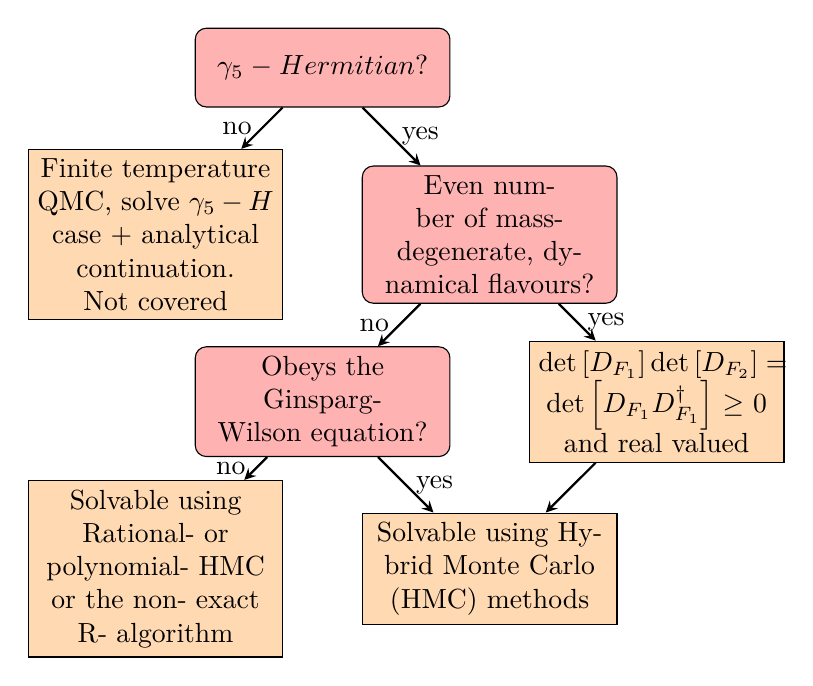
\begin{tikzpicture}[node distance=3cm]
\node (q0) [question]{$\gamma_5-Hermitian?$};

\node (a1) [answer,below left of =q0]{Finite temperature QMC, solve $\gamma_5-H$ case + analytical continuation. Not covered};
\node (q1) [question,below right of =q0]{Even number of mass- degenerate, dynamical flavours?};

\node (a2) [answer,below right of =q1]{$\operatorname{det}\left[ D_{F_1} \right]\operatorname{det}\left[ D_{F_2} \right]=\operatorname{det}\left[ D_{F_1} D^\dagger_{F_1} \right] \geq 0$ and real valued};
\node (q2) [question,below left of =q1]{Obeys the Ginsparg-Wilson equation?};

\node (a3) [answer,below left of =a2]{Solvable using Hybrid Monte Carlo (HMC) methods};
\node (a4) [answer,below left of =q2]{Solvable using Rational- or polynomial- HMC or the non- exact R- algorithm };


\draw [arrow] (q0) -- node[anchor=west] {yes} (q1);
\draw [arrow] (q0) -- node[anchor=east] {no} (a1);

\draw [arrow] (q1) -- node[anchor=west] {yes} (a2);
\draw [arrow] (q1) -- node[anchor=east] {no} (q2);

\draw [arrow] (q2) -- node[anchor=west] {yes} (a3);
\draw [arrow] (q2) -- node[anchor=east] {no} (a4);

\draw [arrow] (a2) -- (a3);
\end{tikzpicture}
\caption[Dynamical fermions- decision chart for update algorithms]{Decision chart for update algorithms based on the properties of the Dirac-operator being simulated. The options are by no means extensive and only reflect the most popular choices in modern LQCD simulations \cite{schaefer2012status}.}
\end{figure}

\paragraph{Pseudofermions and Monte Carlo methods}
We will not cover HMC with Ginsparg-Wilson fermions of arbitrary flavour number, which are covered in \cite{DeGrand:2006ws} using the overlap operator. We instead focus on the case for two degenerate, light quark flavours.\\\\ The expectation value for an observable can be rewritten as
\begin{equation}\label{eq:exp_val_w_pf}
\begin{aligned} 
\braket{O}&=\frac{1}{Z} \int \mathcal{D}[U] \mathrm{e}^{-S_{G}[U]} \operatorname{det}\left[D_{u}\right] \operatorname{det}\left[D_{d}\right] \braket{O}_{F}\\&=\frac{1}{Z} \int \mathcal{D}[U] \mathrm{e}^{-S_{G}[U]} \operatorname{det}\left[DD^\dagger\right]\braket{O}_{F}\\&=\frac{\pi^{-N_F}}{Z} \int \mathcal{D}[U]\mathcal{D}\left[\phi_{R}\right] \mathcal{D}\left[\phi_{I}\right] \mathrm{e}^{-S_{G}[U]-\phi^{\dagger}\left(D D^{\dagger}\right)^{-1} \phi}  \braket{O}_{F}
\end{aligned}
\end{equation}
where in the third line, we've used a result from \cite{WeingartenD.H1981MCif}, expressing $\operatorname{det}\left[DD^\dagger\right]$ in terms of the integral over so- called pseudofermion fields. These have bosonic statistics, but an equal number of degrees of freedom to the fermionic fields, i.e. Dirac-,color- and space-time indices. $\pi$ is an irrelevant overall factor.\\\\What \eqref{eq:exp_val_w_pf} tells us is that rather than evaluating the determinant, we can instead sample gauge configurations from a probability measure similar to that of pure gauge theory (see \eqref{eq:prob_measure}). In the pure gauge theory calculation, we sampled gauge configurations using the Metropolis algorithm, where a single link was chosen and a new configuration $U^\prime$ selected according to some symmetric selection probability $T_0\mkern-4mu\left(U^{\prime}\mkern-6mu \mid\mkern-5mu U\right)$, then the change was accepted if
\begin{equation}
T\mkern-4mu\left(U^{\prime}\mkern-6mu \mid\mkern-5mu U\right)_A = \min (1, \exp (S[U]-S\left[U^{\prime}\right]))
\end{equation}
exceeded a uniformly distributed random variable.
We then leveraged the fact that the action was local in the link variables so that we only needed to calculate $S_{local}[U]-S_{local}\left[U^{\prime}\right]$, a much simpler task. But now, with dynamical fermions switched on, we have 
\begin{equation}
\exp \left(S[U]-S\left[U^{\prime}\right]\right)=\exp \left(S_{G}[U]-S_{G}\left[U^{\prime}\right]\right) \exp \left(S_{\mathrm{F}}^{\mathrm{eff}}[U]-S_{\mathrm{F}}^{\mathrm{eff}}\left[U^{\prime}\right]\right)
\end{equation}
with $S_{\mathrm{F}}^{\mathrm{eff}}[U] =\phi^{\dagger}\left(D[U] D^{\dagger}[U]\right)^{-1} \phi $, which is by no means a local action. This means that every time we proposed a change in a link variable, we would have to calculate the entire global effective action. If the entire action is going to change anyway, we might as well update several link variables between accept-reject steps. Doing this in a way that leads to acceptable acceptance- rates and autocorrelation times is the goal of the next section.
\subsection{Hybrid Monte Carlo}\label{HMC}
HMC is an instance of the Metropolis-Hastings algorithm where proposed configurations are generated according to Hamiltonian time evolution using a numerical integrator. This integrator is subject to two conditions, due to the detailed balance condition, which are reversibility and volume preservation. The usual candidate (and the one we will be working with) is the leapfrog integrator. This integrator is subject to a discretization error, which can be corrected by including an accept-reject step akin to that of regular Monte Carlo.\\\\As for a system of classical particles, we define a Hamiltonian and a configuration space consisting of the field values $Q$ and their conjugate momenta $P$. In the case of $SU(3)$, we define $Q$ and $P$ to be elements of the algebra
\begin{equation}
Q_{\mu}(n) = \sum_{i=1}^{8} \omega_{\mu}^{i}(n) T_{i},\quad P_{\mu}(n)=\sum_{i=1}^{8} P_{\mu}^{i}(n) T_{i}
\end{equation}
such that $P_{\mu}^{i}(n)$ are conjugate to $\omega_{\mu}^{i}(n)$ and 
$Q_{\mu}(n)=i\operatorname{ln}U_{\mu}(n).$
The corresponding classical equations of motion for the Hamiltonian
\begin{equation}
H =\operatorname{tr}\left[P^{2}\right]+S_{G}[U]
+\phi^{\dagger}\left(D D^{\dagger}\right)^{-1} \phi
\end{equation}
are
\begin{equation}
\begin{aligned}
\dot{P} &=-\frac{\partial H}{\partial Q}=-\sum_{i=1}^{8} T_{i} \nabla^{i}\left(S_{G}[U]+\phi^{\dagger}\left(D D^{\dagger}\right)^{-1} \phi\right) =  -F[U, \phi]\\
\dot{Q} &=\frac{\partial H}{\partial P}=P.
\end{aligned}
\end{equation}
for 
\begin{equation}\label{eq:group_derivative}
\nabla^{i} f(U) \equiv \frac{\partial f(U)}{\partial \omega^{i}}=\left.\frac{\partial}{\partial \omega} f\left(\mathrm{e}^{\mathrm{i} \omega T_{i}} U\right)\right|_{\omega=0}
\end{equation}
\cite{Gattringer:2010zz}.
The leapfrog integrator for the system of equations is then
\begin{equation}\label{eq:leapfrog_evolution}
\begin{array}{ll}
U_{(0)} & P_{(0)} \\
 & \downarrow\\\Bigg\downarrow &P_{\left(\frac{1}{2}\right)}=P_{(0)}-\frac{\varepsilon}{2}F\left[ U_{(0)},\phi \right]  \\ &\downarrow
\\
U_{(1)}=\exp \left(\mathrm{i} \varepsilon P_{\left(\frac{1}{2}\right)}\right) U_{(0)} & P_{(1)}=P_{\left(\frac{1}{2}\right)}-\frac{\varepsilon}{2}F\left[ U_{(1)},\phi \right].
\end{array}
\end{equation}
Several leapfrog steps can be combined by inserting a set of complete steps (step size $\varepsilon$) for $U$ and $P$ before the last half step. If the integrator was exact, then the equations of motion would transport the link variables along paths in configuration space with constant energy and therefore give an acceptance probability of $1$. \paragraph{Exponentiating algebra elements of non-Abelian groups} can be computationally expensive, truncating an exponential series expansion with an associated error. Therefore, the Cayley-Hamilton theorem is often used to simplify the calculation. It states that any square matrix over a commutative ring is a solution to its own characteristic polynomial. The characteristic polynomial of a $3\times3$ matrix can be expressed as
\begin{equation}
p(\lambda)=\lambda^{3}-\operatorname{tr}(M) \lambda^{2}+\frac{1}{2}\left(\operatorname{tr}(M)^{2}-\operatorname{tr}\left(M^{2}\right)\right) \lambda-\operatorname{det}(M).
\end{equation}
Because $P \in su(3)$, it must be traceless and Hermitian in addition to being in the $ \operatorname{GL}(3,c)$ representation of $su(3)$. This means that the characteristic polynomial equation $P$ can be written as
\begin{equation}\label{eq:char_poly_P}
P^{3}-\frac{1}{2}\operatorname{tr}\left(P^{2}\right)P-\frac{1}{3}\operatorname{tr}(P^3) = 0
\end{equation}
where we have used an identity of $3\times3$ matrices to re-express the determinant of $P$ in terms of the trace of its cube. \eqref{eq:char_poly_P} defines a recursive relationship for all powers $P^n\,\mid\,n\geq3$ by left or right multiplication with $P$, which means that the matrix exponent series expansion 
\begin{equation}
\exp (iP)=\sum_{k=0}^{\infty} \frac{(iP)^{k}}{k !}=I_{3\times3}+iP-\frac{1}{2} P^{2}-\frac{1}{6}i P^{3}+\cdots
\end{equation}
is ultimately a function linear in the matrices $P$ and $P^2$ with coefficients which depend on $\operatorname{tr}(P^2)$ and $\operatorname{tr}(P^3)$ which need only be calculated once. Following the procedure in \cite{morningstar2004analytic}, we attempt to solve 
\begin{equation}\label{eq:Cay_ham_eq}
e^{i P}=f_{0} I+f_{1} P+f_{2} P^{2} 
\end{equation}
for the three coefficients $f_i$. The three eigenvalues of $P$, denoted $p_1,\,p_2,\,p_3$ are parametrized as 
\begin{equation}
\begin{aligned}
&p_{1}=2 u \\
&p_{2}=-u+w\\
&p_{3}=-p_{1}-p_{2}=-u-w
\end{aligned}
\,\,\,\,\,
\begin{aligned}
&u=\sqrt{\frac{1}{6}\operatorname{Tr}\left(Q^{2}\right)} \cos \left(\frac{1}{3} \theta\right) \\
&w=\sqrt{\frac{1}{2} \operatorname{Tr}\left(Q^{2}\right)} \sin \left(\frac{1}{3} \theta\right) \\
&\theta=\arccos \left(\frac{\frac{1}{3} \operatorname{Tr}\left(Q^{3}\right)}{\left(\frac{ \operatorname{Tr}\left(Q^{2}\right)}{3}\right)^{3 / 2}}\right)
\end{aligned}.
\end{equation}
They are subsequently used to diagonalize $P$, which reduces \eqref{eq:Cay_ham_eq} to a system of linear equations
\begin{equation}
\left[\begin{array}{lll}
1 & p_{1} & p_{1}^{2} \\
1 & p_{2} & p_{2}^{2} \\
1 & p_{3} & p_{3}^{2}
\end{array}\right]\left[\begin{array}{l}
f_{0} \\
f_{1} \\
f_{2}
\end{array}\right]=\left[\begin{array}{c}
e^{i p_{1}} \\
e^{i p_{2}} \\
e^{i p_{3}}
\end{array}\right]
\end{equation}
Morningstar and Peardon isolate the numerical instability in a term $\xi_{0}(w)=\frac{\sin w}{w}$ which can be separately evaluated as 
\begin{equation}
\xi_{0}(w)= \begin{cases}1-\frac{1}{6} w^{2}\left(1-\frac{1}{20} w^{2}\left(1-\frac{1}{42} w^{2}\right)\right), & |w| \leqslant 0.05 \\ \sin (w) / w, & |w|>0.05\end{cases}
\end{equation}
and give the coefficients as 
\begin{equation}\label{eq:f_coeffs_equation}
f_{j}=\frac{h_{j}}{\left(9 u^{2}-w^{2}\right)}
\end{equation}
for 
\begin{equation}
\begin{aligned}
h_{0}=&\left(u^{2}-w^{2}\right) e^{2 i u}+e^{-i u}\left\{8 u^{2} \cos (w)\right.\\
&\left.+2 i u\left(3 u^{2}+w^{2}\right) \xi_{0}(w)\right\} \\
h_{1}=& 2 u e^{2 i u}-e^{-i u}\{2 u \cos (w)\\
&\left.-i\left(3 u^{2}-w^{2}\right) \xi_{0}(w)\right\} \\
h_{2}=& e^{2 i u}-e^{-i u}\left\{\cos (w)+3 i u \xi_{0}(w)\right\}
\end{aligned}
\end{equation}
The final numerical instability in the denominator of \eqref{eq:f_coeffs_equation} is removed by identifying cases where $\frac{1}{3} \operatorname{Tr}\left(Q^{3}\right)<0$ and exploiting the symmetry relation 
$$
f_{i}\left(-\frac{1}{3} \operatorname{Tr}\left(Q^{3}\right), \frac{1}{2} \operatorname{Tr}\left(Q^{2}\right)\right)=(-)^{i} f_{i}^{*}\left(\frac{1}{3} \operatorname{Tr}\left(Q^{3}\right), \frac{1}{2} \operatorname{Tr}\left(Q^{2}\right)\right)
$$
to instead evaluate only the positive case, and apply the above relation for the negative case after the evaluation.
\paragraph{HMC algorithm}The most expensive part of the HMC algorithm is the computation of $F[U, \phi]$, which involves differentiating $D$ according to \eqref{eq:group_derivative} and taking the inverse of $DD^\dagger$. Any computationally sound implementation will be unique depending on the properties of the Dirac operator in question. Special attention must be paid when differentiating Dirac operators that are not strictly linear in the gauge fields, as $SU(3)$ is not a commutative group.\\\\In \eqref{eq:leapfrog_evolution}, the pseudofermion field $\phi$ is treated as a constant, external field. So before updating $P$ and $Q$, we first have to update $\phi$ according to the distribution
\begin{equation}
\begin{aligned} 
 \exp&\left(- \phi^{\dagger}\left(D D^{\dagger}\right)^{-1} \phi \right)
\\ = \exp&\left(- \phi^{\dagger} \left( D^{\dagger} \right)^{-1}D^{-1} \phi \right)\\=  \exp&\left(- \left( D\chi \right)^{\dagger} \left( D^{\dagger} \right)^{-1}D^{-1} \left( D\chi \right) \right)\\ = \exp&\left(- \chi^{\dagger} \chi  \right),\,\,\phi = D\chi.
\end{aligned}
\end{equation}
We are now ready to state the algorithm for the full HMC update step which can be found in listing \ref{alg:HMCalg}. Here, $P$ and $Q$ carry suppressed lattice and Dirac- indices i.e. $P^{\mu,n}_{(k)},\,U^{\mu,n}_{(k)}\rightarrow P_{(k)},\,U_{(k)}$ with the exception of the real numbers $P_{\mu}^{i}(n)$ which parametrize the generator expansion of the algebra elements $P_{\mu}(n)$. $P^2$ denotes the sum $\sum\limits_{\mu,n} P_{\mu}(n)^2$.
\begin{algorithm}
\caption{HMC updating algorithm}\label{alg:HMCalg}
\begin{algorithmic}

\Ensure 
\State $\chi \sim \exp\left(- \chi^{\dagger} \chi  \right)$
\State $\phi = D\chi$
\State $\left\{P_{\mu}^{i}(n)\, \mid \, P_{\mu}^{i}(n)\sim \exp \left(-\operatorname{tr}\left[P^{2}\right]\right)\,\forall\,\{\mu,n\}\in \Lambda \right\}$
\State $F\left[ U_{(0)},\phi \right]$
\State $P_{\left(\frac{1}{2}\right)}=P_{(0)}-\frac{\varepsilon}{2}F\left[ U_{(0)},\phi \right]$

\While{$k\leq n-1$}\Comment{Full steps between half-steps, typically $n\approx 1/\varepsilon$}
\State $U_{(k)}=\exp \left(\mathrm{i} \varepsilon P_{\left(k-\frac{1}{2}\right)}\right) U_{(k-1)}$
\State $P_{\left(k+\frac{1}{2}\right)}=P_{\left(k-\frac{1}{2}\right)}-\varepsilon F\left[ U_{(k)},\phi \right]$
\State $ k+=1$
\EndWhile
\State $U_{(n)}=\exp \left(\mathrm{i} \varepsilon P_{\left(n-\frac{1}{2}\right)}\right) U_{(n-1)}$
\State $P_{\left(n\right)}=P_{\left(n-\frac{1}{2}\right)}-\frac{\varepsilon}{2} F\left[ U_{(n)},\phi \right]$\\
\State Calculate $\exp (-\Delta H)$
\State Generate a random, uniformly distributed number $r \in [0,1) $
\If{$\exp (-\Delta H)\geq r$}
    \State $U \gets U_{new}$
\Else
    \State $U \gets U_{old}$
\EndIf

\end{algorithmic}
\end{algorithm}
It can be shown \cite{DUANE1987216} that this algorithm obeys the necessary detailed balance condition. The step size $\varepsilon$ must be controlled so as to make the discretization error small enough for a large acceptance probability. Recall that if the integrator was exact, the Monte- Carlo step would accept every update. 
\subsection{Other algorithms for dynamical fermions}
We would often like to go without the restriction of using an even number of mass degenerate, dynamical quark flavours. In addition, working with Ginsparg- Wilson fermions in HMC can make the evaluation of the force term very costly. Several algorithms have been proposed to deal with these scenarios, either working to make HMC compatible with odd numbers of dynamical quark flavours or by using non- exact methods with mitigating procedures to reduce errors.
\paragraph{The R-algorithm}\cite{PhysRevD.35.2531} calculates the change in the effective fermion action by the linear approximation 
\begin{equation}
\begin{aligned}
\Delta S_{\mathrm{F}}^{\mathrm{eff}} &=S_{\mathrm{F}}^{\mathrm{eff}}\left[U_{\mu}(n)^{\prime}\right]-S_{\mathrm{F}}^{\mathrm{eff}}\left[U_{\mu}(n)\right] \\
&=\sum_{n, \mu, i} \frac{\partial S_{\mathrm{F}}^{\mathrm{eff}}\left[U_{\mu}(n)\right]}{\partial \omega_{\mu}^{(i)}(n)} \Delta \omega_{\mu}^{(i)}(n)+\mathcal{O}\left(\left(\Delta \omega_{\mu}^{(i)}(n)\right)^{2}\right)
\end{aligned}
\end{equation}
and, by assuming that $\operatorname{det}[D]$ is real-valued and strictly positive, the derivative can be expressed as
\begin{equation}
\frac{\partial S_{\mathrm{F}}^{\text {eff }}}{\partial \omega_{\mu}^{(i)}(n)}=-\frac{\partial \operatorname{tr}[\ln (D[U])]}{\partial \omega_{\mu}^{(i)}(n)}=-\operatorname{tr}\left[D[U]^{-1} \frac{\partial D[U]}{\partial \omega_{\mu}^{(i)}(n)}\right].
\end{equation} 
This method has a discretization error which must be dealt with by computing observables for decreasing step sizes, then extrapolating to zero step size.\\This arrangement is clearly not optimal as it requires multiple costly simulations just to remove the discretization error. It's a major reason why most modern simulations use one of the exact modified HMC schemes.
\paragraph{Polynomial HMC}
$\operatorname{det} D$ on its own, can not be implemented in standard HMC as in \eqref{eq:exp_val_w_pf}. Instead, it was noticed that, assuming $\operatorname{det} D$ is positive (this assumption does not seem a reasonable one, we'll cover this shortly), it can be expressed in the following way:
\begin{equation}
D^{-1} \approx P_{n} = \prod_{i=1}^{n}\left(D-z_{i}\right)
\end{equation}
where the roots $z_i$ of $P_{n}$ come in complex conjugate pairs for $n=2m$. Using this, along with the assumption of $\gamma_5$-hermiticity we find
\begin{equation}
P_{2 m}=\prod_{i=1}^{m}\left(D-z_{2 i-1}\right)\left(D-z_{2 i-1}\right)^\dagger = T_mT_m^\dagger.
\end{equation}
Therefore, the determinant of $D$ can be expressed as
\begin{equation}
\operatorname{det}(D)=C_{m} \operatorname{det}\left(T_{m}^{\dagger} T_{m}\right)^{-1}
\end{equation}
with the corrective factor 
\begin{equation}
C_{m}= \operatorname{det}\left(DT_{m}^{\dagger} T_{m}\right)
\end{equation}
going to $1$ in the limit $m\rightarrow \infty$. This gives an effective pseudofermion action
\begin{equation}
S=-\phi^{\dagger} T_{n}^{\dagger}(D) T_{n}(D) \phi
\end{equation}
\cite{BORICI1995645}. The above approximation can also be made using rationals, giving their name of rational HMC.\\On our earlier assumption that $\operatorname{det}D$ is positive, this clearly needs to be justified, as there is no visible constraint making this assumption true. This is known as the "sign problem" in LQCD\footnote{This is but one part of a larger class of problems in numerical physics dealing with partition functions of fermions (especially at non- zero chemical potential, recall that $\gamma_5$-hermiticity ensures the reality of the determinant) broadly known as the numerical sign problem.}, and it can be treated in a couple of ways.\\Firstly, one could just compute the sign of the determinant for every gauge configuration and include it in the average, but this is extremely cost-prohibitive.\\In practice, the assumption is made based on a couple of observations:\\$\operatorname{det}D$ is in fact positive in the continuum limit and this is indicated to hold at the range of lattice spacings and quark masses being used in simulations \cite{BORICI1995645}\cite{Zyla:2020zbs}.\\Secondly, under molecular dynamics evolution as is the case in HMC, the gauge configuration changes continuously and therefore also the eigenvalues of $D$. For an eigenvalue to change sign, it must cross zero, making $\operatorname{det}D$ vanish, and thus suppressing updates along such a trajectory \cite{JLQCD:2001ucs}.\\\\Many other algorithms exist for simulating dynamical fermions. A brief review of some of them can be found in \cite{schaefer2012status}.
\section{Extrapolation}
There are only a few free parameters in a LQCD program. These are the parameters for which we set a number in the program and they are the bare quark masses $m_f$, the inverse gauge coupling $\beta$ and the number of lattice sites which effectively sets the lattice volume through the lattice spacing $a$ which depends on $\beta$ and $m_f$.\par In order to obtain physical results from lattice simulations, one has to extrapolate the results to the continuum- and infinite volume- limit as well as to the physical quark masses if the simulation masses were larger than the physical masses.  
\subsection{The continuum limit}
The fact that we use different lattice actions to simulate seemingly the same physical systems comes from the express understanding that all of these lattice actions share the same universality class\footnote{There has been considerable debate on this point for staggered fermions, see e.g. \cite{BERNARD2007235},\cite{golterman2008qcd},\cite{Creutz2007ReplyT} etc.} i.e. have the same scaling behaviour near critical points, and share the same symmetries relevant to the observable in question. This is important, as taking the continuum limit of a lattice field theory involves driving the couplings to the critical point of the theory corresponding to $a=0$. Therefore, as long as the continuum limit is being considered, different lattice actions will produce the same physical predictions.\par A note of caution before proceeding: Extrapolation to the continuum limit has to be performed at a constant lattice volume. This means that as the couplings are driven towards their critical values, the number of lattice points has to change for every resulting value of $a$ so as to keep the lattice volume from changing.\\\\Keeping $\beta$ constant, the light quark masses $m_u=m_d=m_f$ are tuned to a value $m_f^\star$ where the dimensionless ratios of hadron masses (see \ref{hadron_masses} and \ref{Renormalization}) match the physical predictions. Then the lattice constant is gotten by dividing the hadron mass at the quark mass $m_f^\star$ in lattice units by the physical hadron mass. This procedure is then repeated at several values of $\beta$, allowing us to extrapolate the results to the critical point. Simulations are increasingly being performed at the physical light quark masses, but these may need to be extrapolated based on the available computational resources.
\subsection{The infinite volume limit}
Any simulation will happen at a finite lattice volume, and this impacts the outcomes of observables, as modes that traverse the spatial torus give contributions that would be absent in the infinite volume limit.\\Most simulations are carried out with a temporal extent roughly twice that of the spatial extent to allow excited states to decay. Therefore, the leading contributions are from spatial finite size effects. The largest correlation length in the system arises from the lightest hadron correlator. Volume dependence varies between observables, but for processes involving single particle states, the effects are purported to be sub- leading order for $m_\pi N_sa \geq 4$, where $m_\pi$ is the mass of the pion, the lightest hadron.\\\\The extrapolation can be carried out by increasing the number of spatial lattice points while keeping all other parameters fixed. If possible, the extrapolation might be accompanied by a parametrization based on theory or otherwise a naive power law dependence of the form $\frac{1}{(aN_s)^n}$.

\chapter{Implementation}
At this point, the thesis will change course dramatically. Rather than broadly discussing the theory and practices of quantum field theory and lattice QCD, we move on to tackling the relevant set of issues for answering the problem statement we made at the very beginning of the thesis. These are issues pertaining to the topological charge and the Wilson flow applied to ensembles of pure gauge configurations. We will also tackle the workings of LGF and the particular details associated with implementing lattice QCD simulations in the real world.\\\\As stated numerous times, measuring observables in lattice QCD is effectively partitioned into two separate problems: generating gauge configurations and analysing those configurations. For us, this analysis includes the application of the Wilson flow, accompanied by measurements of observables at several flow steps. We tackle the problem of generation first.
\section{Generating Gauge Configurations}
There are several considerations at play when deciding the set of ensembles which are worth including in your analysis. There are specific requirements to our particular analysis which influences the choice of ensembles and choice of update algorithm.
\begin{enumerate}
\item Autocorrelation time of the topological charge
\item Negating finite-volume effects
\item Limiting discretization effects, autocorrelation and the numerical cost of the Wilson flow through our choice of $\beta$
\item The need for large statistics
\item The need for continuum extrapolation
\item Estimating the autocorrelation time
\end{enumerate}
We cover these in turn.\\\\The topological charge and its cumulants are infamous for suffering from critical slowing down to a greater extent than other observables. This is known to be a particularly substantial problem for HMC algorithms for which e.g. the effective dynamical critical exponent of the squared topological charge was found to be $5$ in pure gauge theory \cite{2011}. This is often referred to as the topology-freezing problem. This is thought to arise from periodic boundary conditions which, close to the continuum, constrain configurations from changing their topological charge through any continuous deformation\footnote{Think, unwinding a closed loop going through the hole of a doughnut without cutting it}. It has been proposed that using open (Neumann) boundary conditions in the time direction can bypass this issue in \cite{L_scher_2011}. An analysis of this was carried out in \cite{PhysRevD.90.074502}.\\Since we're not analysing dynamical fermions, we're free to choose other update algorithms which do not move along molecular-dynamics trajectories and are more likely to 'tunnel' between topological sectors in configuration space. For example, the overrelaxation algorithm is blatantly not a continuous transformation in configuration space.\\The combination of Heatbath and overrelaxation (HB-OR) has been used in several pure gauge theory analyses of the topological charge \cite{non_gaussianities2015} \cite{PhysRevD.92.094518} with great success which makes it a good choice for our purposes.\\That said, LGF has an implementation of a local variant of HMC based on \cite{Kennedy_1994} which is quite fast compared to the HB-OR algorithm and without a careful analysis of the autocorrelation times for different lattice spacings, I cannot say with confidence whether this algorithm could be a viable option for some range of lattice constants. Some limited analysis has been done on the autocorrelation time of observables in \cite{LHMC_autocorr}, but none for the topological charge.\\\\For finite volume effects, we can consider the fact that the lightest glueball has an energy of about 1.5 GeV. For the topological susceptibility, this is expected to produce very small finite-volume effects for simulation lengths greater than $1fm$ \cite{Del_Debbio_2005}. However, we will mostly rely on an analysis carried out in \cite{non_gaussianities2015}. They use a different definition for the field strength tensor (more on this later) and larger lattice constants than this analysis but there is little reason to doubt its transferability to our situation.\\They found that for $L\geq 1.4fm$, finite size effects on the topological susceptibility were smaller than  $0.5\%$. This was a very high statistics study, so these effect sizes are likely smaller than what we need to consider, however we'll air on the side of caution here.\\\\We would like to simulate with very small lattice constants as this makes the continuum extrapolation less questionable. We would also like very high statistics. These two goals are unfortunately at odds. Lower lattice constants increase autocorrelation time as well as the generation time and the computational cost of the Wilson flow for the same simulation volume by increasing the number of lattice points and the number of flow steps needed.\\This effect on computational effort is substantial to the point where analysing 2000 statistically independent configurations at $\beta=6.0$ is practically trivial compared to analysing 100 such configurations at $\beta=6.46$. Trying to strike a balance here is difficult without a prior analysis of the integrated autocorrelation time.\\\\Because the analysis requires continuum extrapolation and because the smallest lattice spacing requires the most computational effort, it's worthwhile to base your choices for $\beta$ and $|\Lambda|$ on the smallest lattice constant.\\\\Estimating the integrated autocorrelation time is very costly. Rather than incurring that cost for the ensembles used in the analysis, it's preferable to do the analysis on ensembles with a smaller lattice volume, making the assumption that those results will be approximately applicable for the larger lattice volume. 

\section{Simulation parameters}
Keeping all of these factors in mind, we can begin to settle on our choices of simulation parameters.
To determine the lattice spacing $a$ from the inverse coupling $\beta$ we use an interpolation from \cite{Guagnelli_1998}, which is valid for $5.7 \leq \beta \leq 6.57$:
\begin{equation}\label{eq:avBeta_interpolated}
\ln \left(a / r_{0}\right)=-1.6805-1.7139(\beta-6)+0.8155(\beta-6)^{2}-0.6667(\beta-6)^{3}.
\end{equation}
According to the authors, this interpolation is accompanied by a relative error, which increases linearly from $0.3\%$ at $\beta = 5.7$ to $0.6\%$ at $\beta = 6.57$. This relative error has been incorporated by the parametrization 
\begin{equation}
Error_{a/r_0} = \frac{a}{r_0}(0.0034482758621\beta - 0.0166551724138)
\end{equation}
We want to sample the configuration space at roughly evenly spaced values of the lattice spacing, keeping the simulation volume constant. This is to optimize the influence of each ensemble on the final continuum limit, closely grouped values would do a worse job at constraining the extrapolation.\\This is a good point to mention an additional constraint which won't be explained until section \ref{sec:parallelization}: we need the lattice to have an even number of points in each dimension.\\These, along with the constraint that our simulation volume must be larger than $1.4fm$ resulted in the choices shown in figure \ref{fig:choosingBetasAndLambdas}.
\begin{figure}
\centering
\includegraphics{FINALPLOTS/N_v_beta.pdf}
\caption[Choice of $\beta$ and lattice volume]{Choices for $\beta$ and $N$. $L=1.5fm$ produces values which nicely line up with the curve $L/a(\beta)$ at even values of $N$. $a(\beta)$ is as defined in \eqref{eq:avBeta_interpolated}}\label{fig:choosingBetasAndLambdas}
\end{figure}
\paragraph{Thermalization}
For thermalization one has a choice of whether to start with all links set to the trivial link (known as a cold start), or whether to start with every link set to a random element of SU(3) (known as a hot start). Performing both, then seeing when the two initial conditions produce the same outcome on the Monte Carlo chain is one way of estimating the required thermalization. Because the topological charge requires the Wilson flow before it can be analyzed, this would be far too costly. Instead, the number of thermalization steps is chosen to be higher than the estimated integrated autocorrelation time.\\\\Choosing cold starts for our analysis would essentially amount to preferentially sample configurations with a topological charge of zero. This is obviously not an option, so every ensemble uses hot starts.
\paragraph{$N_{OR}/N_{HB}$}
In the combined HB-OR method, an obvious hyper-parameter one could tweak to improve decorrelation would be the number of OR steps used per HB step. This optimization is lattice constant- dependent and would also be specific to the topological charge. Rather than performing an expensive analysis of this relationship with potentially dubious improvement, we choose a ratio of $\frac{N_{OR}}{N_{HB}}=4 $ which has already been used successfully in \cite{PhysRevD.92.094518}.\\\\Finally, we're ready to state our chosen simulation parameters. Using the estimates for the integrated autocorrelation time obtained in section \ref{sec:autoCorr_analysis} we settle at the values in table \ref{tab:SimulationParameters}
\begin{table}
\centering
\caption[Simulation parameters]{Simulation parameters for every generated ensemble. Ensembles with a smaller simulation volume were used to estimate $\tau_int$ for each observable, the values of which can be found in table \ref{tab:IntAutocorrs}. Based on those estimates, the number of decorrelation steps $N_{decorr}^Q$ and $N_{decorr}^E$ were decided. The total number of gauge configurations analysed in observables derivative of $E$ and $Q$ is $N_{meas}^E$ and $N_{meas}^Q$ respectively.}
\label{tab:SimulationParameters}
\begin{tabular}{lcccccccc}
\hline \hline Lattice & $\beta$ & $a[fm]$ & $L[fm]$ &$N_{therm}$ & $N_{decorr}^E$ & $N_{decorr}^Q$& $N_{meas}^E$& $N_{meas}^Q$\\
\hline		   $16^4$ &   $6.0$ & $0.093$ & $1.49$  		 		 &$2000$  	  & $200$		   & $200$		   & $1704$		 & $1704$ \\	  
	  		   $12^4$ & 		&     	  & $1.12$  		 		 &$2000$ 	  & $1$		   	   & $1$  		   & $2000$		 & $2000$\\ \hline 
	  		   $20^4$ &   $6.13$& $0.075$ & $1.51$  		 		 &$2000$ 	  & $200$		   & $200$		   & $1324$		 & $1324$ \\
	  		   $14^4$ & 		&  	 	  & $1.06$  		 		 &$2000$ 	  & $1$		       & $1$  		   & $2000$		 & $2000$\\ \hline
	  		   $24^4$ &   $6.26$& $0.062$ & $1.50$  		 		 &$2000$ 	  & $400$		   & $800$		   & $1204$		 & $614$ \\
	  		   $16^4$ & 		&  	 	  & $1.00$  		 		 &$2000$ 	  & $1$		       & $1$  		   & $2\cdot2000$		 & $2\cdot2000$\\ \hline
	  		   $32^4$ &   $6.46$& $0.047$ & $1.51$  		 		 &$4700$ 	  & $1350$		   & $4050$		   & $645$		 & $215$ \\
	  		   $22^4$ & 		&  	 	  & $1.04$  		 		 &$2000$ 	  & $1$		       & $1$  		   & $2\cdot3000$		 & $2\cdot3000$
\end{tabular}
\end{table}




\section{Observables}
Every definition that follows from here, can be read as being defined from the gauge fields at flow times $t>0$. The extra notation has simply been omitted to make the equations easier to read. The distinction is important, as crucially, the gradient flow produces fields which are free from ultraviolet divergences, making the operators renormalized at all non-vanishing flow times. 
\subsection{Improved Lattice Field-Strength tensor}\label{sec:improvedLatticeFieldStrengthTensor}
For the lattice definition of the field- strength tensor, we look at the $\mathcal{O}\left(a^{4}\right)$ improved implementation demonstrated in \cite{BILSONTHOMPSON20031}. A general $m\times n$ Wilson loop operator is defined by the path- ordered exponential of the closed loop integral around the loop:
\begin{equation}
W_{\mu \nu}^{(m \times n)}=\mathscr{P} \mathrm{e}^{\mathrm{ig} \oint A \mathrm{~d} x}
\end{equation}
with 
\begin{equation}\label{eq:WilsonLoopExpansionLoopIntegral}
\begin{aligned}
\oint A \mathrm{~d} x=& \int_{-m a / 2}^{m a / 2} \mathrm{~d} x_{\mu} \int_{-n a / 2}^{n a / 2} \mathrm{~d} x_{v}\left(F_{\mu v}\left(x_{0}\right)+\left\{x_{\mu} \partial_{\mu}+x_{v} \partial_{v}\right\} F_{\mu v}\left(x_{0}\right)\right.\\
&+\left\{x_{\mu} x_{v} \partial_{\mu} \partial_{v}\right\} F_{\mu v}\left(x_{0}\right)+\frac{1}{2}\left\{x_{\mu}^{2} \partial_{\mu}^{2}+x_{v}^{2} \partial_{v}^{2}+x_{\mu}^{2} x_{v} \partial_{\mu}^{2} \partial_{v}\right.\\
&\left.+x_{\mu} x_{v}^{2} \partial_{\mu} \partial_{v}^{2}\right\} F_{\mu v}\left(x_{0}\right)+\frac{1}{6}\left\{x_{\mu}^{3} \partial_{\mu}^{3}+x_{v}^{3} \partial_{v}^{3}+x_{\mu}^{3} x_{v} \partial_{\mu}^{3} \partial_{v}\right.\\
&\left.+x_{\mu} x_{v}^{3} \partial_{\mu} \partial_{v}^{3}\right\} F_{\mu v}\left(x_{0}\right)+\frac{1}{24}\left\{x_{\mu}^{4} \partial_{\mu}^{4}+x_{v}^{4} \partial_{v}^{4}\right\} F_{\mu v}\left(x_{0}\right) \\
&\left.+\frac{1}{4}\left\{x_{\mu}^{2} x_{v}^{2} \partial_{\mu}^{2} \partial_{v}^{2}+x_{\mu}^{2} x_{v}^{2} \partial_{\mu}^{2} \partial_{v}^{2}\right\} F_{\mu v}\left(x_{0}\right)+\mathcal{O}\left(x^{5}\right)\right) 
\end{aligned}
\end{equation}
\cite{BILSONTHOMPSON20031}. This exponential can be expanded in the usual way to get 
\begin{equation}
\mathscr{P} \mathrm{e}^{\mathrm{i} g \oint A \mathrm{~d} x}=\mathscr{P}\left\{1+\mathrm{i} g \oint A \mathrm{~d} x-\frac{g^{2}}{2}(\oint A \mathrm{~d} x)^{2}+\cdots\right\}.
\end{equation}
To arrive at the term proportional to the field strength tensor in $\mathrm{i} g \oint A \mathrm{~d} x$ we observe that by subtracting the hermitian conjugate, every other term is removed and by subtracting a third of the trace, the traceless property is ensured. We get
\begin{equation}\label{eq:cloverToFST}
-\frac{i}{2}\left( W_{\mu \nu}^{(m \times n)}- W_{\mu \nu}^{(m \times n)\dagger} - \frac{1}{3}\operatorname{Tr}\left( W_{\mu \nu}^{(m \times n)}- W_{\mu \nu}^{(m \times n)\dagger} \right)  \right) = g \mathscr{P} \oint A \mathrm{~d} x+\mathcal{O}\left(g^{3}\right)
\end{equation}
\\\\The authors' improved field strength tensor takes the form 
\begin{equation}\label{eq:Improved_lattice_field_strength_tensor}
F_{\mu v}^{\operatorname{Imp}}=k_{1} C_{\mu v}^{(1,1)}+k_{2} C_{\mu v}^{(2,2)}+k_{3} C_{\mu v}^{(1,2)}+k_{4} C_{\mu v}^{(1,3)}+k_{5} C_{\mu v}^{(3,3)}
\end{equation}
wherein 
\begin{equation}
\begin{aligned}
&C^{(1,1)}=\mathscr{A}+\frac{1}{6} \mathscr{B}+\frac{1}{120} \mathscr{C}+\frac{1}{36} \mathscr{D} \\
&C^{(2,2)}=4 \mathscr{A}+\frac{8}{3} \mathscr{B}+\frac{8}{15} \mathscr{C}+\frac{16}{9} \mathscr{D} \\
&C^{(1,2)}=2 \mathscr{A}+\frac{5}{6} \mathscr{B}+\frac{17}{120} \mathscr{C}+\frac{2}{9} \mathscr{D} \\
&C^{(1,3)}=3 \mathscr{A}+\frac{5}{2} \mathscr{B}+\frac{41}{40} \mathscr{C}+\frac{3}{4} \mathscr{D} \\
&C^{(3,3)}=9 \mathscr{A}+\frac{27}{2} \mathscr{B}+\frac{243}{40} \mathscr{C}+\frac{81}{4} \mathscr{D}
\end{aligned}
\end{equation}
for 
\begin{equation}
\begin{aligned}
&\mathscr{A}=g a^{2} F_{\mu \nu} \\
&\mathscr{B}=g a^{4}\left(\partial_{\mu}^{2}+\partial_{v}^{2}\right) F_{\mu \nu} \\
&\mathscr{C}=g a^{6}\left(\partial_{\mu}^{4}+\partial_{v}^{4}\right) F_{\mu v} \\
&\mathscr{D}=g a^{6}\left(\partial_{\mu}^{2} \partial_{v}^{2}\right) F_{\mu v}.
\end{aligned}
\end{equation}
give terms we recognize from equation \eqref{eq:WilsonLoopExpansionLoopIntegral}.
The coefficients $k_i$ must then be tuned to eliminate all contributions from terms $\mathscr{B},\,\mathscr{C}\,and\,\mathscr{D}$. This amounts to solving the linear system of equations 
\begin{equation}
\left[\begin{array}{ccccc}
1 & 4 & 2 & 3 & 9 \\
\frac{1}{6} & \frac{8}{3} & \frac{5}{6} & \frac{5}{2} & \frac{27}{2} \\
\frac{1}{120} & \frac{8}{15} & \frac{17}{120} & \frac{41}{40} & \frac{243}{40} \\
\frac{1}{36} & \frac{16}{9} & \frac{2}{9} & \frac{3}{4} & \frac{81}{4}
\end{array}\right]\left[\begin{array}{l}
k_{1} \\
k_{2} \\
k_{3} \\
k_{4} \\
k_{5}
\end{array}\right]=\left[\begin{array}{c}
1 \\
0 \\
0 \\
0
\end{array}\right] \rightarrow \left[\begin{array}{l}
k_{1} \\
k_{2} \\
k_{3} \\
k_{4} \\
k_{5}
\end{array}\right] = \left[\begin{array}{l}
\frac{19}{9}-55 k_{5} \\
\frac{1}{36}-16 k_{5} \\
64 k_{5}-\frac{32}{45} \\
\frac{1}{15}-6 k_{5} \\
k_{5}
\end{array}\right].
\end{equation}
Here $k_{5}$ is a free parameter, and it allows us to eliminate one of the terms in \eqref{eq:IlfstFin}. A good choice is $k_{5} = 0$, which allows us to ignore the $C_{\mu v}^{(3,3)}$ term. The improved lattice field strength tensor now looks like  

\begin{equation}\label{eq:IlfstFin}
F_{\mu v}^{\operatorname{Imp}}=\frac{19}{9} C_{\mu v}^{(1,1)}+\frac{1}{36} C_{\mu v}^{(2,2)}+\frac{32}{45} C_{\mu v}^{(1,2)}+\frac{1}{15} C_{\mu v}^{(1,3)}.
\end{equation}
The terms $C^{(m,n)}$ are so called clover terms which can be calculated on the lattice by evaluating the set of $m\times n$ Wilson loops which immediately surround the lattice site. Those terms which are found in \eqref{eq:IlfstFin} are illustrated in figure \ref{fig:Clovers}.
\begin{figure}
\centering
\begin{subfigure}[b]{0.4\textwidth}
\centering
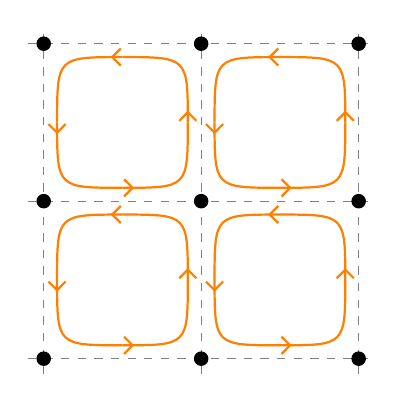
\begin{tikzpicture}

    \foreach \x in {0,1,2}
    {
        \foreach \y in {0,1,2}
        {
            \coordinate (n\x\y) at ($\x*(20mm, 0)+\y*(0, 20mm)$);
        }
    }

    \draw[style=help lines,dashed] (-0.2, 0) -- (4.2, 0);
    \draw[style=help lines,dashed] (-0.2, 2) -- (4.2, 2);
    \draw[style=help lines,dashed] (-0.2, 4) -- (4.2, 4);

    \draw[style=help lines,dashed] (0, -0.2) -- (0, 4.2);
    \draw[style=help lines,dashed] (2, -0.2) -- (2, 4.2);
    \draw[style=help lines,dashed] (4, -0.2) -- (4, 4.2);

    \newcommand\cloverlink{
        \draw[link arrow, thick] (3, 2.17) .. controls (3.83, 2.17) and (3.83, 2.17) .. (3.83, 3);
    }

    \newcommand\linkmargin{1.7mm}
    \newcommand\cloverplaquette{
        \cloverlink

        \begin{scope}[transform canvas={rotate around={90:(3, 3)}}]
            \cloverlink
        \end{scope}
        \begin{scope}[transform canvas={rotate around={180:(3, 3)}}]
            \cloverlink
        \end{scope}
        \begin{scope}[transform canvas={rotate around={270:(3, 3)}}]
            \cloverlink
        \end{scope}
    }

    \cloverplaquette
    \begin{scope}[transform canvas={rotate around={90:(n11)}}]
        \cloverplaquette
    \end{scope}
    \begin{scope}[transform canvas={rotate around={180:(n11)}}]
        \cloverplaquette
    \end{scope}
    \begin{scope}[transform canvas={rotate around={270:(n11)}}]
        \cloverplaquette
    \end{scope}

    \foreach \x in {0,1,2}
    {
        \foreach \y in {0,1,2}
        {
            \node[lattice point] at (n\x\y) {};
        }
    }



\end{tikzpicture}
\end{subfigure}
%
\begin{subfigure}[b]{0.4\textwidth}
\centering
\scalebox{0.5}{
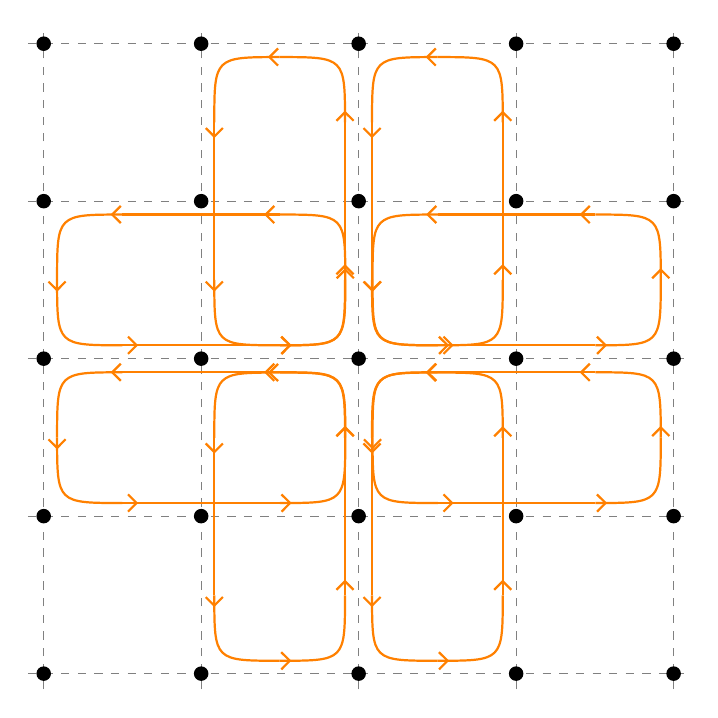
\begin{tikzpicture}

    \foreach \x in {-1,0,1,2,3}
    {
        \foreach \y in {-1,0,1,2,3}
        {
            \coordinate (n\x\y) at ($\x*(20mm, 0)+\y*(0, 20mm)$);
        }
    }
	\newcommand\XMin{-2.2}
	\newcommand\XMax{6.2}
	\draw[style=help lines,dashed] (\XMin, -2) -- (\XMax, -2);
    \draw[style=help lines,dashed] (\XMin, 0) -- (\XMax, 0);
    \draw[style=help lines,dashed] (\XMin, 2) -- (\XMax, 2);
    \draw[style=help lines,dashed] (\XMin, 4) -- (\XMax, 4);
    \draw[style=help lines,dashed] (\XMin, 6) -- (\XMax, 6);
	
	\draw[style=help lines,dashed] (-2, \XMin) -- (-2, \XMax);
    \draw[style=help lines,dashed] (0, \XMin) -- (0, \XMax);
    \draw[style=help lines,dashed] (2, \XMin) -- (2, \XMax);
    \draw[style=help lines,dashed] (4, \XMin) -- (4, \XMax);
    \draw[style=help lines,dashed] (6, \XMin) -- (6, \XMax);

    \newcommand\cloverlink{
        \draw[link arrow, thick] (3, 2.17) .. controls (3.83, 2.17) and (3.83, 2.17) .. (3.83, 3);
        \draw[link arrow, thick] (3.83, 3) -- (3.83, 5);
        \draw[link arrow, thick] (3.83, 5) .. controls (3.83, 5.83) and (3.83, 5.83) .. (3, 5.83);
    }

    \newcommand\linkmargin{1.7mm}
    \newcommand\cloverplaquette{
        \cloverlink

%        \begin{scope}[transform canvas={rotate around={90:(3, 3)}}]
%            \cloverlink
%        \end{scope}
        \begin{scope}[transform canvas={rotate around={180:(3, 4)}}]
            \cloverlink
        \end{scope}
%        \begin{scope}[transform canvas={rotate around={270:(3, 3)}}]
%            \cloverlink
%       \end{scope}

    }
    
    \newcommand\clover{
    \cloverplaquette
    \begin{scope}[transform canvas={xshift=-57pt}]
        \cloverplaquette
    \end{scope}
    \begin{scope}[transform canvas={xshift=-57pt,yshift = -114pt}]
        \cloverplaquette
    \end{scope}
        \begin{scope}[transform canvas={yshift = -114pt}]
        \cloverplaquette
    \end{scope}

    }
    \clover
    \begin{scope}[transform canvas={rotate around={90:(2, 2)}}]
    	\clover
    \end{scope}

    \foreach \x in {-1,0,1,2,3}
    {
        \foreach \y in {-1,0,1,2,3}
        {
            \node[lattice point] at (n\x\y) {};
        }
    }

\end{tikzpicture}
}
\end{subfigure}

\bigskip
\begin{subfigure}[b]{0.4\textwidth}
\centering
\scalebox{0.5}{
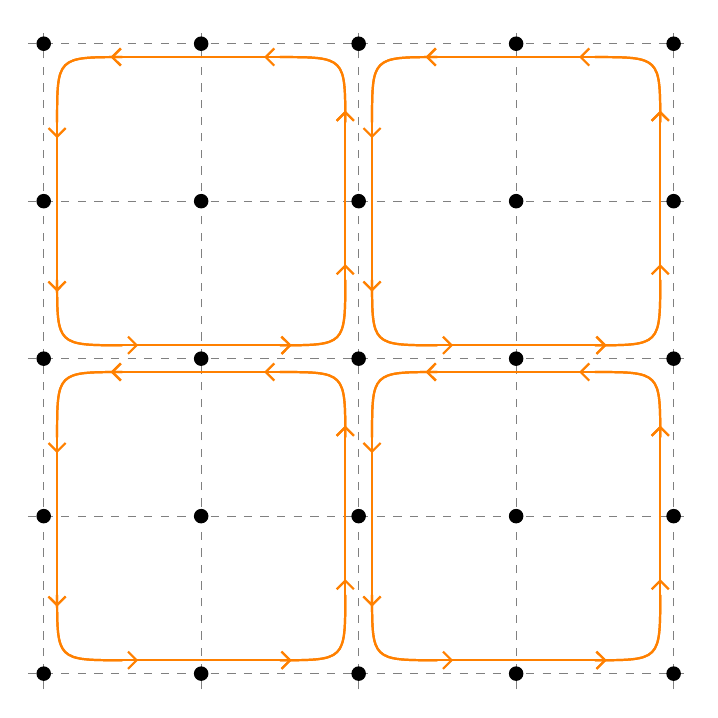
\begin{tikzpicture}

    \foreach \x in {-1,0,1,2,3}
    {
        \foreach \y in {-1,0,1,2,3}
        {
            \coordinate (n\x\y) at ($\x*(20mm, 0)+\y*(0, 20mm)$);
        }
    }
	\newcommand\XMin{-2.2}
	\newcommand\XMax{6.2}
	\draw[style=help lines,dashed] (\XMin, -2) -- (\XMax, -2);
    \draw[style=help lines,dashed] (\XMin, 0) -- (\XMax, 0);
    \draw[style=help lines,dashed] (\XMin, 2) -- (\XMax, 2);
    \draw[style=help lines,dashed] (\XMin, 4) -- (\XMax, 4);
    \draw[style=help lines,dashed] (\XMin, 6) -- (\XMax, 6);
	
	\draw[style=help lines,dashed] (-2, \XMin) -- (-2, \XMax);
    \draw[style=help lines,dashed] (0, \XMin) -- (0, \XMax);
    \draw[style=help lines,dashed] (2, \XMin) -- (2, \XMax);
    \draw[style=help lines,dashed] (4, \XMin) -- (4, \XMax);
    \draw[style=help lines,dashed] (6, \XMin) -- (6, \XMax);

    \newcommand\cloverlink{
        \draw[link arrow, thick] (5, 2.17) .. controls (5.83, 2.17) and (5.83, 2.17) .. (5.83, 3);
        \draw[link arrow, thick] (5.83, 3) -- (5.83, 5);
        \draw[link arrow, thick] (5.83, 5) .. controls (5.83, 5.83) and (5.83, 5.83) .. (5, 5.83);
    }

    \newcommand\linkmargin{1.7mm}
    \newcommand\cloverplaquette{
        \cloverlink

        \begin{scope}[transform canvas={rotate around={90:(4, 4)}}]
            \cloverlink
        \end{scope}
        \begin{scope}[transform canvas={rotate around={180:(4, 4)}}]
            \cloverlink
        \end{scope}
        \begin{scope}[transform canvas={rotate around={270:(4, 4)}}]
            \cloverlink
       \end{scope}

    }

    \cloverplaquette
    \begin{scope}[transform canvas={rotate around={90:(n11)}}]
        \cloverplaquette
    \end{scope}
    \begin{scope}[transform canvas={rotate around={180:(n11)}}]
        \cloverplaquette
    \end{scope}
    \begin{scope}[transform canvas={rotate around={270:(n11)}}]
        \cloverplaquette
    \end{scope}

    \foreach \x in {-1,0,1,2,3}
    {
        \foreach \y in {-1,0,1,2,3}
        {
            \node[lattice point] at (n\x\y) {};
        }
    }

\end{tikzpicture}
}
\end{subfigure}
%
\begin{subfigure}[b]{0.4\textwidth}

\centering
\scalebox{0.333}{
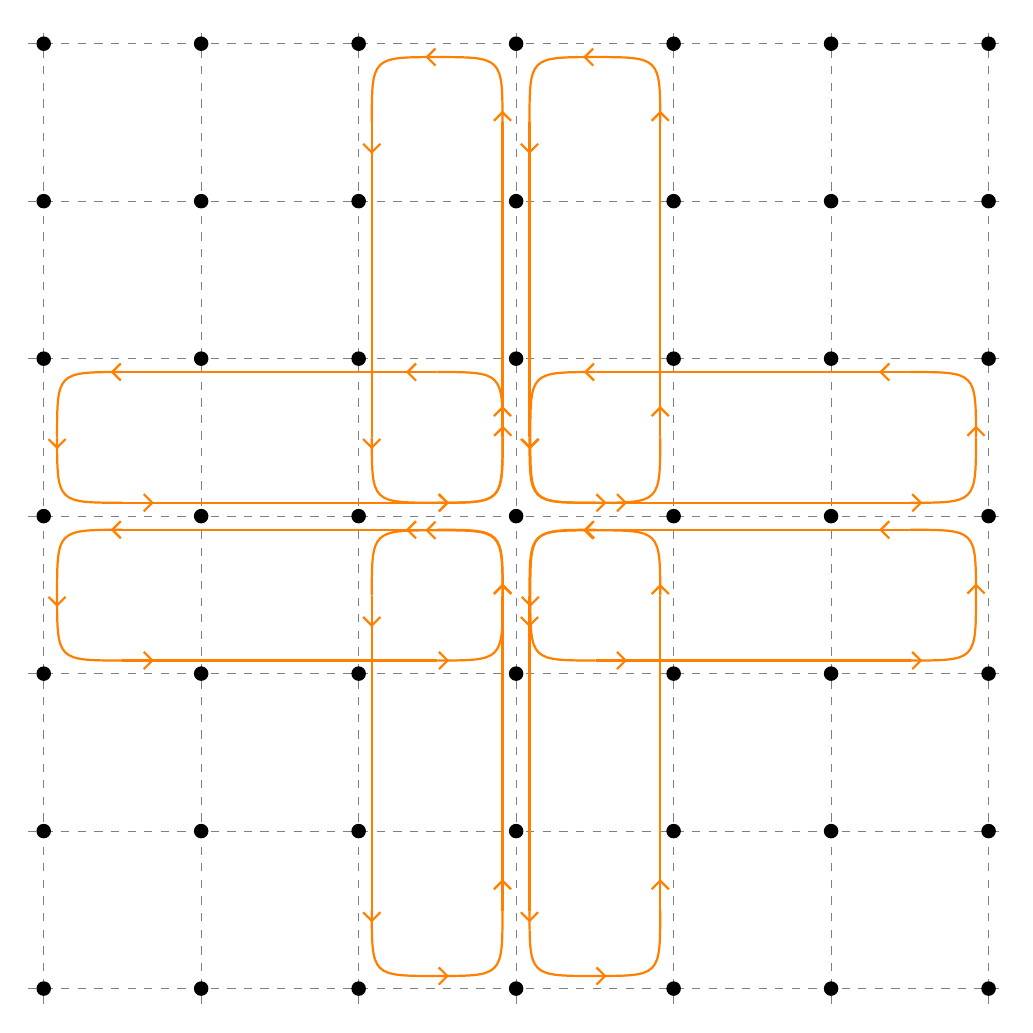
\begin{tikzpicture}

    \foreach \x in {-2,-1,0,1,2,3,4}
    {
        \foreach \y in {-2,-1,0,1,2,3,4}
        {
            \coordinate (n\x\y) at ($\x*(20mm, 0)+\y*(0, 20mm)$);
        }
    }
	\newcommand\XMin{-4.2}
	\newcommand\XMax{8.2}
	\draw[style=help lines,dashed] (\XMin, -4) -- (\XMax, -4);
	\draw[style=help lines,dashed] (\XMin, -2) -- (\XMax, -2);
    \draw[style=help lines,dashed] (\XMin, 0) -- (\XMax, 0);
    \draw[style=help lines,dashed] (\XMin, 2) -- (\XMax, 2);
    \draw[style=help lines,dashed] (\XMin, 4) -- (\XMax, 4);
    \draw[style=help lines,dashed] (\XMin, 6) -- (\XMax, 6);
	\draw[style=help lines,dashed] (\XMin, 8) -- (\XMax, 8);
	
	\draw[style=help lines,dashed] (-4, \XMin) -- (-4, \XMax);
	\draw[style=help lines,dashed] (-2, \XMin) -- (-2, \XMax);
    \draw[style=help lines,dashed] (0, \XMin) -- (0, \XMax);
    \draw[style=help lines,dashed] (2, \XMin) -- (2, \XMax);
    \draw[style=help lines,dashed] (4, \XMin) -- (4, \XMax);
    \draw[style=help lines,dashed] (6, \XMin) -- (6, \XMax);
    \draw[style=help lines,dashed] (8, \XMin) -- (8, \XMax);

    \newcommand\cloverlink{
        \draw[link arrow, thick] (3, 2.17) .. controls (3.83, 2.17) and (3.83, 2.17) .. (3.83, 3);
        \draw[link arrow, thick] (3.83, 3) -- (3.83, 7);
        \draw[link arrow, thick] (3.83, 7) .. controls (3.83, 7.83) and (3.83, 7.83) .. (3, 7.83);
    }

    \newcommand\linkmargin{1.7mm}
    \newcommand\cloverplaquette{
        \cloverlink
        \begin{scope}[transform canvas={rotate around={180:(3, 5)}}]
            \cloverlink
        \end{scope}
    }
    
    \newcommand\clover{
    \cloverplaquette
    \begin{scope}[transform canvas={xshift=-57pt}]
        \cloverplaquette
    \end{scope}
    \begin{scope}[transform canvas={xshift=-57pt,yshift = -171pt}]
        \cloverplaquette
    \end{scope}
        \begin{scope}[transform canvas={yshift = -171pt}]
        \cloverplaquette
    \end{scope}

    }
    \clover
    \begin{scope}[transform canvas={rotate around={90:(2, 2)}}]
    	\clover
    \end{scope}

    \foreach \x in {-2,-1,0,1,2,3,4}
    {
        \foreach \y in {-2,-1,0,1,2,3,4}
        {
            \node[lattice point] at (n\x\y) {};
        }
    }

\end{tikzpicture}
}
\end{subfigure}
\caption[Lattice field strength tensor clovers]{$C^{(1,1)}$ and $C^{(2,2)}$ contain a factor of $\frac{1}{4}$ since the two terms are symmetric under $n\leftrightarrow m$. $C^{(1,2)}$ and $C^{(1,3)}$ each need to be evaluated for two different orientations and their results added and multiplied by a factor of $\frac{1}{8}$. Thanks to Martin Ueding for providing Tikz templates on \href{https://github.com/HISKP-LQCD/lqcd-tikz-graphics}{\textbf{their github}}.}
\label{fig:Clovers}
\end{figure}
equation \eqref{eq:cloverToFST} can then be applied to each clover term to get the improved field strength tensor from equation \eqref{eq:IlfstFin}.
\subsection{Energy Density}
The definition for the energy of the gauge fields can be defined directly from the continuum in terms of the lattice field strength tensor as
\begin{equation}
E=\frac{a^4}{4} F_{\mu \nu}^{a} F_{\mu \nu}^{a} = \frac{a^4}{2}\operatorname{Tr}\left[ F_{\mu \nu} F_{\mu \nu}\right].
\end{equation}
Because the energy is an extrinsic property of the gauge field, it is usually normalized by the lattice volume to get the energy density
\begin{equation}
E = \frac{1}{2\left| \Lambda \right|}\sum\limits_{x\in\Lambda}\operatorname{Tr}\left[ F_{\mu \nu}(x) F_{\mu \nu}(x)\right].
\end{equation}

Every analysis of the energy density in this thesis uses the unimproved clover definition with the exception of a small comparative study.\\The reason for this is simply that the evaluation of the improved lattice field strength tensor is much more expensive, and the analysis of the energy density is only considered as a minor addendum.  

\subsection{Topological Charge}
The lattice definition of the topological charge is given by the sum of the topological charge density 
\begin{equation}
q(x)=\frac{g^{2}}{32 \pi^{2}} \epsilon_{\mu v \rho \sigma} \operatorname{Tr}\left\{F_{\mu \nu}(x) F_{\rho \sigma}(x)\right\}
\end{equation}
over every site on the lattice
\begin{equation}
Q=\sum_{x} q(x)
\end{equation}
where $\epsilon_{\mu v \rho \sigma}$ is the 4- dimensional Levi- Civita and $F_{\mu \nu}(x)$ is some lattice implementation of the field strength tensor e.g. \eqref{eq:IlfstFin}. To limit the number of terms being evaluated under any measurement, it's pertinent to evaluate which terms in $\epsilon_{\mu v \rho \sigma} \operatorname{Tr}\left\{F_{\mu \nu}(x) F_{\rho \sigma}(x)\right\} $ end up contributing. To do this, we can make use of the cyclic property of the trace operation and the antisymmetric property of the field strength tensor under the interchange of its indices. The 4- dimensional Levi- Civita is defined by 
\begin{equation}
\varepsilon_{\mu\nu\rho\sigma}=\left\{\begin{aligned}
+1 & \text { if }(\mu,\,\nu,\,\rho,\,\sigma) \text { is an even permutation of }(0,\,1,\,2,\,3) \\
-1 & \text { if }(\mu,\,\nu,\,\rho,\,\sigma) \text { is an odd permutation of }(0,\,1,\,2,\,3) \\
0 & \text { otherwise }
\end{aligned}\right.
\end{equation}
Any term for which any of the four indices are equal, won't contribute. Additionally, looking at the trace under a cyclic permutation of the product $F_{\mu v}(x) F_{\rho \sigma}(x)$ is equivalent to permuting $\mu \leftrightarrow \rho,\,\,\nu \leftrightarrow \sigma $ which, because it's permuting two pairs of indices, will preserve the parity of any permutation and give the same sign. We also have the interchange of two indices within a field strength tensor e.g. $ \mu \leftrightarrow \nu$, giving $\varepsilon_{\mu\nu\rho\sigma} \leftrightarrow -\varepsilon_{\nu\mu\rho\sigma}$ and $F_{\mu \nu}(x) \leftrightarrow -F_{\nu \mu}(x)$ resulting in no over-all sign change.\\\\Out of 256 different choices for 4 ordered indices, 24 give non- zero contributions. Out of those 24, 3 sets of 8 permutations of $\{ \mu,\,\nu,\,\rho,\,\sigma\}$ give unique contributions, e.g.  
\begin{equation*}
\begin{aligned} 
&\epsilon_{0123}\operatorname{Tr}\left\{F_{0 1} F_{2 3}\right\} = \epsilon_{2301}\operatorname{Tr}\left\{F_{2 3} F_{0 1}\right\}=\\
&\epsilon_{1023}\operatorname{Tr}\left\{F_{10} F_{2 3}\right\} = \epsilon_{2310}\operatorname{Tr}\left\{F_{23} F_{10}\right\} =\\
&\epsilon_{0132}\operatorname{Tr}\left\{F_{01} F_{32}\right\} = \epsilon_{3201}\operatorname{Tr}\left\{F_{32} F_{01}\right\} =\\
&\epsilon_{1032}\operatorname{Tr}\left\{F_{10} F_{32}\right\} = \epsilon_{3210}\operatorname{Tr}\left\{F_{32} F_{10}\right\}
\end{aligned}
\end{equation*}
Therefore, we only need to calculate the product $F_{\mu \nu}(x) F_{\rho \sigma}(x)$ for 3 different permutations of the 4 indices and multiply by their multiplicity, which is 8.\\
We get that
\begin{equation}
\epsilon_{\mu \nu \rho \sigma} \operatorname{Tr}\left\{F_{\mu \nu} F_{\rho \sigma}\right\} = 8\left( \operatorname{Tr}\left\{F_{01} F_{23}\right\} + \operatorname{Tr}\left\{F_{31} F_{20}\right\}+ \operatorname{Tr}\left\{F_{30} F_{21}\right\} \right)
\end{equation}
which gives us a charge density of 
\begin{equation}
q(x)=\frac{g^{2}}{4 \pi^{2}} \left( \operatorname{Tr}\left\{F_{01}(x) F_{23}(x)\right\} + \operatorname{Tr}\left\{F_{31}(x) F_{20}(x)\right\}+ \operatorname{Tr}\left\{F_{30}(x) F_{21}(x)\right\} \right).
\end{equation}
We can see from equation \eqref{eq:cloverToFST}, that our lattice implementation of the field strength tensor includes a factor of $g$ and so, no such factor is required in the implementation.

\subsection{Topological susceptibility}
In the large volume limit, we can define the topological susceptibility on the lattice from the continuum definition as 
\begin{equation}
\chi_{\mathrm{t}}=\frac{1}{V} \int d^{4} x d^{4} y\langle q(x) q(y)\rangle = \lim\limits_{V\rightarrow \infty}\frac{1}{V}\left( \langle Q^2 \rangle - \langle Q\rangle^2 \right) =\lim\limits_{V\rightarrow \infty} \frac{\langle Q^2 \rangle}{V}
\end{equation}
where we have used the fact that the expectation value of the topological charge is 0.
\section{Wilson Flow}

\subsection{Numerical integration of the Wilson flow}
A differential equation of the form 
\begin{equation}\label{eq:WF_diffeq}
\dot{V}_{t}(x, \mu)=-g_{0}^{2}\left\{\partial_{x, \mu} S_{\mathrm{w}}\left(V_{t}\right)\right\} V_{t}(x, \mu),\left.\quad V_{t}(x, \mu)\right|_{t=0}=U(x, \mu)
\end{equation}
which uses the Lie algebra valued differential operator $\partial_{x, \mu} S_{\mathrm{w}}\left(V_{t}\right)$ presents a challenge to any numerical integrator. A standard third- order Runge-Kutta integrator would  propose successive values $V_{t+\epsilon}$ according to the scheme 
$$
V_{t+\epsilon} = V_{t}+a\Delta V_0+b\Delta V_1 + c\Delta V_2
$$
for
\begin{equation*}
\begin{aligned} 
\Delta V_0 &= \epsilon \dot{V}_{t}\left( V_{t} \right)\\
\Delta V_1 &= \epsilon \dot{V}_{t+\epsilon/2}\left( V_{t} +\epsilon/2 \Delta V_0\right)\\
\Delta V_2 &= \epsilon \dot{V}_{t+\epsilon}\left( V_{t} -\epsilon \Delta V_0 + 2\epsilon\Delta V_1 \right)
\end{aligned}
\end{equation*}
and some suitably chosen real numbers $a,\,b,\,c$, mapping the field of real numbers onto itself. It's immediately apparent that this scheme won't work in the case of gauge groups because the set of group elements are not closed under addition.\\Thankfully, Grossman and Crouch provide a method of numerically integrating ODEs on manifolds \cite{CrouchP.E.1993Nioo}. Rather than $4\cdot\left| \Lambda \right|$ individual group elements located at each link, consider the $8\cdot4\cdot\left| \Lambda \right|$ dimensional Lie group $$\mathcal{G} =\prod\limits_{x\in \Lambda ,\,\mu}\!\!\!G_{\mu,x}.$$ Where $\prod$ denotes the direct product of the $SU(3)$ group associated with every link of the lattice. This Lie group with its associated Lie algebra $\mathfrak{g}$ can now have its dynamics in flow time be described by the ordinary first-order differential equation
\begin{equation}
\dot{V}_{t}=Z\left(V_{t}\right) V_{t}\,\,for\,\,V_{t} \in \mathcal{G} \text { and } Z\left(V_{t}\right) \in \mathfrak{g}
\end{equation}
which is solvable by their method.\\The method they describe "decouples" the numerical integration steps from the resultant flow along the manifold and introduces a "freezing" procedure for the coefficients of the differential operators. It's based on this method, and the coefficients calculated by Lüscher, that we make use of the third- order Runge-Kutta integrator described in \cite{Luscher2010} which looks like
\begin{equation}
\begin{aligned}
W_{0} &=V_{t} \\
W_{1} &=\exp \left\{\frac{1}{4} Z_{0}\right\} W_{0} \\
W_{2} &=\exp \left\{\frac{8}{9} Z_{1}-\frac{17}{36} Z_{0}\right\} W_{1} \\
V_{t+\epsilon} &=\exp \left\{\frac{3}{4} Z_{2}-\frac{8}{9} Z_{1}+\frac{17}{36} Z_{0}\right\} W_{2}
\end{aligned}
\end{equation}
for $Z_{i}=\epsilon Z\left(W_{i}\right), \quad i=0,1,2$.
Because all of the iterates remain on the group manifold, this integration procedure preserves the underlying group structure. This property will also allow us to make use of the matrix exponentiation algorithm presented in section \ref{HMC}.\\It should be noted that other such numerical integrators on homogeneous manifolds exist, such as the Runge-Kutta-Munthe-Kaas(RKMK) method, even upto arbitrary order. However, this method requires the computation of several commutators arising from the Baker-Campbell-Hausdorff expansion of products of exponents of non-commutative matrices. The coefficients in \cite{Luscher2010} are helpfully crafted to eliminate commutators upto the degree of the Runge- Kutta method. For an implementation of the RKMK method to the gradient flow of $SU(3)$ gauge fields, see \cite{non_gaussianities2015}.
\paragraph{Differentiating the Wilson action}
The $su(3)$- algebra valued differential operator $\partial^a_{x,\mu}$ acting on a differentiable function of the gauge group $f(U)$ is defined as
\begin{equation}\label{eq:diffOponGaugeGroup}
\partial_{x, \mu}^{a} f(U)=\left.\frac{\mathrm{d}}{\mathrm{d} s} f\left(\mathrm{e}^{s X} U\right)\right|_{s=0}, \quad X_\nu(n)= \begin{cases}T^{a} & \text { if }\{n, \nu\}=\{m, \mu\} \\ 0 & \text { otherwise }\end{cases}
\end{equation}
where $T^a$ are the generators of $SU(3)$. Applied to equation \eqref{eq:WF_diffeq} for the Wilson action
\begin{equation}
S_{W}[U]=\frac{2}{g_0^{2}} \sum_{n \in \Lambda} \sum_{\mu<\nu} \operatorname{Re} \operatorname{tr}\left[\mathbb{1}-U_{\mu \nu}(n)\right]
\end{equation}
where $g_0$ is the bare coupling and $U_{\mu \nu}(n)$ is the product of links in the oriented plaquette originating at lattice site $n$ defined in \eqref{eq:plaquette}.
We get\footnote{The product rule turns out to be an incredibly general result, and it's application to non-commutative objects is taken for granted here}
\begin{equation}
\begin{aligned} 
\partial_{n, \mu}^{a}S_W = \frac{2}{g_0^{2}} \sum_{n \in \Lambda} \sum_{\rho<\sigma} \frac{\mathrm{d}}{\mathrm{d} t}\operatorname{Re} \operatorname{tr}&\left[\mathbb{1}-V^t_{\rho}(n) V^t_{\sigma}(n+\hat{\rho}) V^t_{\rho}(n+\hat{\sigma})^{\dagger} V^t_{\sigma}(n)^{\dagger}\right]\Big|_{t=0}\\
= -\frac{2}{g_0^{2}} \sum_{n \in \Lambda} \sum_{\rho<\sigma} \operatorname{Re} \operatorname{tr}\Bigg[&\frac{\mathrm{d}}{\mathrm{d} t}\left( V^t_{\rho}(n) \right) V^t_{\sigma}(n+\hat{\rho}) V^t_{\rho}(n+\hat{\sigma})^{\dagger} V^t_{\sigma}(n)^{\dagger}\\ &+V^t_{\rho}(n)\frac{\mathrm{d}}{\mathrm{d} t} \left( V^t_{\sigma}(n+\hat{\rho}) \right) V^t_{\rho}(n+\hat{\sigma})^{\dagger} V^t_{\sigma}(n)^{\dagger}\\&+V^t_{\rho}(n) V^t_{\sigma}(n+\hat{\rho}) \frac{\mathrm{d}}{\mathrm{d} t}\left( V^t_{\rho}(n+\hat{\sigma})^{\dagger} \right) V^t_{\sigma}(n)^{\dagger}\\&+ V^t_{\rho}(n) V^t_{\sigma}(n+\hat{\rho}) V^t_{\rho}(n+\hat{\sigma})^{\dagger} \frac{\mathrm{d}}{\mathrm{d} t}\left( V^t_{\sigma}(n)^{\dagger} \right)\Bigg]\Bigg|_{t=0}
\end{aligned}
\end{equation}

From equation \eqref{eq:diffOponGaugeGroup} we see that any terms not contained in the set of links that make up the staples of the link being differentiated, give no contribution. We get, with the staples denoted by
\begin{equation}\label{eq:sumOfStaples}
\begin{aligned}
A=&\sum_{\nu \neq \mu}\left(U_{\nu}(n+\hat{\mu}) U_{-\mu}(n+\hat{\mu}+\hat{\nu}) U_{-\nu}(n+\hat{\nu})\right.\\
&\left.+U_{-\nu}(n+\hat{\mu}) U_{-\mu}(n+\hat{\mu}-\hat{\nu}) U_{\nu}(n-\hat{\nu})\right),
\end{aligned}
\end{equation}
that 
\begin{equation}
\partial_{n, \mu}^{a}S_W = -\frac{2}{g_0^{2}}\operatorname{Re} \operatorname{tr}\left[ T^aV_\mu(n)A \right].
\end{equation}
This is in turn contracted with the generators $T^a$. We get
\begin{equation}
\partial_{n, \mu}S_W =\frac{1}{2}\left( \Omega -\frac{1}{3}\operatorname{Tr}\Omega  \right) 
\end{equation}
where we introduced the variable $\Omega = V_\mu(n)A - \left( V_\mu(n)A \right)^\dagger$ and have used the fact that $3\times 3$ matrices can be expanded as
\begin{equation}
M = a_0\mathbb{1}+a^iT^i\,\,for\,\,a_0=\frac{1}{3}\operatorname{Tr}M\,\,and\,\,a^i = 2\operatorname{Tr}\left( T^iM \right)  
\end{equation}
\cite{borodulin1995core}.
\subsection{Algorithm}
The complete algorithm for the numerical integrator of the flow equations used in LGF is found in listing \ref{alg:Wilson_flow}
\begin{algorithm}
\caption{Wilson flow w/ third order Runge-Kutta}\label{alg:Wilson_flow}
\begin{algorithmic}
\Ensure
\State Load a thermalized gauge configuration into $U$

\While{$n < t_{stop}/\epsilon$}
	\State $Z^0 \gets \partial_{n, \mu}S_W\big|_{U}$
	\For{$\forall\, n \in \mathbf{\Lambda} \& \mu\in \{ 0,1,2,3 \}$}
	\State $U_{n\,\mu} \gets \operatorname{exp_{Cayley-Hamilton}}\left( \frac{1}{4}\epsilon Z^0_{n\,\mu} \right)\cdot U_{n\,\mu}$
	\EndFor
	
		\State $Z^1 \gets \partial_{n, \mu}S_W\big|_{U}$
		\State $Z^0 \gets \frac{8}{9}Z^1 -\frac{17}{36}Z^0$
	\For{$\forall\, n \in \mathbf{\Lambda} \& \mu\in \{ 0,1,2,3 \}$}
	\State $U_{n\,\mu} \gets \operatorname{exp_{Cayley-Hamilton}}\left( \epsilon Z^0 \right)\cdot U_{n\,\mu}$
	\EndFor
	
		\State $Z^2 \gets \partial_{n, \mu}S_W\big|_{U}$
	\For{$\forall\, n \in \mathbf{\Lambda} \& \mu\in \{ 0,1,2,3 \}$}
	\State $U_{n\,\mu} \gets \operatorname{exp_{Cayley-Hamilton}}\left( \epsilon \left( \frac{3}{4}Z^2_{n\,\mu} - Z^0_{n\,\mu} \right) \right)\cdot U_{n\,\mu}$
	\EndFor
	\State $n\gets n+1$
	\State Take measurements
\EndWhile
    
\State Save flowed gauge configuration to file in case more flow is required.

\end{algorithmic}
\end{algorithm}
The implementation of the Cayley-Hamilton exponentiation follows exactly from the procedure described in section \ref{HMC}, with the exception of a  very handy addition which is included in the 'CHROMA' library \cite{Edwards_2005} implementation of the same algorithm. Essentially, if $\operatorname{ReTr}\left( Q^2 \right)$ satisfies a certain bound, where $Q=-iP$ for $\exp(iP)$, one can truncate the procedure without compromise beyond machine precision. A quick analysis of the CPU expenditure however, reveals that for the bound imposed in the LGF implementation, essentially no time is spent executing this branch of the code, meaning it might be better to leave it out or make the bound larger.
\subsection{Choice of flow parameters}
There are only a few parameters to decide on for the Wilson flow- and measurement- scheme. These are the step size $\epsilon$, the final flow time $t_{stop}$ and the frequency with which we measure the gauge configuration along the flow. Ideally, we would measure the configurations between every flow update, however the use of the improved lattice field strength tensor makes the evaluation of the topological charge take considerable time.\\\\The choice of $\epsilon$ is based on the empirical observation by Lüscher \cite{Luscher2010} that the third order Runge-Kutta integrator produces integration errors in the link variables which are of the order of $10^{-6}$ if $\epsilon=0.01$. Ideally, such a choice would be made after conducting a proper analysis on the step size dependence of the systematic error in the observable. This would however require us to flow the same configurations several times, varying the step size each time which would reduce the time spent building up statistics.\\\\The choice of $t_{stop}$ was made after several attempts, by determining the flow time at which all contributions to the $t_0$ estimate had vanished. This is important to ensure, as the final analysis of the topological susceptibility depends on conducting the continuum limit at the same physical flow time. In particular the continuum limit in this analysis was performed at $t_0$.\\\\The measurement interval was decided somewhat arbitrarily by enforcing a physical flow time resolution of $\mathcal{O}(10^{-4})[fm^2]$ while also ensuring that the measurement interval was divisible by $\frac{t_{stop}}{\epsilon}$ i.e. no wasted  flow steps.
\section{Lattice Representation}
Choosing a proper representation of the lattice on the computer is important for ease of implementation, use and efficiency. Using a four- dimensional coordinate system to address locations in memory would work, but would also incur very large performance penalties in caching, memory speed etc. Instead, at the beginning of the program, every site is assigned an index, identifying its location along a one-dimensional array in memory.\\The addition of parallellization will also require the introduction of two separate index systems. One global, shared by every process, and one local, unique to every process. It will also require a mapping between the two to facilitate unambiguous communication between processes. The choice of local and global index systems are from a paper by Massimo Di Pierro describing the workings of a MPI based lattice simulation library known as MDP \cite{MDP}.\\\\Each point on the $M$- dimensional lattice is assigned a global index based on its global coordinate, given by 
\begin{equation}
i_{global} = \sum\limits_{i\neq M}\left[ \left( \prod\limits_{j> i}N_j \right)n_i \right] + n_M
\end{equation}
where $N_j$ is the extent of the lattice in the direction $j \in \{1,2,\ldots M \}$ and $n_i$ is the i'th component of the coordinate of the lattice point $\textbf{n} = (n_1,n_2,\ldots,n_M)$. On a 4- dimensional lattice, this would give $i_{global} = N_4(N_3(N_2n_1+n_2)+n_3)+n_4$ but here we simply illustrate the general concept in two dimensions.
\begin{figure}
  \centering
  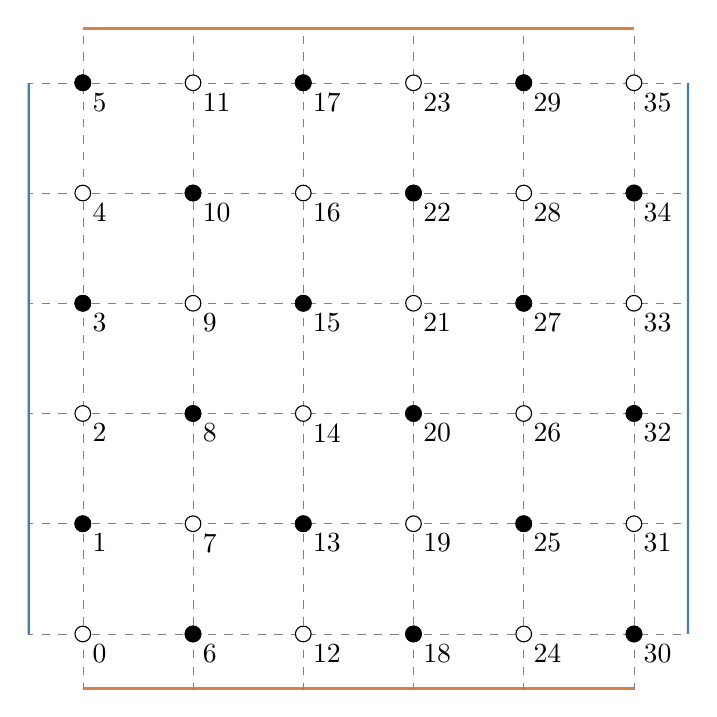
\begin{tikzpicture}[scale = 0.7]

    \clip (-1.0,-1.0) rectangle (11.0cm,11.0cm); % Clips the picture...
	\draw [ultra thick,sciBlue] (-1.0,-0.0)
        -- (-1.0cm,10.0cm) node [below left] {};
	\draw [ultra thick,sciOrange] (-0.0,-1.0)
        -- (10.0cm,-1.0cm) node [below left] {};

	\draw [ultra thick,sciBlue] (11.0,-0.0)
        -- (11.0cm,10.0cm) node [below left] {};
	\draw [ultra thick,sciOrange] (-0.0,11.0)
        -- (10.0cm,11.0cm) node [below left] {};
        
        
    \coordinate (Origin)   at (2,4);
    \coordinate (R)   at (4,4);
    \coordinate (U)   at (2,6);
    \coordinate (RU)   at (4,6);
    \coordinate (D)   at (2,2);
    \coordinate (RD)   at (4,2);
    \draw[style=help lines,dashed] (-14,-14) grid[step=2cm] (14,14);

      \foreach \x in {-7,-6,...,7}{% Two indices running over each
      \foreach \y in {-7,-6,...,7}{% node on the grid we have drawn 
        \node[draw,circle,inner sep=2pt,fill = white] at (2*\x,2*\y) {};		
        \pgfmathsetmacro{\z}{int(6*\x+\y)}
        \node[below right] at (2*\x,2*\y) {\z};
            % Places a dot at those points
      }
    }              
              
    
 
    \foreach \x in {-7,-5,...,6}{% Two indices running over each
      \foreach \y in {-6,-4,...,6}{
        \node[draw,circle,inner sep=2pt,fill] at (2*\x,2*\y) {};
      }
    }
    \foreach \x in {-6,-4,...,6}{% Two indices running over each
      \foreach \y in {-7,-5,...,6}{
        \node[draw,circle,inner sep=2pt,fill] at (2*\x,2*\y) {};
      }
    }

    

  \end{tikzpicture}
  \caption[Lattice representation]{Every point on the lattice is given a unique index, shared across every process. White and black dots represent sites of even and odd parity respectively, the relevance of this is explained in section \ref{sec:Checkerboard_Update}. Edges associated by periodic boundary conditions are denoted by coloured lines.}
  \label{figure:global_index}
\end{figure}





\section{Parallelization}\label{sec:parallelization}
LQCD is inherently very costly to simulate, and the cost increases rapidly for the larger lattices required to maintain the simulation volume at small lattice spacings. Therefore it is a necessity that the program includes some form of parallel computing, specifically the type known as "Single instruction, multiple data" or SIMD. To do this, the simulation volume is split into a number of non-overlapping areas of responsibility, each assigned to a different process. A popular protocol for handling cross- process communications, timing, I/O and many other features, is known as MPI (Message-Passing-Interface), and it's the protocol this program is based on.\\\\Every process will have two sets of sites in its memory which we may call "sites of responsibility" and "boundary sites". The former are all the sites which that process will have the sole responsibility for updating. The latter are all the sites which the process needs in order to complete its calculations, but which are within another process' sites of responsibility. The scope of boundary sites required by a process is dependent on the type of operations it's required to do. For example, calculating the plaquette term in the Wilson action requires only the first layer of boundary sites. More complicated terms, such as the clover terms in our definition for the lattice field strength tensor  illustrated in figure \ref{fig:Clovers}, requires three layers of boundary sites.\\\\We'll want a set of indices unique to each process, this is mainly for two reasons: data locality and keeping indices going from zero and up.
We can imagine trying to use the set of global indices to index a list of field values. When the program is updating a point on the lattice, it will need to fetch the field values of the surrounding points from memory. If the data of those points are stored sequentially in memory, there is a chance that that data can be found in the cache, which is much greater if they are stored physically close in memory.\\With the global indices, this is very unlikely to happen as neighbouring points will be separated by many numbers corresponding to points outside the process domain. The local index is only assigned to points which are needed by the process, which keeps the separation in indices between neighbouring points low, and therefore the chance of cache hits high, improving performance.\\\\With this point in mind, another consideration is the fact that Monte Carlo updates with the local Wilson action only uses field values from points of opposite parity, which gives another point of improvement for the local index system. By first assigning indices to points of one parity, then the other, relevant field values are even more closely located in memory, improving caching even further. This local index system is illustrated in figure \ref{figure:Local_lattice_parameterization}.


\begin{figure}
  \centering
  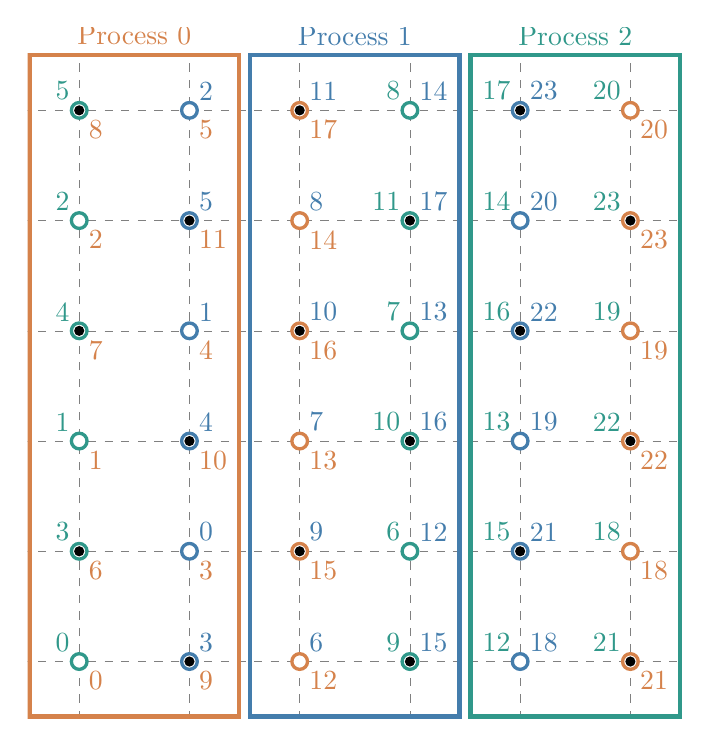
\begin{tikzpicture}[scale = 0.7]

    \clip (-0.935,-1.04) rectangle (10.95cm,11.5cm); % Clips the picture...
	

	
  \node[above] at (1,11) {\textcolor{sciOrange}{Process 0}};
  \node[above] at (5,11) {\textcolor{sciBlue}{Process 1}};
  \node[above] at (9,11) {\textcolor{sciGreen}{Process 2}};	
	
    \coordinate (Origin)   at (2,4);
    \coordinate (R)   at (4,4);
    \coordinate (U)   at (2,6);
    \coordinate (RU)   at (4,6);
    \coordinate (D)   at (2,2);
    \coordinate (RD)   at (4,2);
    \draw[style=help lines,dashed] (-14,-14) grid[step=2cm] (14,11);
	\draw[ultra thick,color = sciOrange] (-0.9,-1.0) rectangle (2.9,11.0);
	\draw[ultra thick,color = sciBlue] (3.1,-1.0) rectangle (6.9,11.0);
	\draw[ultra thick,color = sciGreen] (7.1,-1.0) rectangle (10.9,11.0);
	\foreach \x in {0,6}{
      \foreach \y in {-7,-6,...,7}{
        \node[draw = sciGreen,very thick,draw,circle,inner sep=2pt,fill = white] at (\x,2*\y) {};		
      }     
           
    } 
    
    	\foreach \x in {2,8}{
      \foreach \y in {-7,-6,...,7}{
        \node[draw = sciBlue,very thick,draw,circle,inner sep=2pt,fill = white] at (\x,2*\y) {};		
      }          
    } 
	\foreach \x in {4,10}{
      \foreach \y in {-7,-6,...,7}{
        \node[draw = sciOrange,very thick,draw,circle,inner sep=2pt,fill = white] at (\x,2*\y) {};		
      }          
    } 
    \foreach \x in {2,6,10}{
      \foreach \y in {-6,-4,...,6}{
        \node[fill,circle,very thick,inner sep=1.3pt,fill = black] at (\x,2*\y) {};		
      }          
    } 
        \foreach \x in {0,4,8}{
      \foreach \y in {-7,-5,...,7}{
        \node[fill,circle,very thick,inner sep=1.3pt,fill = black] at (\x,2*\y) {};		
      }          
    } 
    

  \node[below right] at (0,0) {\textcolor{sciOrange}{0}};
  \node[below right] at (0,4) {\textcolor{sciOrange}{1}};
  \node[below right] at (0,8) {\textcolor{sciOrange}{2}};
  \node[below right] at (2,2) {\textcolor{sciOrange}{3}};
  \node[below right] at (2,6) {\textcolor{sciOrange}{4}};
  \node[below right] at (2,10) {\textcolor{sciOrange}{5}};
  \node[below right] at (0,2) {\textcolor{sciOrange}{6}};
  \node[below right] at (0,6) {\textcolor{sciOrange}{7}};
  \node[below right] at (0,10) {\textcolor{sciOrange}{8}};
  \node[below right] at (2,0) {\textcolor{sciOrange}{9}};
  \node[below right] at (2,4) {\textcolor{sciOrange}{10}};
  \node[below right] at (2,8) {\textcolor{sciOrange}{11}};
  \node[below right] at (4,0) {\textcolor{sciOrange}{12}};
  \node[below right] at (4,4) {\textcolor{sciOrange}{13}};
  \node[below right] at (4,8) {\textcolor{sciOrange}{14}};
  \node[below right] at (4,2) {\textcolor{sciOrange}{15}};
  \node[below right] at (4,6) {\textcolor{sciOrange}{16}};
  \node[below right] at (4,10) {\textcolor{sciOrange}{17}};
  \node[below right] at (10,2) {\textcolor{sciOrange}{18}};
  \node[below right] at (10,6) {\textcolor{sciOrange}{19}};
  \node[below right] at (10,10) {\textcolor{sciOrange}{20}};
  \node[below right] at (10,0) {\textcolor{sciOrange}{21}};
  \node[below right] at (10,4) {\textcolor{sciOrange}{22}};
  \node[below right] at (10,8) {\textcolor{sciOrange}{23}};
  
  \node[above right] at (2,0) {\textcolor{sciBlue}{3}};
  \node[above right] at (2,4) {\textcolor{sciBlue}{4}};
  \node[above right] at (2,8) {\textcolor{sciBlue}{5}};
  \node[above right] at (4,2) {\textcolor{sciBlue}{9}};
  \node[above right] at (4,6) {\textcolor{sciBlue}{10}};
  \node[above right] at (4,10) {\textcolor{sciBlue}{11}};
  \node[above right] at (2,2) {\textcolor{sciBlue}{0}};
  \node[above right] at (2,6) {\textcolor{sciBlue}{1}};
  \node[above right] at (2,10) {\textcolor{sciBlue}{2}};
  \node[above right] at (4,0) {\textcolor{sciBlue}{6}};
  \node[above right] at (4,4) {\textcolor{sciBlue}{7}};
  \node[above right] at (4,8) {\textcolor{sciBlue}{8}};
  \node[above right] at (6,0) {\textcolor{sciBlue}{15}};
  \node[above right] at (6,4) {\textcolor{sciBlue}{16}};
  \node[above right] at (6,8) {\textcolor{sciBlue}{17}};
  \node[above right] at (6,2) {\textcolor{sciBlue}{12}};
  \node[above right] at (6,6) {\textcolor{sciBlue}{13}};
  \node[above right] at (6,10) {\textcolor{sciBlue}{14}};
  \node[above right] at (8,2) {\textcolor{sciBlue}{21}};
  \node[above right] at (8,6) {\textcolor{sciBlue}{22}};
  \node[above right] at (8,10) {\textcolor{sciBlue}{23}};
  \node[above right] at (8,0) {\textcolor{sciBlue}{18}};
  \node[above right] at (8,4) {\textcolor{sciBlue}{19}};
  \node[above right] at (8,8) {\textcolor{sciBlue}{20}};
  
  \node[above left] at (0,0) {\textcolor{sciGreen}{0}};
  \node[above left] at (0,4) {\textcolor{sciGreen}{1}};
  \node[above left] at (0,8) {\textcolor{sciGreen}{2}};
  \node[above left] at (6,0) {\textcolor{sciGreen}{9}};
  \node[above left] at (6,4) {\textcolor{sciGreen}{10}};
  \node[above left] at (6,8) {\textcolor{sciGreen}{11}};
  \node[above left] at (0,2) {\textcolor{sciGreen}{3}};
  \node[above left] at (0,6) {\textcolor{sciGreen}{4}};
  \node[above left] at (0,10) {\textcolor{sciGreen}{5}};
  \node[above left] at (6,2) {\textcolor{sciGreen}{6}};
  \node[above left] at (6,6) {\textcolor{sciGreen}{7}};
  \node[above left] at (6,10) {\textcolor{sciGreen}{8}};
  \node[above left] at (8,2) {\textcolor{sciGreen}{15}};
  \node[above left] at (8,6) {\textcolor{sciGreen}{16}};
  \node[above left] at (8,10) {\textcolor{sciGreen}{17}};
  \node[above left] at (8,0) {\textcolor{sciGreen}{12}};
  \node[above left] at (8,4) {\textcolor{sciGreen}{13}};
  \node[above left] at (8,8) {\textcolor{sciGreen}{14}};
  \node[above left] at (10,0) {\textcolor{sciGreen}{21}};
  \node[above left] at (10,4) {\textcolor{sciGreen}{22}};
  \node[above left] at (10,8) {\textcolor{sciGreen}{23}};
  \node[above left] at (10,2) {\textcolor{sciGreen}{18}};
  \node[above left] at (10,6) {\textcolor{sciGreen}{19}};
  \node[above left] at (10,10) {\textcolor{sciGreen}{20}};

      
  \end{tikzpicture}
  \caption[Lattice partitioning]{The lattice is partitioned into 3 processes whose sites of responsibility are enclosed within their respective coloured rectangle. Each process reserves memory for every site contained within its domain of responsibility in addition to the sites encircled with the color belonging to that process.\\Every process maintains its own internal parametrization of the lattice given by indices assigned from zero, to the total number of sites stored by that process, with the following precedence: sites of lowest process rank $\rightarrow$ sites of even parity $\rightarrow$ sites of odd parity.}
  \label{figure:Local_lattice_parameterization}
\end{figure}
\subsection{Lattice Partitioning}
The lattice can be subdivided among processes in many different ways. The two methods that have been implemented are working within a few constraints: limiting the size of communications and the number of different processes neighbouring each process, packing as many processes onto the lattice as possible and partitioning equally many points to every process. This is to reduce communication overhead, improve parallellization scaling and reduce thread downtime respectively.\\\\We can roughly approximate the communication overhead as being proportional to the amount of data being shared between processes (within some hardware imposed threshold) and as scaling with some function of the number of different processes each process needs to establish communication with. The size of transferred data packets can be reduced by e.g. using a checkerboard update and only communicating sites of a given parity. We can also improve efficiency through how we partition the lattice among processes.\\\\Working in four dimensions and using only boxes which evenly divide the lattice into $N_{procs}$ domains. Naively, we might think the problem of improving efficiency comes down to something like the following:
\begin{equation*}
\operatorname{min}\left\{  2(xyz + xyt + xtz + ytz) \,\Big|\,xyzt = \frac{|\Lambda|}{N_{procs}}\right\}
\end{equation*}
where we attempt to minimize the $(4-1)$-volume of the boundary between process domains and conclude that $x=y=z=t$. But this neglects a crucial detail of the lattice we actually want to implement: it has periodic boundary conditions. We see that the topology imposed on the lattice by the periodic boundary conditions alters the problem statement, because when a process' domains' extent in a dimension is the size of the lattice in that dimension, it will boarder itself in that dimension. This means that those boundary sites would no longer have to be communicated between processes. We get the following optimization problem:
\begin{equation*}
\begin{aligned}
\operatorname{min}\Big\{  &2(xyz\delta(t-|\Lambda_t|) + xyt\delta(z-|\Lambda_z|) + \\
 & xtz\delta(y-|\Lambda_y|) + ytz\delta(x-|\Lambda_x|)) \,\Big|\,xyzt = \frac{|\Lambda|}{N_{procs}} \Big\}
\end{aligned}
\end{equation*}

for 
\begin{equation*}
\delta(x) = \begin{cases}0 & \text { if }x=0 \\ 1 & \text { otherwise }\end{cases}.
\end{equation*}
and 
\begin{equation*}
x\leq|\Lambda_x|,\,y\leq|\Lambda_y|,\,z\leq|\Lambda_z|,\,t\leq|\Lambda_t|
\end{equation*}

Which choice of $x,\,y,\,z$ and $t$ minimize this expression turns out to be highly dependent on the ratio $\frac{|\Lambda|}{N_{procs}}$ and we can make sense of why that is. When the simulation volume of each process is small, the reduction in boundary 3-volume gained from setting any $x,\,y,\,z,\,t = |\Lambda_x|,\,|\Lambda_y|,\,|\Lambda_z|,\,\Lambda_t|$ is quite small, while the addition of boundary 3-volume by deviating from $x=y=z=t$ becomes quite large. Likewise, when each process' simulation volume is large, there is substantial reductions to be made from eliminating either of the terms in the above minimization problem.\\For instance, in many LQCD simulations the time extent of the lattice can be much larger than the spatial extent, and so all of the three terms that include $t$ could be completely removed by only subdividing the temporal dimension of the lattice, i.e. $x=|\Lambda_x|,\,y=|\Lambda_y|,\,z=|\Lambda_z|$.\\Another benefit of partitioning the lattice in this way is that there is a hardware-specific overhead associated with establishing communications between two processes, and eliminating process boundaries in a dimension will require fewer connections between processes.\\\\Ultimately this choice will depend on the number of processors that are available to you and the total simulation volume, as well as the relative difference in computer time associated with either establishing communications between processes or transceiving a certain amount of data between processes. Regardless, for all but the most modest core-counts, this minimization problem favours hyper-cubic process domains by a significant margin, especially when it comes to scaling, as subdivisions in more dimensions admit more processes to be used.\\\\But what if you had access to a specific amount of processors and you want to use as many of them as possible? If we ignore the issue of face elimination, which we tackled above, and restrict ourselves to 4 dimensional hyper-cubic latices $\Lambda_x=\Lambda_y=\Lambda_z=\Lambda_t$ (this isn't necessary, but it makes the equations easier to work with) we can look at the demands this way: $\Lambda_x$ must be divisible by the number of "cuts" $n^\mu_c$ in that dimension and 
\begin{equation}
(n^0_c+1)(n^1_c+1)(n^2_c+1)(n^3_c+1)= N_{procs}.
\end{equation}
Where $N_{procs}$ is the number of processors available to you. It can be solved by an algorithm like the one in listings \ref{alg:Create_partition}.\\Once the number of cuts $n_c^\mu$ has been decided from the list output by \ref{alg:Create_partition}, the lattice is then partitioned based on the algorithm in listing \ref{alg:Partition_Lattice}.
\begin{algorithm}
\caption{Create Partition}\label{alg:Create_partition}
\hspace*{\algorithmicindent} \textbf{Input: $N_{procs}$, $\Lambda_x$} \\
\hspace*{\algorithmicindent} \textbf{Output: $n^0_c$, $n^1_c$, $n^2_c$, $n^3_c$, $N^{usable}_{procs}$}
\begin{algorithmic}
\State $n^0_c,\,n^1_c,\,n^2_c,\,n^3_c$
\For{$n^0_c,\,n^1_c,\,n^2_c,\,n^3_c \,\forall$ combinations of divisors of $\Lambda_x$ with replacement $-1$}
\If{$(n^0_c+1)(n^1_c+1)(n^2_c+1)(n^3_c+1) = N^{usable}_{procs} \leq N_{procs}$}
\State append $n^0_c,\,n^1_c,\,n^2_c,\,n^3_c$ and $N^{usable}_{procs}$ to output
\EndIf
\EndFor

\end{algorithmic}
\end{algorithm}


\begin{algorithm}
\caption{Partition lattice}\label{alg:Partition_Lattice}
\hspace*{\algorithmicindent} \textbf{Input: $n^0_c$, $n^1_c$, $n^2_c$, $n^3_c$}
\begin{algorithmic}
\Ensure
\State $proc_{id} = 0$
\For{$\forall\,\vec{n} \in \Lambda$}

\For{$i \in \{0,1,\ldots,N_{dims}\}$}
x\State $temp \gets \vec{n}_i/(\Lambda_i/n^i_c+1)$
\For{$j<i$}
\State $temp \gets temp\cdot(n^j_c+1)$
\EndFor
\State $proc_{id} \gets proc_{id}+ temp$
\EndFor
\State \Return Process id of $\vec{n}$ is $proc_{id}$
\State $proc_{id}\gets 0$
\EndFor

\end{algorithmic}
\end{algorithm}

\subsection{Checkerboard Update}\label{sec:Checkerboard_Update}
Applying parallelization to the updating of link variables presents an issue. When a link is being updated it is necessary to ensure that none of the links required for its calculation are changed until the calculation is concluded.\\For the Wilson action, the set of links required to update a link are the links contained in the staples connected to it. One way to ensure that this requirement is met, is to assign to each lattice point either an even or odd parity according to its coordinate
such that 
\begin{equation}
parity(\mathbf{x}) = \left( \sum\limits_i x_i \right) \mod 2.
\end{equation}
Then by choosing either parity $0$ or $1$ and a direction $\mu$, every such link variable can be simultaneously updated without impacting each other. This ends up looking, for a two- dimensional slice of the four- dimensional lattice, as illustrated in figure \ref{figure:Even-Odd}
\begin{figure}
  \centering
  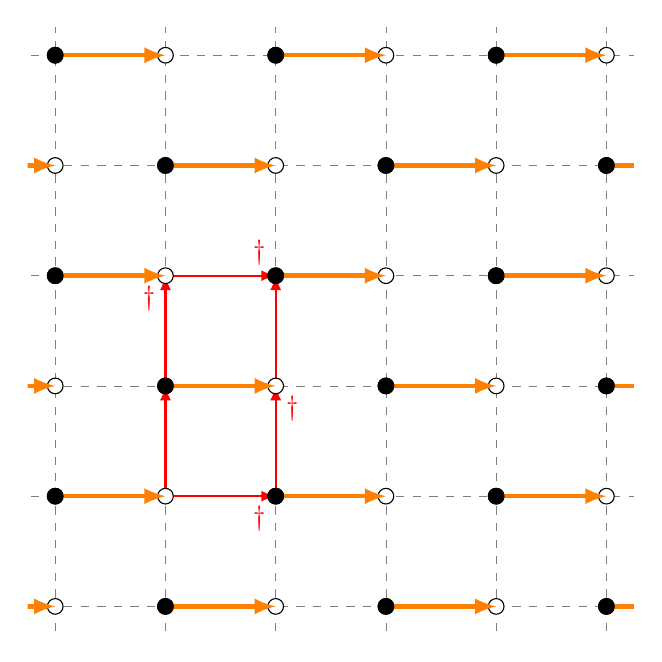
\begin{tikzpicture}[scale = 0.7]

    \clip (-0.5,-0.5) rectangle (10.5cm,10.5cm); % Clips the picture...

    \coordinate (Origin)   at (2,4);
    \coordinate (R)   at (4,4);
    \coordinate (U)   at (2,6);
    \coordinate (RU)   at (4,6);
    \coordinate (D)   at (2,2);
    \coordinate (RD)   at (4,2);
    \draw[style=help lines,dashed] (-14,-14) grid[step=2cm] (14,14);
          % Draws a grid in the new coordinates.
          %\filldraw[fill=gray, fill opacity=0.3, draw=black] (0,0) rectangle (2,2);
              % Puts the shaded rectangle
    \draw [thick,-latex,red] (R)
        -- (RU) node [below right] {};   
    \draw [thick,-latex,red] (U)
        -- (RU) node [above left] {$\dagger$};    
    \draw [thick,-latex,red] (Origin)
        -- (U) node [below left] {$\dagger$}; 
    \draw [thick,-latex,red] (RD)
        -- (R) node [below right] {$\dagger$};   
    \draw [thick,-latex,red] (D)
        -- (RD) node [below left] {$\dagger$};    
    \draw [thick,-latex,red] (D)
        -- (Origin) node [below left] {}; 
        \foreach \x in {-7,-6,...,7}{% Two indices running over each
      \foreach \y in {-7,-6,...,7}{% node on the grid we have drawn 
        \node[draw,circle,inner sep=2pt,fill = white] at (2*\x,2*\y) {};
            % Places a dot at those points
      }
    }              
              
    
 
    \foreach \x in {-7,-5,...,6}{% Two indices running over each
      \foreach \y in {-6,-4,...,6}{% node on the grid we have drawn 
              \draw [ultra thick,-latex,orange] (2*\x,2*\y)
        -- (2*\x+2,2*\y) node [below left] {};
        \node[draw,circle,inner sep=2pt,fill] at (2*\x,2*\y) {};

            % Places a dot at those points
      }
    }
    \foreach \x in {-6,-4,...,6}{% Two indices running over each
      \foreach \y in {-7,-5,...,6}{% node on the grid we have drawn 
              \draw [ultra thick,-latex,orange] (2*\x,2*\y)
        -- (2*\x+2,2*\y) node [below left] {};
        \node[draw,circle,inner sep=2pt,fill] at (2*\x,2*\y) {};

            % Places a dot at those points
      }
    }

    

  \end{tikzpicture}
  \caption[Checkerboard update]{Choosing a site parity and a direction $\mu$, every link $U_\mu (x_{parity})$ can be independently updated without affecting links relevant to the computation of any other $U_\mu (x_{parity})$. }
  \label{figure:Even-Odd}
\end{figure}

We see that the lattice must necessarily contain an even number of sites in every direction in order for the lattice to be correctly partitioned into even and odd sites for periodic boundary conditions.

\subsection{Field communication}
All communication between processes is done using MPI. MPI provides a few different standards for doing this, which influences its behaviour. There are many such standards but most simply, there are so-called 'blocking' and 'non-blocking' variants. A blocking send command is called using $MPI\_Send()$. This will transfer a buffer to the specified process, then wait for confirmation from the receiving process before moving on. This is quite bad for performance, because the receiving process might be farther behind in its computations, halting the sending process until it is ready to receive.\\Rather than doing this, we use the non-blocking variant which is called using $MPI\_ISend()$. This command will send the buffer, then immediately move on to the next lines of code. This allows the sending process to execute code until it's halted by a $MPI\_Wait()$ command at which point, it waits for confirmation from the receiving process before moving on.\\This distinction is quite important, because it allows the process to spend that extra time receiving data from yet another process. The ids' of the process which is sent to and received from is determined by
\begin{equation}
Id_{send\,to} = \operatorname{mod}(id + i,N_{procs}),\,\,i \in \{ 1,\ldots,N_{procs}-1 \}
\end{equation}
\begin{equation}
Id_{rec\,from} = \operatorname{mod}(id + N_{procs} - i,N_{procs}),\,\,i \in \{ 1,\ldots,N_{procs}-1 \}
\end{equation}

\chapter{Results}

\section{Improved v. clover- Field strength tensor}
We had different choices for which lattice field strength tensor definition to use, so it's obviously interesting to see what effect it had. Because the analysis only included one of the definitions, this is a rather limited analysis, performed at the very last point along the flow, where the whole gauge configurations had been saved, rather than just the observables. Still, we can try to glean some information from this.\\\\We see from figure \ref{fig:Q_FST_defs_diff} that the clover definition of the topological charge produces results which differ substantially from the improved definition. The clover definition of the lattice field strength tensor produces a topological charge definition with $\mathcal{O}(a^2)$ errors compared to the $\mathcal{O}(a^4)$ errors arising from the improved definition. The implications this has for the measured value of the topological susceptibility is analysed in section \ref{sec:universalityOfDef}.\\\\
\begin{figure}[htbp]
\centering
\includegraphics[width=0.7\textwidth]{FINALPLOTS/Q_def_diff.pdf}
\caption[]{Expectation value of the difference between the two topological charge definitions when measuring the same configuration. The measurements are taken at $t/a^2 = \{13,\,8.5,\,5.5,\,3.5 \}$ from left to right.}\label{fig:Q_FST_defs_diff}
\end{figure}
For the energy density we see that the ratios of the improved- and clover- definitions produce a roughly linear relationship in $\frac{a^2}{r_0^2}$.  It's noticeable that the coarsest lattice produces considerably larger differences than the finer lattices. This observation will inform our analysis of $\Lambda_{YM}$- scale.
\begin{figure}[htbp]
\centering
\includegraphics[width=0.7\textwidth]{FINALPLOTS/E_def_diff.pdf}
\caption[]{Ratios of the expectation values of the two Energy density definitions ((I)mproved \& (C)lover) when measuring the same configurations. The measurements are taken at $t/a^2 = \{13,\,8.5,\,5.5,\,3.5 \}$ from left to right.}\label{fig:E_FST_defs_diff}
\end{figure}
\FloatBarrier
\section{Energy density}
The Wilson flow drives the action towards its stationary points. We therefore expect the energy density of the gauge field to go to zero in the large flow time limit. This is exactly what we find, as can be seen in figure \ref{fig:EvFlow}. 
\begin{figure}[htbp]
\centering
\includegraphics[width=0.7\textwidth]{FINALPLOTS/E_v_flowtime.pdf}
\caption[]{Expectation value of the energy density as a function of the physical flow time over the square of the Sommer parameter. The error bars are smaller than the symbols. }\label{fig:EvFlow}
\end{figure}
\subsection{Scale setting with $t^2\langle E\rangle$}
As we saw, to leading order in perturbation theory, $t^2\langle E\rangle$ is proportional to the gauge coupling. We expect that this perturbative expansion should match our lattice results within some range of flow times. This is between the range in which perturbation theory is expected to break down and where the discretization effects of the lattice causes scaling violations in $\langle E\rangle$.\\In figure \ref{fig:tsquaredE_v_flowtime}, which has been replicated from Lüscher's paper\cite{Luscher2010}, we see that the finest lattice produces near perfect agreement with perturbation theory within the range of roughly $\frac{t}{r_0^2}=0.01$ to $\frac{t}{r_0^2}=0.035$. This region corresponds to a smearing radius $\sqrt{8t}$ which is $3-5.6$ times the lattice spacing.
\begin{figure}[htbp]
\centering
\includegraphics[width=0.7\textwidth]{FINALPLOTS/t_squared_v_tOverR_0_squared.pdf}
\caption[]{The dimensionless combination $t^2\langle E\rangle$ as a function of the physical flow time over the squared Sommer radius. The errorband in the perturbative expansion is dominated by the uncertainty in $\Lambda\big|_{N_f=0}$ which is sited in \cite{CapitaniStefano1999Nqmr}. The errorbars are not visible on the scale of the figure.}\label{fig:tsquaredE_v_flowtime}
\end{figure}
In the same paper, Lüscher proposed the introduction of a reference scale $t_0$ defined by the implicit equation \eqref{eq:t0RefImplicitEq}. We can identify $\frac{t_0}{r_0^2}$ by the point in figure \ref{fig:tsquaredE_v_flowtime} at which the graph crosses $t^2\left\langle E\right\rangle = 0.3$. We have a limited flow-time resolution, and so in order to get an estimate we have to interpolate between the points in its vicinity. We see the result of this extrapolation in figure \ref{fig:t0-extrapolation}. The error in $\frac{t_0}{r_0^2}$ comes from the uncertainty in $\frac{a}{r_0}$ as well as the statistical error in $t^2\left\langle E\right\rangle$. The systematic error arising from the interpolation is negligible. The estimate for every lattice spacing is consistent within errors.
\begin{figure}[htbp]
\centering
\includegraphics[width=0.7\textwidth]{FINALPLOTS/t0_extrapolate_with_errors.pdf}
\caption[]{Interpolation of the flow time dependence of $t^2\left\langle E\right\rangle $ in the vicinity of $\frac{t_0}{r_0^2}$. The interpolation includes the two points closest to the final answer. The vertical uncertainty derives from the uncertainty in $\frac{a}{r_0}$, while the horizontal uncertainty is the statistical error in $t^2\left\langle E\right\rangle $.}\label{fig:t0-extrapolation}
\end{figure}
We can see from figure \ref{fig:SmearRad_v_latticeConstant} that the discretization effects are much smaller than the errors. The discretization effect in this case, would manifest itself as a slope in the linear extrapolation in $\frac{a^2}{t_0}$, as the effective field theory using the Wilson action predicts dicretization effects of $\mathcal{O}(a^2)$. The continuum extrapolation of $\frac{\sqrt{8t_0}}{r_0}$ indicates very strongly that the dimensionless ratio $\frac{t_0}{r_0^2}$ is independent of the lattice spacing. The continuum value of $\frac{\sqrt{8t_0}}{r_0}$ is seen to extrapolate to
\begin{equation}
\frac{\sqrt{8t_0}}{r_0} = 0.943(6)
\end{equation}
which is in near perfect agreement with the result stated in \cite{non_gaussianities2015} of $\frac{\sqrt{8t_0}}{r_0} = 0.941(7)$. This result is from a very high statistics study using the same definition for the energy density, but at larger lattice spacings of $a = 0.102,\,0.087,\,0.077$ and $0.068fm$. The smaller extrapolation error incurred by having smaller lattice spacings, may be enough to explain the roughly equal magnitudes of the errors. As stated in their paper, the error in $\frac{\sqrt{8t_0}}{r_0}$ is dominated by the uncertainty in $\frac{a}{r_0}$ which is also the case here, meaning the higher statistics eventually saturates below the uncertainty of $\frac{a}{r_0}$, leaving the error roughly unchanged.
\begin{figure}[htbp]
\centering
\includegraphics[width=0.7\textwidth]{FINALPLOTS/smearRad_cont_limit.pdf}
\caption[]{Linear extrapolation in $a^2/t_0$ of $\frac{\sqrt{8t_0}}{r_0}$ to the continuum. The horizontal error is not visible on the scale of the figure.}\label{fig:SmearRad_v_latticeConstant}
\end{figure}

\subsection{Estimating $\Lambda_{YM}$}
Because the lattice results and the perturbative expansion match over a range of flow times, we can actually get an estimate for the YM-scale $\Lambda_{YM}$ through their relation in equations \eqref{eq:leadingOrder_pt_E} and \eqref{eq:runningCouplingApprox}. To do this, we have to exercise a fair bit of caution, as the range over which these results can be said to match, has no objective boundaries. If we were to base this analysis on the entirely subjective matching region discussed earlier, we might conclude that the results should match from approximately $q = 750-1400MeV$ where $q=\frac{1}{\sqrt{8t}}$ is the momentum scale as defined through equation \eqref{eq:runningCouplingApprox}\footnote{The gradient flow averages the gauge field in a spherical range with mean-square radius $\sqrt{8t}$, making the characteristic wavelength of the lattice $\frac{1}{\sqrt{8t}}$. This is quite reminiscent of how the RG-flow integrates out degrees of freedom.}. To make the analysis less biased, we'll instead consider a larger matching region of $q = 527-2358MeV$.\\\\Firstly, we need to extrapolate $t^2\left\langle E\right\rangle $ to the continuum over the range of flow times considered. As with the extrapolation of $t_0$, we now need to extrapolate a value of $t^2\left\langle E\right\rangle $ for several flow times between measurements. Again, this was done by interpolating between two subsequent datapoints. Then we perform the extrapolation to the continuum linearly in $\frac{a^2}{r_0^2}$.  At this point, the ensemble with the coarsest lattice spacing was excluded from the analysis. As we saw in figure \ref{fig:E_FST_defs_diff}, the difference from the improved definition becomes quite large which has big implications for the quality of the fit. The result of this continuum extrapolation is found in figure \ref{fig:Coupling_cont_extrapolation}.
\begin{figure}[htbp]
\centering
\includegraphics[width=0.7\textwidth]{FINALPLOTS/t_squared_v_q_contLimit.pdf}
\caption[]{$t^2\left\langle E\right\rangle $ dependence on the momentum scale $q = \frac{1}{\sqrt{8t}}[MeV]$ with the extrapolation to the continuum based on the three finest lattice spacings.}\label{fig:Coupling_cont_extrapolation}
\end{figure}
The continuum extrapolation contains a total of 100 points evenly spaced in $\frac{t}{r_0^2}$. To estimate $\Lambda_{YM}$, we proceed by resampling the set of 100 points by performing a $\chi^2$ fit of the function \eqref{eq:leadingOrder_pt_E} to every set of subsequent points with a length greater than or equal to 5. This is done until the list of possible resamples is exhausted and every examined value of $\Lambda_{YM}$ is assigned a score based on how well it fitted the data in every resample. When this is done, the results are as seen in figure \ref{fig:YM-Scale_chiSquaredFit}. This result is compatible with the result of $\Lambda^{(0)}_{MS} = 238(19)MeV$ from \cite{CapitaniStefano1999Nqmr}. I cannot de-emphasize the results of this analysis enough though. In order to sample the $400$ different values of $\Lambda_{YM}$, I've had to compromise away any analysis of the statistical error in the estimate, as any bootstrap sampling would take far to long execute. Sampling more values of $\Lambda_{YM}$ was seen to have a very large impact on the final result as lowering the sample rate had a tendency to exclude highly weighted values, deforming the result. I should also make a note of a very important detail which was glossed over in the introduction to this analysis. This detail is immediately apparent, looking at figure \ref{fig:Coupling_cont_extrapolation}: we chose to space the values evenly in $\frac{t}{r_0^2}$, not in $\frac{1}{\sqrt{8t}}$. This has the effect of weighting the points in the lower energy region much higher than those in the high energy region. Doing the exact same analysis, now with the samples being evenly spaced in $\frac{1}{\sqrt{8t}}$, we get the result in figure \ref{fig:YM-Scale_chiSquaredFit-altspac} .
This result is a very strong signal that we don't have our systematic errors under control.\\This being said, there are genuine reasons for why we might want to weight lower energies more than higher energies, such as the fact that the low flow time extrapolations don't have a well defined continuum limit. 


\begin{figure}[htbp]
\centering
\includegraphics[width=0.7\textwidth]{FINALPLOTS/t_squared_v_q_ChiSquared_fitDistribution_HIST.pdf}
\caption[]{Weighted distribution of $\Lambda_{YM}$ fitting equation \eqref{eq:leadingOrder_pt_E} to the resamples of the continuum extrapolation of $t^2\left\langle E\right\rangle $ using the 4-loop approximation of the running coupling found in equation \eqref{eq:runningCouplingApprox}. The three vertical lines denote the weighted median and its $68\%$ confidence interval which are $224.96MeV$, $234.59MeV$ and $240.15MeV$ from left to right. The peak corresponds to a value of $237.74MeV$.}\label{fig:YM-Scale_chiSquaredFit}
\end{figure}

\begin{figure}[htbp]
\centering
\includegraphics[width=0.7\textwidth]{FINALPLOTS/t_squared_v_q_ChiSquared_fitDistribution-altSpacing.pdf}
\caption[]{Weighted distribution of $\Lambda_{YM}$ fitting equation \eqref{eq:leadingOrder_pt_E} to the resamples of the continuum extrapolation of $t^2\left\langle E\right\rangle $ using the 4-loop approximation of the running coupling found in equation \eqref{eq:runningCouplingApprox}. Fitting done on values separated evenly in $\frac{1}{\sqrt{8t}}$}\label{fig:YM-Scale_chiSquaredFit-altspac}
\end{figure}
\FloatBarrier
\section{Topological charge}
Recalling our discussion of the separation of topological sectors in section \ref{sec:sepofTopSec} and the set of gauge fields which satisfy the smoothness bound encoded by equation \eqref{eq:actionDensityExpVal}; we can now finally see the implications of these facts manifest themselves in the flow time behaviour of the topological charge on lattices of different lattice spacings. What we expect to see at this point, is that as the set of gauge configurations satisfying the smoothness bound goes to one, i.e. by decreasing the lattice spacing, more and more gauge configurations should settle into integer values of the topological charge, earlier in the gradient flow. This fact is also clear from the functional integral in \eqref{eq:flowTimeFunctionalIntegral}, where the $t-$ and $a-$ dependence of the transformed action weights configurations with a well defined topological charge (near integer values) more than configurations with a poorly defined topological charge (deviations from integer values). This behaviour is clearly evident in figure \ref{fig:QvFlowTime}, where gauge configurations of smaller lattice spacings can be seen to saturate at near- integer values, earlier in the flow time.
\begin{figure}[htbp]
\centering
\includegraphics[width=0.7\textwidth]{FINALPLOTS/Q_v_flowtime.pdf}
\caption[]{Flow time dependence of the topological charge going from coarsest to finest lattice spacing from top to bottom. $\frac{t_0}{a^2}$ corresponds to the computer- flow time at which the topological susceptibility is measured. 21 samples of each ensemble are illustrated.}\label{fig:QvFlowTime}
\end{figure}
A very interesting behaviour can be seen to occur in the flow time dependence of the topological charge in the $\beta = 6.26$ ensemble\footnote{This behaviour has been seen in all three of the coarsest lattice spacings, but are not illustrated here.}. One of the gauge configurations which had seemingly settled into a near-integer value, proceeds to deviate from that integer value. Continuing the flow on one of these configuration eventually leads to the topological charge settling into a new integer value. I have no firm explanation for this phenomenon other than to conjecture that the flow equations briefly trap the gauge field in a region of small gradient. The deviation seems to appear when the smearing radius $\sqrt{8t}$ is close to $\frac{1}{3}L$ indicating that the averaging procedure eventually pushes the gauge configuration out of the local minimum. To test this, we could examine many such configurations to see whether the frequency of such occurrences go to zero as $\sqrt{8t}\rightarrow L$.\\\\Next we make a qualitative analysis of the flow time dependence of the distribution of topological charge density on the lattice. We can look at the gradient flow as cooling the short range fluctuations in the field configurations, revealing the underlying topological structure.
Figure \ref{fig:Qdensdist_all} illustrates this procedure for a 3D euclidean time slice of the full space-time lattice on a gauge configuration with the finest lattice spacing and a topological charge of $4$ in the large flow time limit.\\\\At flow times close to zero, we find exactly what we expect, large short range fluctuations which obscure any real structure. It's only at $\frac{t}{a^2}\approx 1.21$ that we begin to see some structure in the local fluctuations. Curiously, at this stage the topological charge has nearly settled into its final value. Seeing just how little resemblance this distribution has to the final distribution at $\frac{t}{a^2}=13$ with only a slightly higher topological charge is noteworthy. At large flow times, we see the topological charge density settle into 'lumps' which are exclusively positive or negative, separated by regions of zero topological charge density. These are the localised instanton solutions to the Wilson action each with an associated 'winding'-number.


\begin{figure}[htbp]
\centering
\begin{subfigure}{0.5\textwidth}
\centering
\includegraphics[trim=30cm 0.0cm 27cm 2.0cm, clip=true,width=\linewidth]{FINALPLOTS/QdensityPlots/3D/vFlowTime/torus_extdof1_44_Flowtime0.010000.pdf}
\caption{$\frac{t}{a^2} = 0.01$. $Q \approx -8.7 $}\label{fig:Qdensdist1}
\end{subfigure}%
\begin{subfigure}{0.5\textwidth}
\centering
\includegraphics[trim=30cm 0.0cm 27cm 2.0cm, clip=true,width=\linewidth]{FINALPLOTS/QdensityPlots/3D/vFlowTime/torus_extdof1_44_Flowtime0.410000.pdf}
\caption{$\frac{t}{a^2} = 0.41$. $Q \approx 3.52 $}\label{fig:Qdensdist2}
\end{subfigure}
\begin{subfigure}{0.5\textwidth}
\centering
\includegraphics[trim=30cm 0.0cm 27cm 2.0cm, clip=true,width=\linewidth]{FINALPLOTS/QdensityPlots/3D/vFlowTime/torus_extdof1_44_Flowtime1.210000.pdf}
\label{fig:Qdensdist3}
\caption{$\frac{t}{a^2} = 1.21$. $Q \approx 3.99 $}
\end{subfigure}%
\begin{subfigure}{0.5\textwidth}
\centering
\includegraphics[trim=30cm 0.0cm 27cm 2.0cm, clip=true,width=\linewidth]{FINALPLOTS/QdensityPlots/3D/vFlowTime/torus_extdof1_44_Flowtime13.000000.pdf}
\label{fig:Qdensdist4}
\caption{$\frac{t}{a^2} = 13.0$. $Q = 3.99996$}
\end{subfigure}
\caption[]{Topological charge distribution at euclidean time slice $t_{euc}=0$ measured at different flow times. Generated using the Mayavi python plotting utility \cite{ramachandran2011mayavi}. The star shape is only an artefact of the 2D projection.}
\label{fig:Qdensdist_all}
\end{figure}


\FloatBarrier
\section{Topological susceptibility}
We begin the study of the topological susceptibility by examining its flow time dependence. In figure \ref{fig:FlowTime_v_smearRad}, we plot the fourth root of the topological susceptibility in physical units as a function of the dimensionless ratio $\frac{\sqrt{8t}}{r_0}$. We can see that the topological susceptibility at $\frac{\sqrt{8t}}{r_0}=0$ is dominated by ultraviolet fluctuations. Because the lattice constant acts as an ultraviolet cut-off, when the lattice spacing is decreased i.e. the cut-off is removed, the ultraviolet divergences become more severe. In figure \ref{fig:ZeroFlowTime_chifourthroot}, this behaviour of the topological susceptibility at flow time $t=0$ is evident when compared to the values measured at flow time $t=t_0$. This behaviour is evident from the definition in equation \eqref{eq:flowtimeChiDef}
\begin{equation}\label{eq:flowtimeChiDef}
\chi_{\mathrm{t}}=\frac{1}{V} \int d^{4} x d^{4} y\left\langle q(x) q(y)\right\rangle\big|_{U(t)}
\end{equation}
where the contact term (moderated by the minimally allowed lattice distance $a$) induces a $1/a^4$ divergence in the topological susceptibility. This shows up as the $\frac{a^2}{r_0^2}$ dependence in figure \ref{fig:ZeroFlowTime_chifourthroot}. Defining the topological susceptibility at zero flow time also requires multiplicative renormalization. This effect could be seen from an equivalent analysis as in figure \ref{fig:ZeroFlowTime_chifourthroot} if a $\frac{c}{a^4}$-line was fitted to the ratios of the un-renormalized data at $t=0$ to the renormalized data at $t=t_0$. An estimate could then be derived from the fit parameter $c$.\\\\Moving on from $\frac{\sqrt{8t}}{r_0}=0$, we can observe discretization effects upto close to $\frac{1}{2}\frac{\sqrt{8t_0}}{r_0}$ for the coarsest lattice, and $\frac{1}{4}\frac{\sqrt{8t_0}}{r_0}$ for the finest lattice. As expected, the topological susceptibility is flow time invariant for all sufficiently large flow times. Because the topological susceptibility is proportional to the second cumulant of the topological charge, we can also think of it as representing the width of the distribution of topological charge. In figures \ref{fig:Qhistt0Over12} and \ref{fig:Qhistt0} we can see that even though almost none of the coarse grained lattices have settled into integer values, the width of the distribution at $\frac{1}{2\sqrt{3}}\frac{\sqrt{8t_0}}{r_0}$ remains almost the same until $\frac{\sqrt{8t_0}}{r_0}$.
\begin{figure}[htbp]
\centering
\includegraphics[trim=0cm 0.1cm 0cm 0.1cm,clip=true,width=0.7\textwidth]{FINALPLOTS/chi_fourthRoot_v_smearRad.pdf}
\caption[]{Fourth root of the topological susceptibility in physical units as a function of $\frac{\sqrt{8t}}{r_0}$}\label{fig:FlowTime_v_smearRad}
\end{figure}

\begin{figure}[htbp]
\centering
\includegraphics[trim=0cm 0.1cm 0cm 0.1cm,clip=true,width=0.7\textwidth]{FINALPLOTS/chi_fourthRootAtZeroFlowTime.pdf}
\caption[Divergence at zero flow time of $\chi_t^{1/4}$]{Fourth root of the topological susceptibility in physical units, measured at $t=0$ compared to the measurement at $t=t_0$}\label{fig:ZeroFlowTime_chifourthroot}
\end{figure}

\begin{figure}[htbp]
\centering
\begin{subfigure}{0.5\textwidth}
\centering
\includegraphics[width=1.1\linewidth]{FINALPLOTS/Q_histogram_at_t0_over12.pdf}
\caption{$\frac{1}{2\sqrt{3}}\frac{\sqrt{8t_0}}{r_0}$}\label{fig:Qhistt0Over12}
\end{subfigure}%
\begin{subfigure}{0.5\textwidth}
\centering
\includegraphics[width=1.1\linewidth]{FINALPLOTS/Q_histogram_at_t0.pdf}
\caption{$\frac{\sqrt{8t_0}}{r_0}$}\label{fig:Qhistt0}
\end{subfigure}
\caption[Topological charge distribution]{Normalized histogram of the topological charge distribution for each of the four ensembles. Measured at different values of the smearing radius.}
\end{figure}
\FloatBarrier
\subsection{Continuum limit}
The continuum limit of the topological susceptibility is taken at $\frac{t_0}{r_0^2}$ as extrapolated in figure \ref{fig:t0-extrapolation}. Again, the extrapolation is done in $\frac{a^2}{r_0^2}$, as the discretization errors of the Wilson action are expected to start at $\mathcal{O}(a^2)$. The extrapolation is done in physical units and is found in figure \ref{fig:chiOneOver4-ContExtrap}.
\begin{figure}[htbp]
\centering
\includegraphics[width=0.7\textwidth]{FINALPLOTS/chi_fourthRoot_continuum_extrapolation.pdf}
\caption[$\chi_t^{1/4}$ continuum extrapolation]{Continuum extrapolation of the topological susceptibility in physical units using a constant (black) and linear (red) fit in $\frac{a^2}{r_0^2}$ of every ensemble. The relevant data can be found in table \ref{tab:ChiOneOverFour-Results}.}\label{fig:chiOneOver4-ContExtrap}
\end{figure}
The data which gave the estimate with the smallest error was a constant extrapolation using every lattice spacing. This resulted in
\begin{equation}\label{eq:chiOneOverFour_result}
\chi^{1/4}_t = 196.4(1.6)MeV
\end{equation}
which is certainly compatible with the values found in \cite{PhysRevLett.94.032003}, which uses the index theorem with a chiral lattice Dirac operator, and in \cite{L_scher_2010} which uses the spectral projector method. It is in agreement with the result obtained in \cite{PhysRevD.92.094518}, which uses the Wilson flow and the same definition of the lattice field strength tensor.\\Notably, the linear and constant extrapolations lie nearly on top of each other, which is an indication of very small discretization effects.\\\\Converting results in quenched QCD to physical units, carries with it certain ambiguities which can be avoided by carrying out a dimensionless extrapolation in which the final result is given as some dimensionless combination of a reference scale and $\chi_t$. Doing this using $\frac{a}{r_0}$ and a constant extrapolation using every ensemble, we get a value of 
\begin{equation}\label{eq:r_04Chi_t}
r_0^4\chi_t = 0.0613(20).
\end{equation}

\begin{table}[htbp]
\centering
\caption[Topological susceptibility results]{Numerical results for the topological susceptibility of every ensemble measured at $t_0^c$ where $c$ denotes 'computer' or non-physical flow time. The uncertainty in the estimate for $t_0^c$ is larger than the difference between it and the closest data point, therefore no extrapolation has been carried out. Results are also shown for the extrapolated quantity, using a linear and a constant fit of the data from every lattice spacing (const fit/lin fit) and from the three finest lattice spacings (const fit-fin/lin fit-fin).}
\label{tab:ChiOneOverFour-Results}
\begin{tabular}{lccccc}
\hline \hline  $\beta$& $a^2/r_0^2$	  & $t_0^{c}$   & $t_0^{c}$ measured	& $\chi^{1/4}_t[MeV]$	\\
\hline		   $6.0$  & $0.03470(28)$ & $3.22(4)$	& $3.20$   				& 	$196.4(1.8)$				\\	  
	  		   $6.13$ & $0.02278(20)$ & $4.89(6)$	& $4.90$   				&	$193.7(2.2)$				\\
	  		   $6.26$ & $0.01552(15)$ & $7.16(10)$	& $7.20$    			&	$199.6(3.0)$				\\
	  		   $6.46$ & $0.00889(10)$ & $12.18(20)$	& $12.20$    			&	$195.9(4.8)$				\\
	  		   \hline $[const\,fit]$ &  & 	&     							&	$196.4(1.6)$								\\
	  		   $[lin\,fit]$ & & &     										&	$197(5)$\\
	  		   $[const\,fit-fin]$ &  & 	&     							&	$199(7)$								\\
	  		   $[lin\,fit-fin]$ & & &     										&	$196.4(2.1)$
\end{tabular}
\end{table}
It is notable that this result, which was extrapolated using physical units set by the Sommer scale, is not in good agreement with the results of \cite{non_gaussianities2015} which used $t_0$ to set the scale. Performing the continuum limit again, now using the dimensionless combination $t_0^2\chi_t$ and extrapolating in the dimensionless ratio $\frac{a^2}{t_0}$ as was done in their study, we get the results in figure \ref{fig:chi1over4-non-physical-units}. $t_0^2\chi_t$ extrapolates to the continuum to give a value of 
\begin{equation}
t_0^2\chi_t = 7.7(8)\times 10^{-4}
\end{equation}
which is more compatible with their $t_0^2\chi_t = 6.67(7)\times 10^{-4}$ but still considerably higher.\\\\
\begin{figure}[htbp]
\centering
\includegraphics[width=0.7\textwidth]{FINALPLOTS/chi_fourthRoot_cont_NotPhysUnits.pdf}
\caption[]{Continuum extrapolation of the ratios of $\chi_t$ at various flow times to $\chi_t$ at $t_0$ using a quadratic function in $a^2/t_0$. A result of $1.0$ in the continuum would indicate the absence of flow-time dependence in the continuum limit. The error bars are very small due to the correlation between the numerator and denominator.}\label{fig:chi1over4-non-physical-units}
\end{figure}
Using the result in \eqref{eq:chiOneOverFour_result}, the Witten-Veneziano formula and the pion decay constant determined in \cite{https://doi.org/10.48550/arxiv.0802.1043} we get
\begin{equation}
m_{\eta^{\prime}}=1025(17)MeV.
\end{equation}
As the result in \eqref{eq:chiOneOverFour_result} only holds to leading order in $\frac{N_f}{N_c}$, this result supports the Witten–Veneziano mechanism as the explanation for the large $\eta'$-mass.
\subsection{Flow time independence in the continuum limit}
We expect the topological susceptibility to be flow time independent for all $t>0$ in the continuum limit. We can test this assertion by conducting a universality test of the topological susceptibility at several flow times, comparing the results to the one obtained at flow time $t_0$. If the assertion is correct, we would expect the ratio of the topological susceptibility defined at a flow time $t$ over the topological susceptibility at flow time $t_0$ to go to $1$ in the continuum limit. When we perform this analysis, extrapolating with a polynomial which is quadratic in $\frac{a^2}{t_0}$ we get the results shown in figure \ref{fig:UniversalityTest}. The result for the continuum limit is very much compatible with $1$.\\If we compare this result with the results of the same analysis performed in \cite{non_gaussianities2015}, but with the clover definition for the lattice field strength tensor,  we can infer some of the effects of using the improved lattice field strength tensor. Looking for example at the trajectories drawn by their $\frac{t_0}{4}$ and our $\frac{t_0}{4}$ extrapolation, we can see that the ratio saturates at much larger lattice spacings.\\\\



\begin{figure}[htbp]
\centering
\includegraphics[width=0.7\textwidth]{FINALPLOTS/chi_flowTime_independence.pdf}
\caption[]{Continuum extrapolation of the ratios of $\chi_t$ at various flow times to $\chi_t$ at $t_0$ using a quadratic function in $a^2/t_0$. A result of $1.0$ in the continuum would indicate the absence of flow-time dependence in the continuum limit. The error bars are very small due to the correlation between the numerator and denominator.}\label{fig:UniversalityTest}
\end{figure}
\subsection{Universality of the topological charge definition}\label{sec:universalityOfDef}
Recall from section \ref{sec:universalityOfQdefs} that any finite lattice discretizations of the topological charge share the same universality class i.e. they produce the same outcomes in the continuum limit for all flow times $t>0$. In order to investigate this fact one would ideally conduct a continuum limit using the topological charge measured at the same physical flow time. The following analysis is limited in this respect as the topological charge measured for each definition has not been conducted at the exact same flow time. However, because the measurements were taken at large values of the flow time, and because of the aforementioned flow time behaviour of the topological susceptibility at large flow times, the deviations from the exact result are expected to be minimal.\\\\In order to do this analysis, we calculate the ratios of $\chi^{\frac{1}{4}}_t$ evaluated using the improved lattice field strength tensor over $\chi^{\frac{1}{4}}_t$ evaluated using the clover lattice field strength tensor. This ratio can then be extrapolated to the continuum using a polynomial which is quadratic in $a^2/r_0^2$ to get the result in figure \ref{fig:DefinitionUniversalityTest}.\\This result is compatible with $1.0$ within the error bars, indicating universality as expected.
\begin{figure}[htbp]
\centering
\includegraphics[width=0.7\textwidth]{FINALPLOTS/chi_diffDeff_universalityTest.pdf}
\caption[]{Continuum extrapolation of the ratio of $\chi^{\frac{1}{4}}_t$ evaluated using the improved lattice field strength tensor over $\chi^{\frac{1}{4}}_t$ evaluated using the clover lattice field strength tensor using a polynomial quadratic in $a^2/r_0^2$. From left to right, these were measured at physical flow times $t=0.03,\,0.031,\,0.033$ and $0.029fm^2$. A result of $1.0$ in the continuum would indicate that the two definitions are of the same universality class. The error bars are small due to the correlation between the numerator and denominator.}\label{fig:DefinitionUniversalityTest}
\end{figure}
\subsection{Non-Gaussianities}
Next we can attempt to determine the the non-Gaussianity of the topological charge distribution by taking the continuum limit on the ratio of the fourth cumulant to the second. These are defined as  
\begin{equation}
R = \frac{\left\langle Q^4 \right\rangle_c}{\left\langle Q^2 \right\rangle}
\end{equation}
where
\begin{equation}
\begin{aligned}
\left\langle Q^2 \right\rangle &=\frac{1}{N} \sum_{i=1}^{N} q_{i}^{2} \\
\left\langle Q^4 \right\rangle_c &=\frac{1}{N} \sum_{i=1}^{N} q_{i}^{4}-3\left\langle Q^2 \right\rangle^{2}.
\end{aligned}
\end{equation}
The result is shown in figure \ref{fig:R-contLim}.\\\\
\begin{figure}[htbp]
\centering
\includegraphics[width=0.7\textwidth]{FINALPLOTS/R_continuum_extrapolation.pdf}
\caption[]{Linear (red) and constant (black) continuum extrapolation of $R$ using data from every lattice spacing. Both predictions by the dilute instanton gas model ($R=1$) and the large $N_c$- expansion ($\mathcal{O}(R) = \mathcal{O}(\frac{1}{N^2})$) are easily within the errorbars.}\label{fig:R-contLim}
\end{figure}
Clearly, this result isn't good for anything. It cannot discriminate between the dilute instanton gas model and the large $N_c$- expansion. The problem here is that the estimation of $R$ requires extraordinarily high statistics to be feasible.\\The statistical error of each data point is extremely large. In essence this means that if the sole purpose of this thesis was to determine $R$, the choice of a simulation volume of $L\approx 1.5fm$ would have been a bad one. Because the computational cost incurred by having more lattice points is so high, it would have been better to conduct the study at a smaller simulation volume. This would make finite size effects larger, but allow for much higher statistics. At present, the statistical errors are orders of magnitude larger than any finite size effects  are predicted to be \cite{non_gaussianities2015} so clearly a happy middle ground is to be found between $L = 1.5fm$ and $L =  1.0fm$. 
\FloatBarrier
\section{Error Analysis}
The results won't mean anything without an analysis of the inherent measurement errors.\\The ethos for this analysis was to diminish the integrated autocorrelation time to the point where all statistical errors could be safely evaluated solely with the use of bootstrapping. 
\subsection{Autocorrelation}\label{sec:autoCorr_analysis}
In order to estimate the autocorrelation of the observables, a separate set of gauge configurations were generated using the same lattice spacings, but a much smaller simulation volume of approximately $1fm$. This is of course, working under the assumption that the estimate will be applicable to the larger lattices.\\Each configuration was separated by a single sweep of the 1HB/4OR- update used to generate the complete data. The Monte Carlo history of the flowed topological charge (see table \ref{tab:IntAutocorrs} for the flow times) is shown in figure \ref{fig:MC-historyQ}.\\
\begin{figure}[htbp]
\centering
\includegraphics[width=0.7\textwidth]{FINALPLOTS/Q_v_mcTime.pdf}
\caption[Monte Carlo history of the flowed topological charge]{Monte Carlo history of the flowed topological charge when separated by a single 1HB/4OR- update of the lattice. The high degree of autocorrelation in the finer lattices being apparent from the large plateaus.}\label{fig:MC-historyQ}
\end{figure}
The large $\tau_{int}$ which we associate with the finer lattice spacings is immediately evident from the Monte Carlo history. For the finest lattice, we can spend multiple thousands of MC-updates sampling essentially the same topological sector of the configuration space before moving on.\\\\In order to estimate the autocorrelation time we use the estimation algorithm described in \cite{WOLFF2004143}, which uses an automated procedure for deciding the window size $W$ (see notation from section \ref{sec:PostAnalysis}) at which the infinite sum in equation \eqref{eq:integrated_autocorrTime} is terminated. \\Doing this for all flow times upto the cut-off, we see in figures \ref{fig:intAutocorr_Q} and \ref{fig:intAutocorr_Q_squared} that $Q$ and $Q^2$ have negligible $\tau_{int}$ at $t = 0$. This is as expected since the topological charge density is dominated by ultra-violet fluctuations  at this point. $\tau_{int}$ then very quickly rises before it eventually plateaus. This behaviour has been exploited in order to reduce the time spent flowing the gauge configurations, with the two finest lattice spacings being terminated before reaching $t_0$. This can be considered a worthwhile compromise because whatever small fluctuations arise along the flow time will be minor in comparison to the large safety margins we impose on the analysed ensembles.\\On that point, the number of decorrelation steps used between measurements was based on the estimated $\tau_{int}$ at the latest flow times as well as the uncertainty in that estimate. Those estimates can be found in table \ref{tab:IntAutocorrs}. The topological charge exhibits much higher degrees of autocorrelation than every other observable, meaning we can safely examine its cumulants as long as the topological charge itself has negligible autocorrelation. The two coarsest ensembles have small errors attached to their estimates and the number of decorrelation sweeps $N_{decorr}^Q$ used for each of them was 200. The $\beta=6.26$ and $\beta=6.46$ ensembles got 800 and 4050 decorrelation updates respectively. The comparatively large separation used for the finest lattice spacing reflects the large uncertainty in the estimated $\tau_{int}^Q$.\\\\In order to improve the estimate of $t_0$, several more gauge configurations were analysed for this purpose than in the topological charge analysis. Because $\tau_{int}^E$ grows so much slower with the lattice spacing than the topological observables, it was possible to get many more gauge configurations for the two finest lattices with $N_{decorr}^E=400$ and $N_{decorr}^E=1350$ respectively. For the two coarsest lattices, there was little appreciable difference between the autocorrelation time for the topological charge and the energy density, so the same number of gauge configurations were analysed. From figure \ref{fig:intAutocorr_E} it's clear that 
$\tau_{int}^E$ has not reached its maximum by the final flow time analysed. However, based on the results found in \cite{non_gaussianities2015} and the flow time behaviour of $\tau_{int}^E$ for the two coarsest lattices, it's clear that neither will rise above $\tau_{int}^E=100$ which makes the choices for $N_{decorr}^E$ more than adequate.

\begin{figure}[htbp]
\centering
\includegraphics[width=0.7\textwidth]{FINALPLOTS/IntegratedAutoCorrTime_Q.pdf}
\caption[]{Integrated Auto correlation time -- Q}\label{fig:intAutocorr_Q}
\end{figure}

\begin{figure}[htbp]
\centering
\includegraphics[width=0.7\textwidth]{FINALPLOTS/IntegratedAutoCorrTime_Q_squared.pdf}
\caption[]{Integrated Auto correlation time -- Q squared}\label{fig:intAutocorr_Q_squared}
\end{figure}
\begin{figure}[htbp]
\centering
\includegraphics[width=0.7\textwidth]{FINALPLOTS/IntegratedAutoCorrTime_E.pdf}
\caption[]{Integrated Auto correlation time -- E}\label{fig:intAutocorr_E}
\end{figure}

\begin{table}[htbp]
\centering
\caption[Integrated Autocorrelation time of observables]{Estimated autocorrelation time of observables from ensembles with MC-time separation of one listed in table \ref{tab:SimulationParameters}. The autocorrelation is measured at lower flow times than those used in the analysis, because the autocorrelation for the topological observables saturate much earlier. The last column denotes the ratio of the number of decorrelation steps used for the topological charge in the final analysis to the estimated $\tau_{int}^Q$.}
\label{tab:IntAutocorrs}
\begin{tabular}{lcccccccc}
\hline \hline  $\beta$ 	& $t/a^2$ 	&$\tau_{int}^Q$	& $\tau_{int}^{Q^2}$ 	& $\tau_{int}^{Q^4}$	& $\tau_{int}^E$	& $\frac{N_{decorr}^Q}{\tau_{int}^{Q}}$		\\
\hline		   $6.0$ 	& $3.5$ 	& $19(5)$		& $6(1)$			& $4.3(0.7)$   		& $10(2)$					&  $10.5(2.8)$ 			\\	  
	  		   $6.13$	& $5.5$ 	& $50(18)$		& $18(5)$		   	& $11(2)$			& $16(4)$ 					&  $4.0(1.4)$			\\
	  		   $6.26$	& $4$ 		& $157(61)$		& $78(26)$		   	& $64(20)$			& $32(8)$ 					&  $5.1(2.0)$			\\
	  		   $6.46$	& $4$ 		& $280(111)$	& $176(65)$		   	& $78(23)$		 	& $25(5)$ 					&  $14(6)$			\\
\end{tabular}
\end{table}
Finally, a check of the estimated autocorrelations of the data used to analyse the observables. There is no safe way to estimate $\tau_{int}$ in this manner when the number of samples is so low and the measurements are separated by hundreds or thousands of updates. Those results are shown in figure \ref{fig:intAutocorr_Measurements}. Nearly every estimate is consistent with $\tau_{int}=0.5$ which would indicate the absence of autocorrelations with the exception of $Q^2$ for the $\beta=6.46$ ensemble and $E$ for the $\beta=6.0$ ensemble. In both of these instances, both the estimate and the attached errorbars are much larger than those of the other observables. This is despite the effects evident from table \ref{tab:IntAutocorrs}, which indicate that both should be much smaller than the equivalent measurement of $\tau_{int}^Q$. This indicates that the estimate cannot be entirely trusted and more analysis would be required in order to fully rule out any autocorrelation in the data.
\begin{figure}
\centering
\includegraphics[width=0.7\textwidth]{FINALPLOTS/ProofOfStatisticalIndependence.pdf}
\caption[Estimates of $\tau_{int}$ for measured ensembles]{Integrated Auto correlation time of the data used to calculate observables. Estimates of this kind are not rigorous, but roughly indicative of general trends.}\label{fig:intAutocorr_Measurements}
\end{figure}
\subsection{Bootstrapping}
Estimates for the mean and standard deviation of every measurement was determined using Bootstrap re-sampling. Unless measurements are entirely uncorrelated, this method of estimation will underestimate the standard deviation of the sample mean. Because of this fact, great care was taken to ensure decorrelation between measurements, however no such determination could be completely rigorous.\\For every result, the number of bootstrap samples were simply chosen to the point of saturation, i.e. when no discernible  reduction in the estimated error could be seen with an increase in re- samples.\\\\When calculating the variance in a ratio of two correlated measured quantities, the variance receives a correction term proportional to the covariance $\sigma_{A B}$ of measurements $A$ and $B$ as seen in equation \eqref{eq:fracErrorEstimate}.
\begin{equation}\label{eq:fracErrorEstimate}
f=\frac{A}{B}, \quad \sigma_{f}^{2} \approx f^{2}\left[\left(\frac{\sigma_{A}}{A}\right)^{2}+\left(\frac{\sigma_{B}}{B}\right)^{2}-2 \frac{\sigma_{A B}}{A B}\right]
\end{equation}
In order to take into account the correlation of the enumerator and denominator in any fractions, re-samples of both the numerator and denominator were taken, then the fraction was computed for each re-sample and the variance of those fractions was computed.

\chapter{Conclusions}
\section{Discussion}
-Note from table \ref{tab:IntAutocorrs} that the two ensembles with the lowest $\frac{N_{decorr}^Q}{\tau_{int}^{Q}}$ ratios are also the ones that deviate from the constant extrapolation in figure \ref{fig:chiOneOver4-ContExtrap}. This could easily be statistical fluctuations, but it's still suspect.\\
-Note the difficoulty in estimating the integrated autocorrelation time. Needs longer and more runs.\\
-
\section{Future analysis and improvements}
In this section, we look at some of the analyses which are immediately investigable using the capabilities LGF as well as the analyses which require some small degree of additional implementation to be functional. We look at what those implementations would be and certain additional performance improvements related to the functional aspects of the LGF program.
\subsection{Improving and validating current estimates}
The estimates for the topological susceptibility which are calculated here, both in \eqref{eq:chiOneOverFour_result} and in \eqref{eq:r_04Chi_t} already have very small relative errors of roughly $1\%$ and $3\%$ respectively. If the results are validated through a very thorough estimate of the autocorrelation conducted at the same lattice volume, they would represent some of the smallest errors associated with this measurement.\\The foremost priority and most trivial addition to these result would therefore be a full scale estimation of $\tau_{int}^Q$ with the same lattice volume, much longer runs and more replica. In addition to this, improving the estimate further with higher statistics would be essentially trivial, simply requiring more simulation time.\\\\Unlike the case of the topological susceptibility, the estimation of the non-Gaussianity encoded in $R$ was very much inadequate. Whereas a simple doubling or tripling of the statistics may improve the estimate in $\chi_t$ by a significant amount, what is evident from the errors in figure \ref{fig:R-contLim} is that this would not be sufficient. From finest to coarsest lattice spacing, the statistics roughly improve like this: $\beta=6.26$ has roughly three times the statistics of $\beta=6.46$ and $\beta=6.13$ has roughly two times the statistics of $\beta=6.26$. Yet, the errors decrease very slowly. The proper strategy here is likely to reduce the simulation volume or even to do the extrapolation at larger values of the lattice spacing. Seeing as a study of larger lattice separations has already been conducted in \cite{non_gaussianities2015}, albeit with a simpler topological charge definition, this latter option is clearly undesirable. The important result in this case would be the discrimination of the different predictions made by the large $N_c$- expansion and the dilute instanton gas model.
\subsection{Optimizing OR-HB ratio for autocorrelation of topological observables}
One of few hyper-parameters which are available for us to tweak in the generation of gauge configurations, is the $OR-HB$ ratio used in the Overrelaxation-Heatbath method. There is potential for this ratio to be optimized for the decorrelation of topological observables which has not been explored thoroughly for the range of lattice spacings used in the analysis.\\Doing such an analysis would require no additional implementations to LGF, but would need considerable computational effort to be viable. 
\subsection{$\tau_{int}$ of topological observables using Local Hybrid Monte Carlo algorithms}
LGF has an implementation of a local HMC(LHMC)- algorithm which is based on \cite{Kennedy_1994}. Preliminary testing indicates that for simple observables, such as the energy density or Wilson loops, it very quickly decorrelates the measurements. Both in the number of updates required and the time spent per update. This is a very promising result and it corroborates the findings in \cite{LHMC_autocorr}. It has not however, been tested on topological observables. Intuitively we expect a similar behaviour to that of global HMC- algorithms which perform notoriously badly at decorrelating topological observables. Especially at small lattice spacings.\\\\The LHMC algorithm may still be viable for the determination of topological observables within some range of lattice spacings. Especially if it is combined with other methods such as Overrelaxation and open boundary conditions. For instance, $\tau_{int}^Q$ for such an algorithm may be larger than that of the HB-OR algorithm, but if every update takes less cpu time, the overall effect could be an improvement. \\Everything needed to do such an analysis is already implemented in LGF with the exception of open boundary conditions. More on this in a bit.
\subsection{Analysing the energy density with the improved lattice field strength tensor}
As we saw in figure \ref{fig:E_FST_defs_diff}, there are considerable differences between the energy density measured using the clover definition v. the improved definition of the lattice field strength tensor. Changing to using the improved definition could have important impacts on several of the analyses presented in this thesis, including $t_0^2\chi_t$.\\\\Firstly, this would allow a more accurate estimate of $t_0$, this is crucial as the errors in \eqref{eq:r_04Chi_t} can be seen to arise to a large extent from the $0.3\%$ to $0.6\%$ relative error in the quoted value of $\frac{a}{r_0}$. Making more accurate estimates of $t_0$ would enable even smaller errors when $t_0^2\chi_t$ is extrapolated in $\frac{a^2}{t_0}$.\\\\Secondly, when estimating $\Lambda_{YM}$ there would be several compound improvements from changing definitions. In the large energy region of the coupling, the perturbative and lattice results should in principle match. However, due to difficulties extrapolating $t^2\langle E \rangle$ to the continuum at small flow times, the extrapolation has to be cut short. It also creates a problem in the perturbative matching at high energies as was evident from figures \ref{fig:YM-Scale_chiSquaredFit} and  \ref{fig:YM-Scale_chiSquaredFit-altspac}. With the improved definition, these problems which arise from the discretization effects of the lattice should be much smaller, allowing for better continuum extrapolations and perturbative matching with the lattice results at higher energies.

\subsection{Open boundary conditions}

\subsection{Do all configurations with $Q=0$ have have an absence of topological 'lumps'?}
As discussed, the topological charge measured in this thesis is related to the number of left- and right- handed zero modes of the massless Dirac operator in the continuum limit through equation \eqref{eq:topCharge_DiracOperator_index}. In order for a gauge configuration to have zero topological charge, the number of left- and right- handed modes $n_-$ and $n_+$ would necessarily be related by $n_- = n_+$.\\In lattice calculations, we never expect configurations where $n_- \neq 0$ and $n_+ \neq 0$, i.e. where the solution to the above equation is not $n_- = n_+=0$. The reason we don't expect this is because arguably, any such configuration would require a very precise tuning of the gauge field to occur. Still, this is not a rigorously held fact and performing such an analysis on already flowed and analysed gauge fields would require very little in terms of additional computation.\\\\As any such configuration would have a tiny probability weight in the functional integral, seeing one of these configurations would be exceedingly unlikely, which makes this analysis technically feasible but not practical.

\subsection{Dynamical fermions}
The HMC algorithm has already been implemented for the gauge fields and little additional work would be required in order to include fermionic fields.\\The boundary conditions of the lattice are encoded in a single function, so the introduction of open boundary conditions in the time direction would be relatively easy, barring complications arising from computations near the open boundary region.
\subsection{Thermal QCD}
If the topological susceptibility is studied in thermal QCD, it can be directly related to the axion mass.
\subsection{Implementation improvements}
\subsubsection{Only communicating links of a given parity}
\subsubsection{SU(3) Overrelaxation}
\subsection{Greater flow time resolution at smaller flow times}
\newpage
\bibliographystyle{unsrt}
\bibliography{references}

\end{document}
